%%% DOCUMENTCLASS 
%%%-------------------------------------------------------------------------------

\documentclass[
a4paper, % Stock and paper size.
11pt, % Type size.
% article,
% oneside, 
onecolumn, % Only one column of text on a page.
% openright, % Each chapter will start on a recto page.devguide
% openleft, % Each chapter will start on a verso page.
openany, % A chapter may start on either a recto or verso page.
]{memoir}

%%% PACKAGES 
%%%------------------------------------------------------------------------------

\usepackage[utf8]{inputenc} % If utf8 encoding
% \usepackage[lantin1]{inputenc} % If not utf8 encoding, then this is probably the way to go
\usepackage[T1]{fontenc}    %
\usepackage{lmodern}
\usepackage[english]{babel} % English please
\usepackage[final]{microtype} % Less badboxes
\usepackage[stable]{footmisc} % Footnotes in section titles
\usepackage{url}
\usepackage{mathrsfs}

% \usepackage{kpfonts} %Font

\usepackage{amsmath,amssymb,mathtools} % Math

% \usepackage{tikz} % Figures
\usepackage{graphicx} % Include figures
\usepackage{makeidx}
\usepackage{import}
\usepackage{subcaption}
\captionsetup{compatibility=false}

%%% PAGE LAYOUT 
%%%-----------------------------------------------------------------------------
\setlrmarginsandblock{0.15\paperwidth}{*}{1} % Left and right margin
\setulmarginsandblock{0.2\paperwidth}{*}{1}  % Upper and lower margin
\checkandfixthelayout

\newlength\forceindent
\setlength{\forceindent}{\parindent}
\setlength{\parindent}{0cm}
\renewcommand{\indent}{\hspace*{\forceindent}}
\setlength{\parskip}{1em}


%%% SECTIONAL DIVISIONS
%%%------------------------------------------------------------------------------

\maxsecnumdepth{subsection} % Subsections (and higher) are numbered
\setsecnumdepth{subsection}

\makeatletter %
\makechapterstyle{standard}{
  \setlength{\beforechapskip}{0\baselineskip}
  \setlength{\midchapskip}{1\baselineskip}
  \setlength{\afterchapskip}{8\baselineskip}
  \renewcommand{\chapterheadstart}{\vspace*{\beforechapskip}}
  \renewcommand{\chapnamefont}{\centering\normalfont\Large}
  \renewcommand{\printchaptername}{\chapnamefont \@chapapp}
  \renewcommand{\chapternamenum}{\space}
  \renewcommand{\chapnumfont}{\normalfont\Large}
  \renewcommand{\printchapternum}{\chapnumfont \thechapter}
  \renewcommand{\afterchapternum}{\par\nobreak\vskip \midchapskip}
  \renewcommand{\printchapternonum}{\vspace*{\midchapskip}\vspace*{5mm}}
  \renewcommand{\chaptitlefont}{\centering\bfseries\LARGE}
%  \renewcommand{\printchaptertitle}[1]{\chaptitlefont ##1}
  \renewcommand{\afterchaptertitle}{\par\nobreak\vskip \afterchapskip}
}
\makeatother

%\chapterstyle{standard}
\chapterstyle{madsen}

\setsecheadstyle{\normalfont\large\bfseries}
\setsubsecheadstyle{\normalfont\normalsize\bfseries}
\setparaheadstyle{\normalfont\normalsize\bfseries}
\setparaindent{0pt}\setafterparaskip{0pt}

%%% FLOATS AND CAPTIONS
%%%------------------------------------------------------------------------------

\makeatletter                  % You do not need to write [htpb] all the time
\renewcommand\fps@figure{htbp} %
\renewcommand\fps@table{htbp}  %
\makeatother                   %

\captiondelim{\space } % A space between caption name and text
\captionnamefont{\small\bfseries} % Font of the caption name
\captiontitlefont{\small\normalfont} % Font of the caption text

% incompatible with subcaption package so commented out for now
%\changecaptionwidth          % Change the width of the caption
%\captionwidth{1\textwidth} %

%%% ABSTRACT
%%%------------------------------------------------------------------------------

\renewcommand{\abstractnamefont}{\normalfont\small\bfseries} % Font of abstract title
\setlength{\absleftindent}{0.1\textwidth} % Width of abstract
\setlength{\absrightindent}{\absleftindent}

%%% HEADER AND FOOTER 
%%%------------------------------------------------------------------------------

\makepagestyle{standard} % Make standard pagestyle

\makeatletter                 % Define standard pagestyle
\makeevenfoot{standard}{}{}{} %
\makeoddfoot{standard}{}{}{}  %
\makeevenhead{standard}{\bfseries\thepage\normalfont\qquad\small\leftmark}{}{}
\makeoddhead{standard}{}{}{\small\rightmark\qquad\bfseries\thepage}
% \makeheadrule{standard}{\textwidth}{\normalrulethickness}
\makeatother                  %

\makeatletter
\makepsmarks{standard}{
\createmark{chapter}{both}{shownumber}{\@chapapp\ }{ \quad }
\createmark{section}{right}{shownumber}{}{ \quad }
\createplainmark{toc}{both}{\contentsname}
\createplainmark{lof}{both}{\listfigurename}
\createplainmark{lot}{both}{\listtablename}
\createplainmark{bib}{both}{\bibname}
\createplainmark{index}{both}{\indexname}
\createplainmark{glossary}{both}{\glossaryname}
}
\makeatother                               %

\makepagestyle{chap} % Make new chapter pagestyle

\makeatletter
\makeevenfoot{chap}{}{\small\bfseries\thepage}{} % Define new chapter pagestyle
\makeoddfoot{chap}{}{\small\bfseries\thepage}{}  %
\makeevenhead{chap}{}{}{}   %
\makeoddhead{chap}{}{}{}    %
% \makeheadrule{chap}{\textwidth}{\normalrulethickness}
\makeatother

\nouppercaseheads
\pagestyle{standard}               % Choosing pagestyle and chapter pagestyle
\aliaspagestyle{chapter}{chap} %

%%% NEW COMMANDS
%%%-----------------------------------------------------------------------------

%%% Nektar++ version and Tutorial Root
\endlinechar=-1\relax
\newread\filever
\openin\filever=VERSION
\read\filever to\linever
\newcommand{\nekver}{\linever}
\closein\filever

% relurl takes filename as first arg and url suffix (less filename) as second.
\ifdefined\HCode
\newcommand{\relurl}[2]{\href{#1}{\underline{#1}}}
\else
\newcommand{\relurl}[2]{\url{http://doc.nektar.info/tutorials/\nekver/#2/#1}}
\fi
\endlinechar=13\relax

\newcommand{\p}{\partial} %Partial
% Or what ever you want


%%% CODE SNIPPETS, COMMANDS, ETC
%%%-----------------------------------------------------------------------------
\usepackage{xcolor}
\usepackage{listings} % Display code / shell commands
\usepackage{lstautogobble}
\usepackage{xspace}
\usepackage{xcolor}
\usepackage{listings} % Display code / shell commands
\usepackage{lstautogobble}
%\newcommand{\shellcommand}[1]{\begin{lstlisting} \#1 \end{lstlisting}
\lstset{
  breaklines=true
}
\lstdefinestyle{BashInputStyle}{
  language=bash,
  basicstyle=\small\ttfamily,
%  numbers=left,
%  numberstyle=\tiny,
%  numbersep=3pt,
  frame=single,
  columns=fullflexible,
  backgroundcolor=\color{yellow!10},
  linewidth=0.95\linewidth,
  xleftmargin=0.05\linewidth,
  keepspaces=true,
  breaklines=true,
  framesep=5pt,
  rulecolor=\color{black!30},
  aboveskip=10pt,
  autogobble=true
}
\definecolor{gray}{rgb}{0.4,0.4,0.4}
\definecolor{darkblue}{rgb}{0.0,0.0,0.6}
\definecolor{darkred}{rgb}{0.6,0.0,0.0}
\definecolor{cyan}{rgb}{0.0,0.6,0.6}
\definecolor{maroon}{rgb}{0.5,0.0,0.0}
\lstdefinelanguage{XML}
{
  basicstyle=\ttfamily\footnotesize,
  morestring=[b]",
  moredelim=[s][\bfseries\color{maroon}]{<}{\ },
  moredelim=[s][\bfseries\color{maroon}]{</}{>},
  moredelim=[l][\bfseries\color{maroon}]{/>},
  moredelim=[l][\bfseries\color{maroon}]{>},
  morecomment=[s]{<?}{?>},
  morecomment=[s]{<!--}{-->},
  commentstyle=\color{gray},
  stringstyle=\color{orange},
  identifierstyle=\color{darkblue},
  breaklines=true
}
\lstdefinestyle{XMLStyle}{
  language=XML,
  basicstyle=\sffamily\footnotesize,
  numbers=left,
  numberstyle=\tiny,
  numbersep=3pt,
  frame=,
  columns=fullflexible,
  backgroundcolor=\color{black!05},
  linewidth=0.95\linewidth,
  xleftmargin=0.05\linewidth,
  breaklines=true
}
\lstdefinestyle{C++Style}{
  language=C++,
  basicstyle=\ttfamily\footnotesize,
  numbers=left,
  numberstyle=\tiny,
  numbersep=3pt,
  frame=,
  columns=fullflexible,
  backgroundcolor=\color{black!05},
  linewidth=0.95\linewidth,
  xleftmargin=0.1\linewidth,
  showspaces=false,
  showstringspaces=false,
  breaklines=true,
  keywordstyle=\color{blue}\ttfamily,
  stringstyle=\color{red}\ttfamily,
  commentstyle=\color{violet}\ttfamily,
  morecomment=[l][\color{teal}]{\#}
}

\ifdefined\HCode
\newcommand{\inltt}[1]{\texttt{#1}}
\newcommand{\inlsh}[1]{\texttt{#1}}
\else
\newcommand{\inltt}[1]{\tikz[anchor=base,baseline]\node[inner sep=3pt,
rounded corners,outer sep=0,draw=black!30,fill=black!05]{\small\texttt{#1}};}
\newcommand{\inlsh}[1]{\tikz[anchor=base,baseline]\node[inner sep=2pt,
outer sep=0,fill=black!05]{\texttt{#1}};}
\fi
\newcommand{\nekpp}{{\em Nektar++}\xspace}

% Highlight box
\usepackage{environ}
\usepackage[tikz]{bclogo}
\usetikzlibrary{calc}

% Only use fancy boxes for PDF
\ifdefined\HCode
\NewEnviron{notebox}{\textbf{Note:} \BODY}
\NewEnviron{warningbox}{\textbf{Warning:} \BODY}
\NewEnviron{tipbox}{\textbf{Tip:} \BODY}
\NewEnviron{custombox}[3]{\textbf{#1} \BODY}
\else
\NewEnviron{notebox}
  {\par\medskip\noindent
  \begin{tikzpicture}
    \node[inner sep=5pt,fill=black!10,draw=black!30] (box)
    {\parbox[t]{.99\linewidth}{%
      \begin{minipage}{.1\linewidth}
      \centering\tikz[scale=1]\node[scale=1.5]{\bcinfo};
      \end{minipage}%
      \begin{minipage}{.9\linewidth}
      \textbf{Note}\par\smallskip
      \BODY
      \end{minipage}\hfill}%
    };
   \end{tikzpicture}\par\medskip%
}
\NewEnviron{warningbox}
  {\par\medskip\noindent
  \begin{tikzpicture}
    \node[inner sep=5pt,fill=red!10,draw=black!30] (box)
    {\parbox[t]{.99\linewidth}{%
      \begin{minipage}{.1\linewidth}
      \centering\tikz[scale=1]\node[scale=1.5]{\bcdanger};
      \end{minipage}%
      \begin{minipage}{.9\linewidth}
      \textbf{Warning}\par\smallskip
      \BODY
      \end{minipage}\hfill}%
    };
   \end{tikzpicture}\par\medskip%
}
\NewEnviron{tipbox}
  {\par\medskip\noindent
  \begin{tikzpicture}
    \node[inner sep=5pt,fill=green!10,draw=black!30] (box)
    {\parbox[t]{.99\linewidth}{%
      \begin{minipage}{.1\linewidth}
      \centering\tikz[scale=1]\node[scale=1.5]{\bclampe};
      \end{minipage}%
      \begin{minipage}{.9\linewidth}
      \textbf{Tip}\par\smallskip
      \BODY
      \end{minipage}\hfill}%
    };
   \end{tikzpicture}\par\medskip%
}
\NewEnviron{custombox}[3]
  {\par\medskip\noindent
  \begin{tikzpicture}
    \node[inner sep=5pt,fill=#3!10,draw=black!30] (box)
    {\parbox[t]{.99\linewidth}{%
      \begin{minipage}{.1\linewidth}
      \centering\tikz[scale=1]\node[scale=1.5]{#2};
      \end{minipage}%
      \begin{minipage}{.9\linewidth}
      \textbf{#1}\par\smallskip
      \BODY
      \end{minipage}\hfill}%
    };
   \end{tikzpicture}\par\medskip%
}
\fi

%%% TABLE OF CONTENTS AND INDEX
%%%-----------------------------------------------------------------------------

\maxtocdepth{subsection} % Only parts, chapters and sections in the table of contents
\settocdepth{subsection}

\makeindex

%\AtEndDocument{\addtocontents{toc}{\par}} % Add a \par to the end of the TOC

%%% INTERNAL HYPERLINKS
%%%-----------------------------------------------------------------------------
\usepackage[linktoc=all,hyperfootnotes=false]{hyperref}   % Internal hyperlinks
\hypersetup{
colorlinks,
citecolor=darkblue,
filecolor=darkblue,
linkcolor=darkblue,
urlcolor=darkblue,
pdfborder={0 0 0},      % No borders around internal hyperlinks
}
\usepackage{memhfixc}   %


%%% PRETTY TITLE PAGE FOR PDF DOC
%%%-----------------------------------------------------------------------------
\ifdefined\HCode
\else
\makeatletter
\newlength\drop
\newcommand{\br}{\hfill\break}
\newcommand*{\titlepage}{%
    \thispagestyle{empty}
    \begingroup% Gentle Madness
    \drop = 0.1\textheight
    \vspace*{\baselineskip}
    \vfill
    \hbox{%
      \hspace*{0.1\textwidth}%
      \rule{1pt}{\dimexpr\textheight-28pt\relax}%
      \hspace*{0.05\textwidth}% 
      \parbox[b]{0.85\textwidth}{%
        \vbox{%
          {
\includegraphics[width=0.2\textwidth]{img/icon-blue.png}\par}
          \vskip1.00\baselineskip
          {\Huge\bfseries\raggedright\@title\par}
          \vskip2.37\baselineskip
          %{\huge\bfseries Version \input{../../VERSION}\par}
 %         \vskip4\baselineskip
          {\huge\bfseries \textcolor{darkred}{Developer's Guide}\par}
          \vskip1.0\baselineskip
          {\large\bfseries Editors: Robert M. (Mike) Kirby, Spencer J. Sherwin, Chris D. Cantwell and David Moxey \par}
          \vskip1.0\baselineskip
          {\large\bfseries \textcolor{darkblue}{A distributed working draft for further contribution by the Nektar++ community} \par}
          \vskip1.0\baselineskip
          {\large\bfseries\@date\par}
          \vspace{0.3\textheight}
          {\small\noindent\@author}\\[\baselineskip]
        }% end of vbox
      }% end of parbox
    }% end of hbox
    \vfill
    \null
\endgroup}
\makeatother
\fi

\definecolor{LightGrey}{rgb}{0.9,0.9,0.9}
\newcounter{taskcount}[chapter]
\newcommand\gmsh{\emph{Gmsh}~}
\newcommand\paraview{\emph{Paraview}~}
\newcommand\nektar{\emph{Nektar++}\xspace}
\newcommand\devguidepath{\texttt{/nektutorial}}
\ifdefined\HCode
\NewEnviron{devguidetask}{
\addtocounter{taskcount}{1}
\textbf{Task: \arabic{chapter}.\arabic{taskcount}} \BODY
}
\else
\NewEnviron{devguidetask}
  {\addtocounter{taskcount}{1}
  \par\medskip\noindent
  \begin{tikzpicture}
    \node[inner sep=5pt,fill=black!10,draw=black!30] (box)
    {\parbox[t]{.99\linewidth}{%
      \begin{minipage}[t]{.1\linewidth}
      \vspace{-5mm}
      \centering\tikz[scale=1]\node[scale=1.5]{\bccrayon};
      \end{minipage}%
      \begin{minipage}[t]{.9\linewidth}
      \textbf{{Task \arabic{chapter}.\arabic{taskcount}}}\par\smallskip
      \BODY
      \end{minipage}\hfill}%
    };
   \end{tikzpicture}\par\medskip%
}
\fi
\ifdefined\HCode
\NewEnviron{advanceddevguidetask}{
\addtocounter{taskcount}{1}
\textbf{Advanced Task: \arabic{chapter}.\arabic{taskcount}} \BODY
}
\else
\NewEnviron{advanceddevguidetask}
  {\addtocounter{taskcount}{1}
  \par\medskip\noindent
  \begin{tikzpicture}
    \node[inner sep=5pt,fill=black!10,draw=black!30] (box)
    {\parbox[t]{.99\linewidth}{%
      \begin{minipage}[t]{.1\linewidth}
      \vspace{-5mm}
      \centering\tikz[scale=1]\node[scale=1.5]{\bccrayon};
      \end{minipage}%
      \begin{minipage}[t]{.9\linewidth}
      \textbf{{Advanced Task \arabic{chapter}.\arabic{taskcount}}}\par\smallskip
      \BODY
      \end{minipage}\hfill}%
    };
   \end{tikzpicture}\par\medskip%
}
\fi

\newcommand\devguidecommand[1]{
    \par{\vspace{1ex}
         \addtolength{\leftskip}{2mm}\texttt{#1}\par\vspace{1ex}}
}
\newcommand\devguidenote[1]{\par{\textbf{Note: }#1}}


%%% THE DOCUMENT
%%% Where all the important stuff is included!
%%%-------------------------------------------------------------------------------

\author{Department of Aeronautics, Imperial College London, UK\newline
Scientific Computing and Imaging Institute, University of Utah, USA}
\date{\today}


\DeclareOldFontCommand{\bf}{\normalfont\bfseries}{\mathbf}

\usepackage{makeidx}
\usepackage{hyperref}
\hypersetup{
    colorlinks=true,
    linkcolor=blue,
    filecolor=magenta,      
    urlcolor=cyan,
}
 
\urlstyle{same}
 
 \makeindex

\newcommand\nek{\emph{Nektar++}}
\newcommand\shp{spectral/$hp$}
\newcommand\Shp{Spectral/$hp$}
\newcommand{\GIT}{\textit{git}}
\def\code#1{\texttt{#1}}
\newcommand\hlink{\hyperlink}
\newcommand\htarget{\hypertarget}%%%
\newcommand{\BM}[1]{\mbox{\boldmath $#1$}}
\newcommand{\BMB}[1]{\mbox{$\mathbb #1$}}

%Yu Pan's commands
\usepackage{tikz}
\usetikzlibrary{positioning}
\usetikzlibrary{calc}
% \usepackage{multicol}
% \setlength{\columnsep}{0.5cm}
\tikzset{abs1/.style={xshift=3cm,yshift=2cm}}
\usetikzlibrary{shapes.geometric,arrows,automata}
\tikzstyle{arrow}=
[thick,->,>=stealth]
\tikzstyle{arrow1}=
[thick,dashed,->,>=stealth]

\usepackage{standalone}
\usepackage{rotating}
%end of Yu Pan's commands


\title{A Programmer's Guide to Nektar++}

%\makeatletter\@addtoreset{chapter}{part}\makeatother%
\begin{document}

%\frontmatter

% Render pretty title page if not building HTML
\ifdefined\HCode
\begin{center}
    
\includegraphics[width=0.1\textwidth]{img/icon-blue.png}
\end{center}
\maketitle
\begin{center}
       \huge{Nektar++ Developer's Guide}
\end{center}
\else
\titlepage
\fi

%\clearpage

%\ifx\HCode\undefined
%\tableofcontents*
%\fi
%
%\clearpage

%\input{test.tex}

\tableofcontents

% Preface
\chapter{Preface}
 
Like with any software project, people want to know it origins:  what motivated it, what and who drove it, and what
constrained it.  \nek{} officially started as a project idea in 2004 in Salt Lake City, UT, USA, and we registered
the first commit to SVN in 2006.  The basic backstory is as follows:  Mike Kirby (University of Utah) and Spencer
Sherwin (Imperial College London) had both studied under George Karniadakis.  Though Mike and Spencer did
not overlap in terms of their studies (Spencer was a Princeton graduate while Mike was a Brown graduate), they
both worked on \emph{Nektar}, a \shp{} element code supervised by George.  George's research group has
had a long history of involvement in various software projects, e.g. PRISM (which has continued its existence
under Professor Hugh Blackburn at Monash University) and \emph{Nektar}.  
Spencer and George initiated the \emph{Nektar} code with triangular (2D) and
tetrahedral (3D) \shp{} elements in the early 1990s, and the code grew and evolved with additions
by Dr. Igor Lomtev,  Dr. Tim Warburton, Dr. Mike Kirby, etc., all under the PhD advisor direction of George.  Spencer
graduated from Princeton under George's supervision in 1995 and went on to Imperial College London 
as a faculty member; Mike graduated from Brown under George's supervision in 2002 and went on to the
University of Utah in 2002.  In 2004, Mike and Spencer teamed up to re-write \emph{Nektar} in light of modern
C++ programming practices and in light of what had been learned in the decade or so since its foundation.

What were the observations that motivated \nek{}?  The first observation was that \emph{Nektar}'s origin
was triangular and tetrahedral \shp{} elements as applied to incompressible fluid mechanics 
problems (i.e., the incompressible Navier-Stokes equations).  These ideas were extended to 
the compressible Navier-Stokes by Lomtev and the two parallel paths joined and extended into
what is often called Hybrid \emph{Nektar} by Tim Warburton. Hybrid \emph{Nektar} (referred to as \emph{Nektar} from
here on out) used the C++ programming paradigm to facilitate hybrid elements:  triangles and
quadrilaterals in 2D and tetrahedra, hexahedra, prisms and pyramids in 3D.   In addition, Warburton
structured the code in a way to allow extensions to the Arbitrary Lagrangian Eulerian (ALE) formulation
within \emph{Nektar}, as well as various other features such as the \emph{Nektar} Magneto-Hydrodynamics (MHD) solver.
Mike was mentored (as a student) by Warburton and continued to expansion of \emph{Nektar} (e.g. compressible
ALE solver, fluid-structure interaction capabilities, etc.).  The expansion of \emph{Nektar}'s capabilities, under
the direction of George Karniadakis, continues to this day (e.g., \emph{Stress-Nektar}).
The upside of this expansion was that \emph{Nektar} could
be expanded and used for solving more and more engineering problems; the downside, in our opinion, 
was that continually expanding and extending
\emph{Nektar} without re-evaluating its fundamental design meant that some components became quite 
cumbersome from the programming perspective.  

The second observation that occurred was that \shp{} elements as used within the incompressible
fluid mechanics world could be viewed as a special case of the broader set of high-order finite element methods
as applied to various fluid and solid mechanics systems.  In fact, in a much wider context, these methods
represent ways of discretizing various partial differential equations (PDEs) using their weak (variational) form.
From this vantage point, one can see the commonality between strong-form methods such as spectral collocation
and flux reconstruction, and weak-form methods such as traditional finite elements, spectral elements, and
even discontinuous Galerkin methods.  
During the 1990s, it became more and more apparent that there was a broader context and a broader
community for discussing and disseminating the ideas surrounding high-order finite elements, and 
correspondingly a fruitful environment for cross-pollination of ideas and programming practices.

With all this in mind, Mike and Spencer set out to re-architect \emph{Nektar} from the ground up, and in homage
to its C++ core, this new software suite was called \nek{}.  \nek{} 
is an open-source software framework designed to support the development
of high-performance scalable solvers for partial differential equations using
the \shp{} element method. High-order methods are gaining prominence in
several engineering and biomedical applications due to their improved accuracy
over low-order techniques at reduced computational cost for a given number of degrees of freedom. However,
their proliferation is often limited by their complexity, which makes
these methods challenging to implement and use. \nek{} is an initiative to
overcome this limitation by encapsulating the mathematical complexities of the underlying method within an
efficient C++ framework, making the techniques more accessible to the broader 
scientific and industrial communities.  Given the commonalities and connections between various strong-form
and weak-form methods and their implementations, we use the term \shp methods to refer to the entire family of
methods, from traditional FEM to discontinuous Galerkin (dG) to Flux Reconstruction (FR) and beyond.

% %
The software supports a variety of discretization techniques and implementation
strategies, supporting methods research as well as application-focused
computation, and the multi-layered structure of the framework allows the user to
embrace as much or as little of the complexity as they need. The
libraries capture the mathematical constructs of \shp{} element methods,
while the associated collection of pre-written PDE solvers provides
out-of-the-box application-level functionality and a template for users who wish to develop
solutions for addressing questions in their own scientific domains.

%%
After five years of laying the groundwork for \nek{}, Dr. Chris Cantwell and Dr. Dave Moxey joined
Spencer's group at ICL.  Their involvement in the project has greatly impacted the structure and
capabilities of \nek{}, and has played a significant role in its success.  In 2017, we formalized
our Development Team structure.  Kirby and Sherwin as Founders, along with Cantwell and Moxey,
form the key Project Leaders. We established the following roles within the \nek{} community:

\begin{itemize}
\item \underline{User}: Individuals or teams who use \nek{} as part of their research and who may interact with the community through the mailing list but do not directly contribute code.
%
\item \underline{Contributor}: Individuals or teams who use \nek{} as part of their work but also contribute modifications back into the code which arise as a direct consequence of their research.
%
\item \underline{Developer}: Individuals who use\nek{} for their research, and make code contributions which not only benefit their own research goals but also benefits the wider needs of the \nek{} community. Such contributions typically benefit multiple application domains, and developers will make the extra effort to generalize new functionality beyond their own needs. They also fix bugs, identified by others, in areas of the code with which they are familiar.
%
\item \underline{Senior Developer}: Senior Developers are involved in the development of \nek{} beyond their individual research area and interact in more of a transcendent way, making contributions widely across the codebase.  Senior developers are entrusted with the tasks of reviewing and merging contributions made by others and maintaining the integrity of the code.
%
\item \underline{Project Leader}: These individuals meet all the requirements of Senior Developers but in addition direct how \nek{} evolves in terms of applications, solvers, library and educational outreach.
\end{itemize}

This developer's guide, like most of \nek{}, is not due to one sole person but an army of people each with different talents, skills and motivations.  As we conclude this preface, we will now provide a short biography for the four editors of this volume, and also provide a listing of all the people who have contributed to this document.

\paragraph{Robert M. (Mike) Kirby}: Prof. Mike Kirby is a Professor and the Associate Director of the School of Computing at the University of Utah.

\paragraph{Spencer J. Sherwin}: Prof. Spencer Sherwin is a Professor of Computational Fluid Mechanics in the Department of Aeronautics at Imperial
College London (UK).

\paragraph{Chris D. Cantwell}: Dr. Chris Cantwell is a Research Fellow in the Department of Aeronautics at Imperial
College London (UK).

\paragraph{David Moxey}: Dr. David Moxey is a Lecturer in Mechanical Engineering in the College of Engineering, Mathematics and Physical Sciences
at the University of Exeter (UK).

\paragraph{Contributors}:  The thank all the various participants in the \nek{} Project who have contributed to this document\footnote{Affiliation information is in reference to where the person was employed at the time of their contribution.}:  Dr. Peter Vos (ICL) and Mr. Dav de St. Germain (Utah).

To see the full team and other current details about \nek{}, visit our \href{http://www.nektar.info}{website}. \\

 We hope that you find this developer's guide of 
use to you, that you find \nek{} helpful to your educational or industrial pursuits, and that like us, you will actively want to engage and contribute
back  to the \nek{} community.

Mike Kirby \\
Spencer Sherwin \\
Chris Cantwell \\
David Moxey \\


  

% Introduction
\chapter{Introduction}

\nek{} \cite{CantwellMCBRMGYLEJXMENVBKS2015}, is an open-source software framework designed to support the development of 
high-performance scalable solvers for partial differential equations using the spectral/{\em hp\/} element method.   
What in part makes \nek{} unique is that it is  
an initiative to overcome the mathematical complexities of the methods by encapsulating them within an efficient cross-platform C++ software environment, consequently making the techniques more accessible to the broader scientific and industrial communities. The software supports a variety of discretization techniques and 
implementation strategies \cite{VosSK2010,CantwellSKK2011a,CantwellSKK2011b,BolisCKS2014},
supporting methods research as well as application-focused computation, and the multi-layered structure of the framework allows the user to embrace as much or as little of the complexity as they need. The libraries capture the mathematical constructs of spectral/{\em hp\/} element methods in the form of a hierarchy of C++ components, while the associated collection of pre-written PDE solvers provides out-of-the-box functionality across a range of application areas, as well as a template for users who wish to develop solutions for addressing questions in their own scientific domains.

% Overview of Nektar++ and its goals/features
The cross-platform nature of the software libraries enables the rapid development of solvers for use in a wide variety of computing environments. The code accommodates both small research problems, suitable for desktop computers, and large-scale industrial simulations, requiring modern HPC infrastructure, where there is a need to maintain efficiency and scalability up to many thousands of processor cores.

\nek{} provides a single codebase with the following key features:
\begin{itemize}
  \item Arbitrary-order \shp{} element discretisations in one, two and three
  dimensions;
  \item Support for variable polynomial order in space and heterogeneous
  polynomial order within two- and three-dimensional elements;
  \item High-order representation of the geometry;
  \item Continuous Galerkin, discontinuous Galerkin and hybridised discontinuous
  Galerkin projections;
  \item Support for a Fourier extension of the spectral element mesh;
  \item Support for a range of linear solvers and preconditioners;
  \item Multiple implementation strategies for achieving linear algebra
  performance on a range of platforms;
  \item Efficient parallel communication using MPI showing strong scaling up to
  8192-cores on Archer, the UK national HPC system;
  \item A range of time integration schemes implemented using generalised linear
  methods; and
  \item Cross-platform support for Linux, OS X and Windows operating
  systems.
\end{itemize}

In addition to the core functionality listed above, \nek{} includes a
number of solvers covering a range of application areas. A range
of pre-processing and post-processing utilities are also included with support
for popular mesh and visualization formats, and an extensive test suite ensures
the robustness of the core functionality.


%%%%%%%%%%%%%%%%%%%%%%%%%%%%%%%%%%%%%%%%%%%%%%%%%%

\section{The {\em Ethos} of Nektar++}


As with any research effort, one is required to decide on a set of guiding principles that will 
drive the investigation.  Similarly with a software development effort of this form, we  
spent considerable time early on considering which aspects we wanted to be distinctive about {\nek} and also
what guiding principles would be most suitable to support both the goals and the boundaries of what
we wanted to do.  We did this for at least two reasons:  (1) We acknowledged then and now that
there are various software packages and open-source efforts that deal with finite element frameworks,
and so we wanted to be able to understand and express to people those things we thought were
distinctive to us -- that is, our ``selling points''.  (2) We also acknowledged, from our own experience
on software projects, that if we did not set up some collection of guiding principles for our work, that
we would gravitate towards trying to be ``all things to all men", and in doing so be at odds with the
first item.  Below are a list of the guiding principles, the ``ethos'', of the Nektar++ software development
effort.

\paragraph{Principles:}
The following are our three guiding principles for {\nek} which respect (1) above:

\begin{itemize}
\item \textbf{Efficiently:} {\nek} was to be a ``true'' high-order code.  ``True'' is put in quotations because we acknowledge
that high-order means different things to different communities.  Based upon a review of the literature, we 
came to the conclusion that part of our {\em h-to-p} philosophy should be that we accommodate polynomial
degrees ranging from zero (finite volumes) or one (traditional linear finite elements) up to what is considered
``spectral'' (pseudospectral) orders of 16$^{th}$ degree.  As part of our early work \cite{VosSK2010}, we established that in
order to span this range of polynomial degrees and attempt to maintain some level of computational 
efficiency, we would need to develop {\em order-aware} algorithms:  that is, we would need to utilize
different (equivalent) algorithms appropriate for a particular order.  This principle was the starting point
of our {\em h-to-p efficiently} branding and continues to be a driving principle of our work. 

\item \textbf{Transparently:} {\nek} was to be agnostic as to what the ``right'' way to discretize a partial differential equation (PDE).
``Right'' is put in quotations to acknowledge that like the issue of polynomial order, there appear to be different
``camps'' who hold very strong views as to which discretization method should be used.   Some might concede that
continuous Galerkin methods are very natural for elliptic and parabolic PDEs and then work very laboriously to 
shoehorn all mixed-type PDEs (such as the incompressible Navier-Stokes equations) into this form.  This holds
true (similarly) for finite volume and dG proponents with regards to hyperbolic problems (and those systems that are
dominated by hyperbolicity).  Our goal was to be a high-order finite element framework that allowed users to experiment with
continuous Galerkin (cG) and discontinuous Galerkin (dG) methods.  After our original developments, we incorporated 
Flux-Reconstruction Methods (FR Methods) into our framework; this confirmed that generality of our approach as our
underlying library components merely needed new features added to accommodate the FR perspective on dG methods.
As stated earlier, this is in part why we use the term \shp{} as it allows us to capture all these various methods (e.g., cG, dG and FR)
under one common element-and-order terminology.

\item \textbf{Seamlessly:}  {\nek} was to be a code that could run from the desktop (or laptop) to exascale, seamlessly.  It was our
observation that many {\em grand challenge} efforts target petascale and exascale computing, with the idea that in the future
what is done now on a supercomputer will be done on the desktop.  The supercomputer of today is in a rack within five
years and on our desktop in ten years.  However, we also acknowledged that many of our end users were interested in computing
{\em now}.  That is, following from their engineering tradition they had an engineering or science problem to solve, and they wanted 
the ability to run on machines ranging from their laptops to exascale as the problem demanded.  Not all problems fit on your laptop, 
and yet not all problems are exascale problems.  Like with our {\em h-to-p efficiently} approach, we wanted our algorithms and code
development to allow a range of choices in the hands of the engineer.
\end{itemize}

Based upon these principles, our long-term vision is a software framework that allows the engineer the flexibility to make all
these critical choices (elemental discretization, polynomial order, discretization methodology, algorithms to employ, and 
architecture-specific details) while at the same time having {\em smart and adaptive defaults}.  That is, we want to 
accommodate both the engineer that wants control over all the various knobs that must be set to actualize a simulation run
and the engineer that wants to remain at the high-level and let the software system choose what is best in terms of discretization,
polynomial order, algorithm choice, etc.  We want the flexibility to self tune, while targeting auto-tuning.

The three items above denote the principles of our development efforts.  We now present the ``guardrails''.  By guardrails, we mean
the guidelines we use to help steer us along towards our goal as stated above.  These are not meant to be absolutes necessarily,
but are considerations we often use to try to keep us on track in terms of respecting our three guiding principles above.

\paragraph{Guardrails:}

\begin{itemize}
\item We are principally concerned with advection-reaction-diffusion and conservation law problems.   There are many
simulation codes that are deal with solid mechanics, and we did not see ourselves as being a competitor with them.  As such,
we did not initially construct our framework to inherently deal with $H-div$ and $H-curl$ spaces (and their respective element types).
Our perspective was to hold a system of scalar fields and, as needed, constrain them to respect certain mathematical properties.  

\item We rely heavily on the ability to do tensor-product-based quadrature.  Although our more recent additions to the Point and Basis
information within our library allows for unstructured quadrature, many of our algorithms are designed to try to capitalize on
tensor-product properties.

\item As we said earlier, we have designed our code to run at a range of orders, from one to sixteen.  However, we acknowledge that 
for many simulation regimes, we often do not run at the lowest and/or the highest orders.  For many applications, the sweet spot seems
to be polynomials of degree four through eight.  At the present time, a reasonable amount of time and effort has been spent optimizing
for this range.

\item The robustness of our testing is often dictated by the application areas that have funded our code development.  At the present
time, our incompressible Navier-Stokes solver is probably the most tested of our solvers, followed by our ADR solver.  We make
every attempt to test our codes thoroughly; however we benefit greatly from various users ``stress-testing'' our codes and providing 
feedback on things we can improve (or better yet, suggesting coding solutions).
\end{itemize}


%%%%%%%%%%%%%%%%%%%%%%%%%%%%%%%%%%%%%%%%%%%%%%%%%%

\section{The Structure of Nektar++}

When we speak of {\nek}, it often means different things to different people, all under an umbrella of code.  For the founders of {\nek}, 
the view was that the core of {\nek} was the library, and that everything else was to be built around or on top of our basic \shp{} framework.
For others, the heart of {\nek} are its solvers -- the collection of simulation codes, built upon the library, that enable users to solve
science and engineering problems.   For a smaller group of people, it is all the add-ons that we provide in our utilities, from our
mesh generation techniques to our visualization software ideas.   

For the purposes of this document, we will structure our discussions into three main parts:  library functionality, solvers and utilities.  In this
section, we will provide an overview of the structure of the libraries.  We will start by giving a quick overview of the basic subdirectories
contained within {\em library} and their purpose.  We will then provide a bottom-up description of how the library can be viewed, as well
as a top-down perspective.  Each perspective (bottom-up or top-down) is fully consistent with each other; the advantage of these approaches
is that they help the future developer understand the library as someone trying to build up towards our solvers, or conversely someone trying
to understand our solver functionality having already been a solver user and now trying to understand the library components on which it was built.

The basic subdirectories with the {\em library} are as follows:

\noindent{\textbf{LibUtilities:}}  This library contains all the basic mathematical and computer science building blocks of the {\nek} code.

\noindent{\textbf{StdRegions:}} This library contains the objects that express ``standard region'' data and operations.  In one dimension, this is the StdSegment.  In two 
dimensions, this is the StdTri (Triangle) and StdQuad (Quadrilateral).  In three dimensions, this is the StdTet (Tetrahedra), 
StdHex (Hexahedra), StdPrism (Prism) and StdPyr (Pyramid).  These represent the seven different standardized reference regions over which 
we support differentiation and integration. 

\noindent{\textbf{SpatialDomains:}} This library contains the mesh and elemental geometric information.  In particular, this part of the library deals with the basic mesh 
data structures, and the mapping information (such as Jacobians) from StdRegions to LocalRegions.

\noindent{\textbf{LocalRegions:}}  This library contains objects that express data and operations on individual physical elements of the computational mesh.  Local regions are \shp{} elements in
world-space (either straight-/planar-sided or curved-sided).  Using C++ terminology, a local region object {\em is-a} standard region object and {\em has-a} spatial domain object.

\noindent{\textbf{MultiRegions:}} This library holds the data structures that represent sets of elements (local regions).  At the most fundamental 
level, these represent the union of local regions into a (geometrically-contiguous) space.  By specifying the interaction of these elements, the function space they represent and/or the approximation method is defined.  It is at this point in the hierarchy that a set of (local region) elements can be thought of as representing a dG or cG field.

\noindent{\textbf{Collections:}} In this library we amalgamate, in a linear algebra sense, the action of key operators on multiple 
(standard region or local region) elements into a single, memory-efficient block. These strategies depend on external
factors such as BLAS implementation and the geometry of interest. 

\noindent{\textbf{GlobalMapping:}} This library supports the analytical mapping of complex physical domains to simpler computational domains.

\noindent{\textbf{NekMeshUtils:}} This library contains processing modules for the generation (potentially from CAD geometries), conversion and manipulation of high-order meshes.

\noindent{\textbf{SolverUtils:}} This library contains data structures and algorithms which form the basis of solvers, or provide auxiliary functionality.

\noindent{\textbf{UnitTests:}} This part of the library contains unit tests that allow us to verify the correctness of the core functionality within {\nek}.  These are useful for verifying
that new additions or modifications to the lower-levels of the code do not compromise existing functionality or correctness.

%%%%%%%%%%%%%%%%%%%%%%%%%%%%%%
\subsubsection{Bottom-Up Perspective}

The bottom-up perspective on the library is best understood from Figures \ref{intro:stdtolocal} -- \ref{intro:structure1}.  In Figure \ref{intro:stdtolocal}, we
take the view of understanding the geometric regions over which we build approximations.  Our starting point is within the StdRegions library, in which
we define our canonical standard regions.  There are seven fundamental regions supported by \nek{}:  segments (1D), triangles and quadrilaterals (2D) and tetrahedra, hexahedra,
prisms and pyramids (3D).  Since we principally employ Gaussian quadrature, these regions are defined by various tensor-product and collapsing of the
compact interval $[-1,1]$.  For the purposes of illustration, let us use a quadrilateral as our example.  The StdQuadExp is a region defined on $[-1,1] \times [-1,1]$
over which we can build approximations $\Psi(\xi_1,\xi_2)$.  Typically $\Psi$ is based upon polynomials in each coordinate direction; using linear functions
in both directions yields the traditional $Q(1)$ space in traditional finite elements.   

\begin{figure}[htb]
\centering
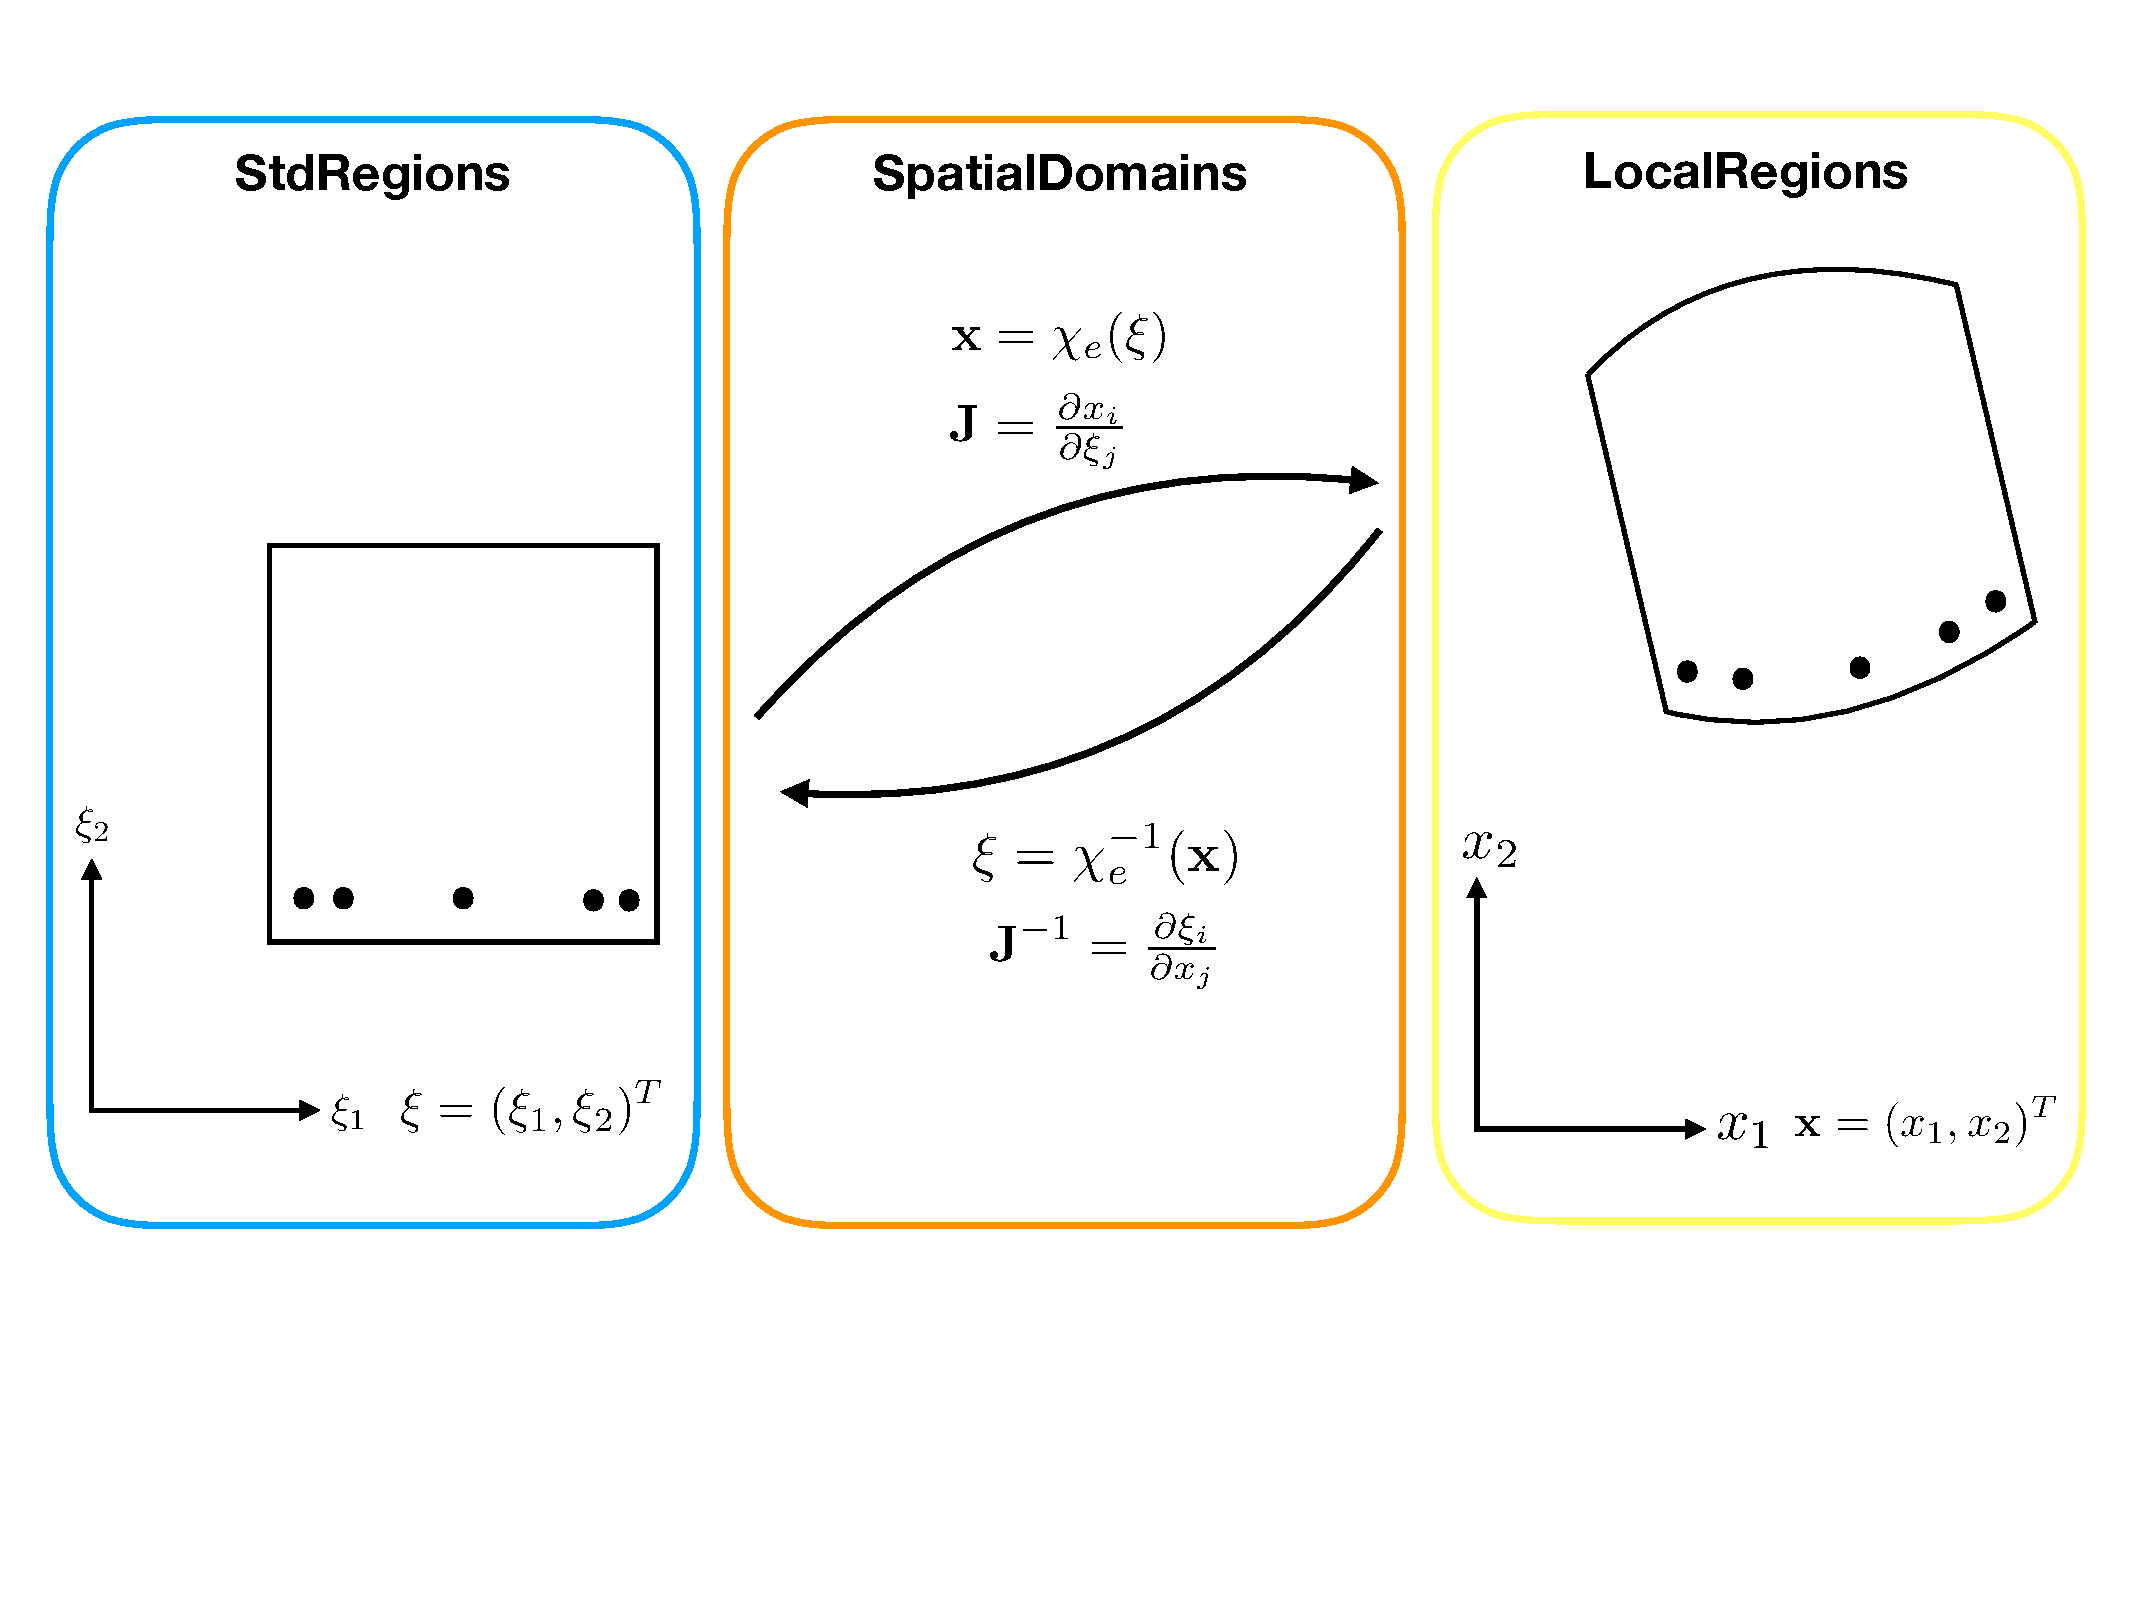
\includegraphics[width=4in]{img/stdtolocal.pdf}
\caption{Diagram showing the LocalRegion (yellow) {\em is-a} StdRegion (blue) which {\em has-a} SpatialDomain (orange) in terms of coordinate systems and mapping functions. This diagram highlights how points (positions in space) are mapped between different (geometric) regions.}
\label{intro:stdtolocal}
\end{figure}

Since $\Psi$ lives on $E_S = [-1,1] \times [-1,1]$ (i.e. $\Psi:E_S\rightarrow\mathbb{R}$) and is for this example polynomial, we can integrate it exactly (to machine precision) using Gaussian integration, and we can differentiate it by writing it in a Lagrange basis and forming a differential operator matrix to act on values of the function evaluated at points.   If the function were not polynomial but instead only a smooth function, we could approximate it with quadrature and decide an appropriate basis by which to 
approximate its derivatives.  All the routines needed for differentiating and integrating polynomials over various standard regions are contained within the StdRegions 
directory (and will be discussed in Chapter \ref{chap:stdregions}).   A local region expansion, such as a basis defined on a quadrilateral element, QuadExp, is a linear combination of basis functions over its corresponding standard region as mapped by
information contained within its spatial domain mapping.  Local region class definitions are in the LocalRegions directory (and will be discussed in Chapter \ref{chap:localregions}).  Using the inheritance language of C++, we would say that a local region {\em is-a} standard region and
{\em has-a} spatial domain object.  The SpatialDomains directory contains information that expresses the mapping function $\chi(\cdot)$ from the standard region
to a local region.  SpatialDomains is explored in Chapter \ref{chap:spatialdomains}.  In the case of our quad example, the SpatialDomain object held by a QuadExp would connect the local region to its StdRegion parent,
and correspondingly would allow integration and differentiation in world space (i.e., the natural coordinates in which the local expansion lives).  If $E$ denotes our
geometric region in world space and if $F:E\rightarrow\mathbb{R}$ is built upon polynomials over its standard region, then we obtain $F(x_1,x_2) = \Psi(\chi^{-1}(x_1,x_2))$.  Note that even though $\Psi$ is polynomial and $\chi$ is polynomial, the composition using the inverse of $\chi$ is not guaranteed to be polynomial: it is only
guaranteed to be a smooth function. 

Putting this in the context of MultiRegions, we arrive at Figure \ref{intro:structure1}.  The MultiRegions directory (which will be discussed in Chapter \ref{chap:multiregions}) contains various data structures that combine
local regions.  One can think of a multi-region as being a set of local region objects in which some collection of geometric and/or function properties are enforced.
Conceptually, one can have a set of local region objects that have no relationship to each other in space.   This is a set in the mathematical sense, but not really
meaningful to us for solving approximation properties.  Most often we want to think of sets of local regions as being collections of elements that are geometrically
contiguous -- that is, given any two elements in the set, we expect that there exists a path that allows us to trace from one element to the next.   Assuming
a geometrically continuous collection of elements, we can now ask if the functions built over those elements form a piece-wise discontinuous approximation
of a function over our multiregion or a piece-wise continuous $C^0$ approximation of a function over our multiregion.

\begin{figure}[htb]
\centering
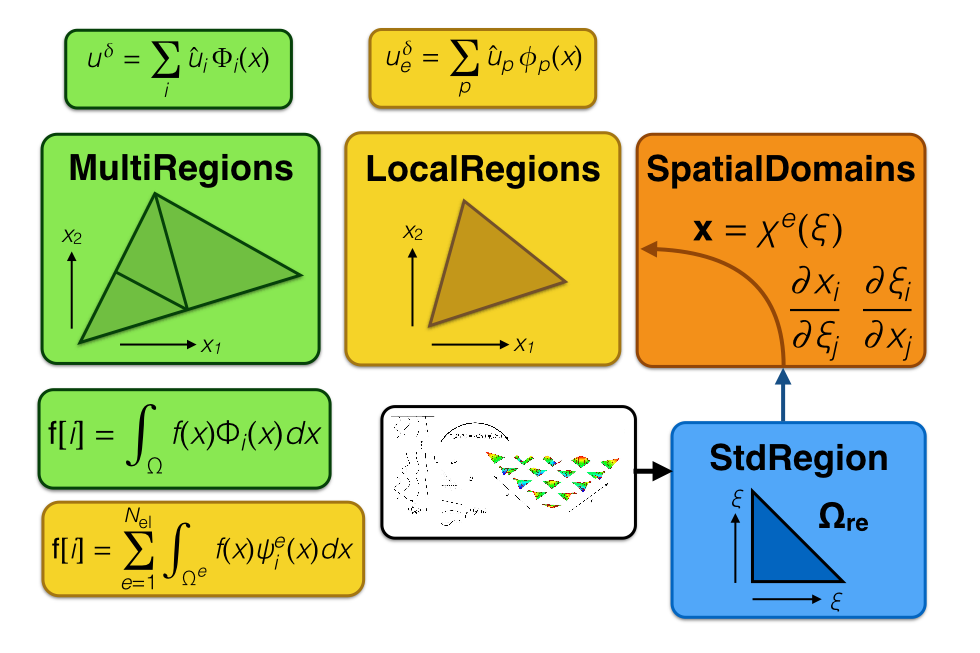
\includegraphics[width=4in]{img/structure1.png}
\caption{Diagram showing how a MultiRegion (green) contains a collection of LocalRegions (yellow), where a LocalRegion {\em is-a} StdRegion (blue) which {\em has-a} SpatialDomain (orange) in terms of coordinate systems and mapping functions.  This diagram highlights the expansions of the solution formed over each geometric domain.}
\label{intro:structure1}
\end{figure}


%%%%%%%%%%%%%%%%%%%%%%%%%%%%%%
\subsubsection{Top-Down Perspective}

The top-down perspective on the library is best understood from Figure \ref{intro:structure2}.  From this perspective, we are interested in understanding 
{\nek} from the solvers various people have contributed.  

\begin{figure}[htb]
\centering
\includegraphics[width=4in]{img/structure2.png}
\caption{Diagram showing the top-down perspective on library components.  Various solvers (along the top) can capitalize on generic SolverUtils and are built upon
the core {\nek} libraries consisting of MultiRegions (green), Collections (red), LocalRegions (yellow), SpatialDomains (orange) and StdRegions (blue).  The most 
generic mathematical and computer science features are contained within LibUtilities, which in part draws from various community resources such as Boost, Metis, etc.}
\label{intro:structure2}
\end{figure}


\section{Assumed Proficiencies}

This developer's guide is designed for the experienced \shp{} user who wishes to go beyond
using various \nek{} solvers and possibly to add new features or capabilities at the library,
solver or utilities levels.  Since the focus of this document is \nek{}, we cannot 
recapitulate all relevant mathematical or computer science concepts upon which our
framework is built.  In this section we provide a listing of areas and/or topics of 
assumed knowledge, and we provide a non-exhaustive list of references to help
the reader see the general areas of additional reading they may need to benefit fully
from this manual.

We assume the reader has a familiarity and comfort-level with the following areas:

\begin{enumerate}
\item Finite Element Methods (FEM) ~\cite{Hughes87,Schwab,BaSzKa81} and more generally the mathematical ideas 
surrounding continuous Galerkin (cG) methods.  This includes basic calculus of variation concepts, basic
partial differential equation knowledge, and general forms of discretization and approximation.

\item Polynomial Methods~\cite{CanutoHQZ87,Funaro92,HGG}, and in particular concepts surrounding polynomial
spaces, basis functions and numerical differentiation and quadrature.

\item Spectral Element Methods (SEM)~\cite{DevilleFM02,KaSh05}.

\item Discontinuous Galerkin Methods \cite{CockburnKS,HesthavenW08}.

\item Scientific Computing~\cite{Heath,KarniadakisK03}.  We assume a graduate-level proficiency in basic
computational techniques such as dealing with numerical precision (accuracy and conditioning), root-finding algorithms,
differentiation and integration, and basic optimization.

\item Linear Algebra \cite{TrefethenB97,Demmel97}.  We assume a strong knowledge of linear algebra and a reasonable 
comfort level with the various numerical algorithms used for the solution of symmetric and non-symmetric linear systems.
\end{enumerate}

\section{Other Software Implementations and Frameworks}

In the last ten years a collection of software frameworks has been put forward to try to bridge the gap between the 
mathematics of high-order methods and their implementation. 
A number of software packages already exist for fluid dynamics which implement
high-order finite element methods, although these packages are typically targeted at a specific
domain or provide limited high-order capabilities as an extension.
A major challenge many practitioners have with
spectral/{\em hp\/} elements and high-order methods, in general, is the complexity (in terms of algorithmic design) they
encounter. In this section, we give an incomplete but
representative summary of several of these attempts to overcome this challenge.

The \emph{Nektar flow solver} is the predecessor to \nek{} and
implements the \shp{} element method for solving the incompressible
and compressible Navier-Stokes equations in both 2D and 3D. While it is widely
used and the implementation is computationally efficient on small parallel problems,
achieving scaling on large HPC clusters is challenging. Semtex \cite{BlSh04}
implements the 2D spectral element method coupled with a Fourier expansion in
the third direction. The implementation is highly efficient, but can only be
parallelised through Fourier-mode decomposition.
Nek5000 \cite{Nek5000} is a 3D spectral element code, based on hexahedral
elements, which has been used for massively parallel simulations up to 300,000
cores. The Non-hydrostatic Unified Model of the Atmosphere (NUMA) \cite{GiraldoKC13} is a spectral element framework that employs continuous 
and discontinuous Galerkin
strategies for solving a particular problem of interest, but in a way on which others could adopt and build.  
Hermes \cite{VeSoZi07} implements hp-FEM for two-dimensional problems and
has been used in a number of application areas. Limited high-order finite
element capabilities are also included in a number of general purpose PDE
frameworks including the DUNE project \cite{DeKlNoOh11} and deal.II
\cite{BaHaKa07}.
% %
FEniCS \cite{FEniCS} is a collaborative project for the development of scientific computing tools, with a particular focus 
on the automated solution of differential equations by finite element methods (FEM).  Through the use of concepts such as meta-programming,
FEniCS tries to keep the solving of PDEs with FEM, from the application programmers' perspective, as close to the mathematical expressions
as possible without sacrificing computational efficiency.
%%
A number of codes also implement high-order finite element methods on
GPGPUs including nudg++, which
implments a nodal discontinuous Galerkin scheme \cite{HeWa07}, and PyFR
\cite{WiFaVi14}, which supports a range of flux reconstruction techniques.

\section{How to Use This Document}

In the next chapter, we will introduce the reader to various computer science tools and ideas upon which we rely heavily in our development and deployment of {\nek}.  The remainder of this developer's guide is then partitioned into three parts.

In Part \ref{part:library}, we provide an overview of the various data structures and algorithms that live within the {\em library} subdirectory.  We think of the library as containing all the basic building blocks of the {\nek} code, as discussed above.  In this part of the developer's guide, we have dedicated a chapter to each subdirectory within the library.  Each chapter contains three main sections.  The first section of a chapter provides an overview of the mathematical concepts and terminology used within the chapter.  This is not meant to be a detailed tutorial, but rather a reminder of basic concepts.  The second section of a chapter provides a detailed description of the data structures introduced in that part of the library.  The third section of a chapter is dedicated to explaining the algorithmic aspects of the library.  Instead of going function by function or method by method, we have decided to structure this section in the style of ``frequently asked questions" (FAQ).  Based upon our long experience with students, postdocs and collaborators, we have distilled down a collection of questions that we will use (from the pedagogical perspective) to allow us to drill down into key algorithmic aspects of the library.

In Part \ref{part:solvers}, we provide an overview of the many solvers implemented on top of the {\nek} library.  Each chapter is dedicated to a different solver, and correspondingly may take on a slightly different style of presentation to match the depth of mathematical, computer science and engineering knowledge to understand the basic data structures and algorithms represented there.

In Part \ref{part:utilities}, we provide an overview of many of the utilities often used in our simulation pipeline -- from things that aid the user in the preprocessing steps such as setting up parameter files and meshing to the postprocessing step of field conversion for visualization.

How you engage with this material is based upon your goals.  If your goal is to:

\begin{itemize}
\item Introduce a new solver, then you would want to jump to Part \ref{part:solvers} and see how other solvers have been built.  Then, depending on what library functions are needed, you may need to step back into the library parts of this manual to understand how to use some of our basic library functionality.
\end{itemize} 








%

\chapter{Preliminaries}


%%%%%%%%%%%%%%%%%%%%%%%%%%%%%%%%%%%%%%%%%%%%%%%%%%
\section{Summary of Development Tools and Best Practices}

%%%%%%%%%%%%%%%%%%%%%%%%%%%%%%%%%%%%%%%%%%%%%%%%%%

\subsection{General Resources}

\subsubsection{Mailing List}

Please make sure that you sign up to the {\nek} mailing list. This can be done at the following URL:

\url{https://mailman.ic.ac.uk/mailman/listinfo/nektar-users}

While the name suggests it is for \textit{users} of Nektar++, this list is also used to ask questions about {\nek} development.

\subsubsection{Blog}

The {\nek} blog (\url{https://www.nektar.info/cat/community})
provides a broad range of posts on topics such as compiling the code
on specific machines, to discussions of {\nek} in specific
application areas, to recently published papers which have made use of
the code.

Contributing to this resource is a valuable way to support the project, as well as promoting your own work.

\subsubsection{Annual Workshop}

In 2015, we held the first {\nek} workshop, which was a great
success and followed by a similar event in 2016. It is now an annual
event and allows first-hand access to the core {\nek} development
team as well as a range of other {\nek} users.

%%%%%%%%%%%%%%%%%%%%%%%%%%%%%%%%%%%%%%%%%%%%%%%%%%

\subsection{Version Control (git)}
\lstset{style=BashInputStyle}

The {\nek} code is managed in a distributed version control system called {\GIT}. To obtain the code directly from the repository and add new content to the repository requires the \texttt{git} command-line tool (or a suitable GUI equivalent). This is available for Linux, Mac OSX and Windows.

If you plan to work with the {\nek} community, you will
need to have a reasonable understanding of the {\GIT}
software.  While it is beyond the scope of this document to discuss
how to use {\GIT}, it is important for someone new to {\GIT} to spend
time understanding how the tool works.  For this purpose, we highly
recommend familiarizing yourself with it using any of the many online
resources (such as \texttt{https://git-scm.com}).

\subsubsection{Anonymous Access}

{\nek} may be cloned anonymously using the following command:

\code{git clone http://gitlab.nektar.info/clone/nektar/nektar.git nektar++}

Your local copy of the code can be updated to include the latest changes in the repository using the command:

\code{git pull}

The \emph{Anonymous Access} approach will provide you with a complete copy of the code, but you will be unable to push changes or new developments back to the repository. For this, you should use \emph{Collaborative Access}.


\subsubsection{Collaborative Access}

Once you are familiar with {\GIT}, have introduced yourself to the
development community (see the mailing list information above), and
are ready to become a contributing developer, you will need to register
an account on the {\nek} Gitlab website:

\url{https://gitlab.nektar.info}.

To use use authenticated access, using your new account, you must first upload the \textbf{public} part of your SSH key to your Gitlab profile. Generating and managing SSH keys is beyond the scope of this document. However, on Linux and OSX, one generally finds these keys in the \lstinline{\$HOME/.ssh} directory.

To upload the key, visit: \url{https://gitlab.nektar.info/profile}, select \emph{SSH keys} from the menu on the left and follow the instructions.

Registering for an account and uploading your SSH key need only be done once.

To clone {\nek}, use the {\GIT} command:

\code{git clone git@gitlab.nektar.info:nektar/nektar.git nektar++}

Note the different URL to use authenticated access, in comparison to the anonymous access.


\subsubsection{Managing and Contributing code}
Code contribution then follows three basic steps:
\begin{enumerate}
    \item Create an \emph{issue} to describe the code updates you are making;
    \item Branch the {\nek} master branch and make your changes on that branch; and 
    \item Submit a merge request on the {\nek} Gitlab website that your updates are ready to be merged into the master branch.
\end{enumerate}

More details regarding the concepts mentioned above is found below. The information is also available in the \texttt{CONTRIBUTING.md} file in the root directory of the code, or online at:
\url{https://gitlab.nektar.info/nektar/nektar/blob/master/CONTRIBUTING.md}

\begin{itemize}
  \item Issues - The initial step for those who wish to add code to the
  master repository is to create an \emph{issue} ticket that describes the
  defect, bug, proposed additions, changes, updates, etc.  This is done on the Gitlab website at:
  
  \url{https://gitlab.nektar.info/nektar/nektar/issues}

  Please ensure you provide sufficient detail when creating the issue to cover
  all of the following (as required): Describe what is being
  requested, why it is important / necessary, an initial list of files
  that may be effected, any potential problems the change/addition may
  cause, and any other information that will help the development team
  understand the request and alert others to your work to avoid duplication of effort.
  
  \item Branches - The second step is to create a {\GIT} branch in which to do
  the actual code development. In your local copy of the {\nek} repository, run the command:
  \begin{lstlisting}  
  git branch <branch-name>
  \end{lstlisting}
  replacing \lstinline{<branch-name>} with a suitable name for your branch. The naming convention used for branches reflects the nature of the change and is composed of a prefix and descriptor, separated by a forward slash. Prefixes are one of:
  \begin{itemize}
      \item \texttt{feature}: used for developments which constitute a new capability in the code;
      \item \texttt{fix}: used for changes to fix a bug in the code;
      \item \texttt{tidy}: used for changes which improve the quality or readability of the code but do not change its function;
      \item \texttt{ticket}: can be used to reference changes which address a specific issue.
  \end{itemize}
  Please choose concise descriptors in all-lowercase, using hyphens to separate words. An example \lstinline{<branch-name>} might therefore be: \lstinline{feature/low-energy-preconditioner}
  
  Now make your new branch active by running the command:
  \begin{lstlisting}
  git checkout <branch-name>
  \end{lstlisting}
  Confirm you are on the correct branch by running:
  \begin{lstlisting}
  git status
  \end{lstlisting}
  which should print something similar to
  \begin{lstlisting}
  On branch <branch-name>
  \end{lstlisting}

  At this point you are all set to make the required modifications to the 
  code in your branch.  As you modify your branch, you can use {\GIT} to
  save and track your changes.

  The following examples show how you can add a file to the list of local
  files that are being tracked, display differences between the current
  file and the original file, and commit the file.  
  \begin{lstlisting}
  git add library/LibUtilities/BasicUtils/my_new_file.cpp
  git diff --cached
  \end{lstlisting}

  Note \lstinline{--cached} is necessary because \lstinline{my\_new\_file.cpp} was staged using
  the \lstinline{git add} command above.  Note, before you add (stage) the
  file, you can just use \lstinline{git diff}.
  
  To actually create the commit from the staged files, run:
  \begin{lstlisting}
  git commit -m "Added X, Y, Z..."
  \end{lstlisting}
  This commits the file to your local repository. The first line of the log message should be a concise summary of the changes. You can use subsequent lines to provide more details if needed. Use \lstinline{git log} to see the list of previous commits and their messages.
  
  These changes are still local to your computer. To push them up to the main {\nek} repository, use the command
  \begin{lstlisting}
  git push origin
  \end{lstlisting}
\end{itemize}

%%%%%%%%%%%%%%%%%%%%%%%%%%%%%%%%%%%%%%%%%%%%%%%%%%
\subsection{Building (CMake)}

{\nek} uses the \emph{CMake} tool to manage the build process for
the three supported operating systems: Linux, Windows, and OSX.  For
detailed instructions on how to use \emph{CMake} to build {\nek},
including a list of required software dependencies and \emph{CMake}
option flags, please refer to the {\nek} User Guide section 1.3.

\subsection{Testing (CTest)}
Before you are ready to have your code merged into the {\nek}
trunk, you should make sure that it passes the built-in test suite -
in addition to any new tests that you have added for your
updates. To run the test suite, on the command line type:
\begin{lstlisting}  
ctest [-j#]
\end{lstlisting}
  
The \lstinline{-j#} optional argument will run \lstinline{#} tests in parallel
taking advantage of multiple cores on your machine.  It is highly
recommended that your use all available cores to minimize the amount
of time spent waiting for the tests to complete. There are currently
several hundred built-in unit tests for {\nek}.

For more information on testing, see ``Software Testing Approaches'' below.

\subsection{Merge Requests (Gitlab)}
The final step in contributing your code to the
Nektar master repository is to submit a merge request to the
development team using the {\nek} gitlab website:
  
\url{https://gitlab.nektar.info/nektar/nektar/merge\_requests}
  
Submitting a merge request will automatically trigger the continuous integration (CI) system, which will build and test your code on a range of platforms. You can monitor the progress of these tests from the merge request page. Selecting individual workers will take you to the buildbot website from which you can examine any failures which have occurred.
  



%%%%%%%%%%%%%%%%%%%%%%%%%%%%%%%%%%%%%%%%%%%%%%%%%%
\section{Core Nektar++ Programming Concepts}
\lstset{style=C++Style}

This section highlights some of the programming features that are used
extensively within {\nek}. While much of the code consists of
standard C++ practices, in some of the core infrastructure there are
several practices that may be only familiar to programmers who have
developed code using more advanced C++ features.  Below we give a
short summary of these entities in order to provide a starting point
when working with these features. We begin with more well known
features and end with some advanced techniques.  Note, it is not the
purpose of the following sections to cover in detail each of these
important concepts, but instead to give a brief overview of them such that the developer may look to other, more in-depth, sources if
they require further guidance.

\subsection{Namespaces}
Many C++ software projects place their code in a namespace so as to avoid conflicts with other code when included in larger applications.  It is important to note that {\nek} uses a hierarchy of namespaces for most of the defined data structures.  The top level namespace is always ``Nektar'', with the second level usually corresponding to the name of the library to which the code belongs. For example:
\begin{lstlisting}
namespace Nektar
{
namespace StdRegions
{
    ...
}
}
\end{lstlisting}

With this in mind, when you see something like \lstinline{Nektar::SpatialDomains::...}, you can usually assume that the second item (in this case \lstinline{SpatialDomains}) is a namespace, and not a class.

\textbf{Note:} To make better use of the 80 character width, generally enforced across the {\nek} source code, we choose not to indent the contents of \lstinline|namespace| blocks.


\subsection{C++ Standard Template Library (STL) }
{\nek} uses of the C++ STL extensively.  This consists of common data structures and algorithms, such as map and vector, as well as many of the extensions once found in the Boost library that have become part of the C++ standard and are now used directly.

One of the most important of these features is
the use of Shared Pointers (\lstinline|std::shared_ptr|).  Most developers are
somewhat familiar with ``smart pointers'' (pointers used to track
memory allocation and to automatically deallocate the memory when it
is no longer being used) for data blocks that are shared by multiple
objects. These smart pointers are used extensively in {\nek} and
one should be familiar with the \lstinline|dynamic_pointer_cast| function
and the concept of the \lstinline|weak_ptr|.  Dynamic casting allows for safely
converting one type of variable into its base type (or vice
versa). For example:
\begin{lstlisting}
std::shared_ptr<FilterCheckpoint> sptr =
        std::dynamic_pointer_cast<FilterCheckpoint>( m_filters[k] );
if( sptr != nullptr ) 
{ 
   // Cast succeeded!
}
\end{lstlisting}

The advantage of using the dynamic cast, in comparison to the C style
cast, is that you can check the return value at run time to verify
that the casting was valid.  A \lstinline|weak_ptr| is a pointer to shared
data with the explicit contract that the weak pointer does not own
the data (and thus will not be responsible for deallocating it).
Weak pointers are used mostly for short-term access to shared data.

Another modern code utility used by {\nek} to support shared
pointers can be seen in {\nek} classes which inherit from
\lstinline|std::enable_shared_from_this|. This allows a class member function to return a shared pointer to itself. Specifically, it makes available the function \lstinline|shared_from_this()| which returns a shard pointer to the object in the given context.

While C++ shared pointers are a powerful resource, there are a
number of intricacies that must be understood and followed when
creating classes and using objects that will be managed by them.
For those not familiar with the C++11 (or previously Boost)
implementation, it is highly recommended that you study them in more
detail then presented here.
  
\subsection{typedefs}
Like most other large codes, {\nek} uses
\lstinline{typedefs} to create short names for new variable types.  You will
see examples of this throughout the code and taking a few minutes to
look at the definitions will help make it easier to follow the code.
In the following example, we create (and explicitly name) the type
\lstinline{ExpansionSharedPtr} to make the code that uses this type easier
to follow. This is particularly true of nested STL data structures where repeated template declarations would make the code harder to follow. A couple of examples are shown below:
\begin{lstlisting}
typedef std::shared_ptr<Expansion> ExpansionSharedPtr;
typedef std::shared_ptr<std::vector<std::pair<GeometrySharedPtr, int>>>
GeometryLinkSharedPtr;
\end{lstlisting}
If you are not familiar with the use of typedefs, you should take
time to read about them (there are many short summaries
available on the web).

\subsection{Forward Declarations}
There are two ways that an existing class
type can be specified when declaring a new class in a header file.  The
existing class can either be declared in name only, or declared in its entirety, before being used. In the latter case, one typically includes the header file declaring the full class. If the new class declaration only references the existing class in the form of a pointer or reference then the entire class declaration is not needed and the compiler only needs an assurance that the class exists. For this case, we can use a \emph{forward declaration} which tells the compiler the name of the existing class. 
However, if functions of the existing class are called (within the new header file) or the class is used by value, then the full declaration is needed.

Forward declaring a class is achieved as shown in the following example:
\begin{lstlisting}
class LinearSystem;
\end{lstlisting}
This statement tells the compiler the class \lstinline{LinearSystem} exists and, as long as we only make reference to it as a pointer (\lstinline{LinearSystem* l}) or by reference (\lstinline{const LinearSystem & l}), then the compiler does not require any further information.

An advantage to using forward declarations where possible is that the header file does not need to \lstinline{#include} the entire existing class and any header files referenced within.  This allows for a
cleaner header files and faster compilation as the compiler can process (often significantly) fewer lines of code.

\textbf{Note}: The full class declaration is most likely needed in the new class implementation file (.cpp) as reference to the existing class's members will presumably be made.
  
\subsection{Templated Classes and Specialization}
Most C++ developers are
familiar with basic class templating.  However, many have not needed
to use explicit template specialization.  This is the process of
implementing customised behaviour for one or more of the specific instances of a template when
the compiler will not be able to instantiate a generic version for
the class, or when different code is needed based on different
versions of the class.  For example:
\begin{lstlisting}
  template<typename Dim, typename DataType> 
  class Array;
  
  template<typename DataType>
  class Array<OneD, const DataType> {
    // Explicit coding of class methods and variables specific to
    // this version of Array are found here.
  };
\end{lstlisting}

In the above example, on the first line the generic templated
\lstinline{Array} class is declared. There are two template parameters: the dimension and the element type. The second line shows an explicit
template specialisation of the \lstinline{Array} class for a one-dimensional (version of) \lstinline{Array}.  When explicitly specialising a class, the programmer
will write code that is specific to the datatype used in specifying
the class.  This includes explicitly writing code for one, some, or
all of the methods of the class.

It is important to understand template specialization when dealing
with the {\nek} core libraries so that the developer can
determine which (specialized version of the) class is being used,
and to know that when updating classes with varied specializations,
that it may be required to update code in several places (ie, for
each of the specializations).

\subsection{Multiple Inheritance and the \lstinline{virtual} Keyword}
When diving into many {\nek} classes, you will see the use of multiple
inheritance (where a class inherits from more than one parent
class).  When the parent class does not inherit from other classes,
then the inheritance is straightforward and should not cause any
confusion.  However, when a class has grandparents, many times that
grandparent class is the same class but is inherited through multiple
parents.  To account for this, class inheritance should use the
\lstinline{virtual} keyword.  This specifies that if a class has multiple
grandparents (that happen to be the same class), that only one copy of
the grandparent class members should actually be instantiated. For example:
\begin{lstlisting}
class Expansion2D : virtual public Expansion,
                    virtual public StdRegions::StdExpansion2D
{...}
\end{lstlisting}


\subsection{Virtual Functions and Inheritance}
Within {\nek}, classes
that inherit from a parent class and override one of the parent
class methods, use the concept of virtual functions. The function is prefixed with a \lstinline{v_}, such as \lstinline{v_Function()}, as a naming convention.  This is a visual reminder that the function overrides a parent class function. For example:
\begin{lstlisting}
NekDouble TriExp::v_Integral(const Array<OneD, const NekDouble> &inarray)}
\end{lstlisting}

\subsection{Const keyword}
While the \lstinline{const} keyword is known to most C++
developers, it is used (as it should be) liberally in {\nek} for functions,
function parameters, returning pointers to class data, and variable
constants within functions.  It is easy to neglect using \emph{const}
to mark all cases where a variable should be considered constant.
However, its use can substantially reduce accidental errors and
allow for accelerated debugging. The \lstinline{const} qualifier should be used wherever a variable does not change including 1) parameters passed to
functions, 2) variables in functions (or classes) that do not change
value during their lifetime, 3) on the return type of functions that return pointers to data that should not be changed, and 4) on methods that do not
change data within the class. The compiler will then produce an error if we (accidentally) attempt to make a change which violates a \lstinline{const}.

\subsection{Function pointers and bind}
Function pointers
  (\lstinline{std::function}) are similar to pointers to data, except that
  they point to functions - and thus allow a function to be invoked
  indirectly (in other words, without explicitly writing the function
  call (name) directly in code).  This technique is used by {\nek}
  in a number of places, with \lstinline{NekManager} being a prime example.
  The \lstinline{NekManager} class is used to create objects of a specific
  type during the execution of the program.  When a \lstinline{NekManager} is
  created (constructed), it is provided with a pointer to a function
  that will (later) be called to generate the objects to be managed when required.  While
  the \emph{creation} function that is provided to the \lstinline{NekManager}
  takes a number of parameters, in many cases some of the values to
  those parameters will be fixed.  To handle this situation, {\nek}
  uses the \lstinline{std::bind( f )} function, which creates a new function
  based on supplied original function \lstinline{f}, but specifies that one
  or more parameters of \lstinline{f} are fixed at the time that \lstinline{f} is created and only those bound parameter values will be used when
  \lstinline{f} is later invoked.  


\subsection{Memory Pools and NekArray}
An Array is a thin wrapper around native arrays. Arrays provide all the
functionality of native arrays, with the additional benefits of automatic use of
the Nektar++ memory pool, automatic memory allocation and deallocation, bounds
checking in debug mode, and easier to use multi-dimensional arrays.

Arrays are templated to allow compile-time customization of its dimensionality
and data type.

Parameters:
\begin{itemize}
    \item \lstinline{Dim} Must be a type with a static unsigned integer called
    \lstinline{Value} that specifies the array's dimensionality. For example
    \begin{lstlisting}
    struct TenD {
        static unsigned int Value = 10;
    };
    \end{lstlisting}
    \item \lstinline{DataType} The type of data to store in the array.
\end{itemize}

It is often useful to create a class member Array that is shared with users of
the object without letting the users modify the array. To allow this behavior,
\lstinline{Array<Dim, DataType>} inherits from 
\lstinline{Array<Dim, const DataType>}. The following
example shows what is possible using this approach:
\begin{lstlisting}
class Sample {
public:
    Array<OneD, const double>& getData() const { return m_data; }
    void getData(Array<OneD, const double>& out) const { out = m_data; }

private:
    Array<OneD, double> m_data;
};
\end{lstlisting}
In this example, each instance of Sample contains an array. The getData
method gives the user access to the array values, but does not allow
modification of those values.



%%%%%%%%%%%%%%%%%%%%%%%%%%%%%%%%%%%%%%%%%%%%%%%%%%
\section{Design Patterns}
\subsection{Template pattern}
\label{s:template-pattern}
The template pattern is used frequently within {\nek} to provide a common interface to a range of related classes. The base class declares common functionality or algorithms, in the form of public functions, deferring to protected virtual functions where a specific implementation is required for each derived class. This ensures code external to the class hierarchy sees a common interface.

In the top level parent class you will find the interface functions, such as
\lstinline{Function()}, declared as public members. In some cases, these may implement a generic algorithm common to all classes. In the limit that the function is entirely dependent on the derived class, it may call through to a virtual counterpart, usually named \lstinline{v_Function()}. These functions are usually protected to allow them to be called directly by other classes in the inheritance hierarchy, without exposing them to external classes.

As an example of this, let us consider a triangle
element (\lstinline{TriExp}).  The \lstinline{TriExp} class (eventually) inherits from the \lstinline{StdExpansion} class.  The \lstinline{StdExpansion} defines the \lstinline{Integral()} function which is used to provide integration over an element.  However, in this case, the implementation is shape-specific. Therefore \lstinline{StdExpansion::Integral()} calls the (in this case) \lstinline{TriExp::v_Integral()} function.  We should also note that while \lstinline{TriExp::v_Integral()} does setup work, it then makes use of its parent's \lstinline{StdExpansion2D::v_Integral()} function to calculate the final value. This is only possible if the \lstinline{v_Integral()} function was declared as protected.

\subsection{Abstract Factory Pattern}

{\nek} makes extensive use of the \emph{Factory Pattern}.
Factories are used to create (allocate) instances of classes using class-specific creator functions. More
specifically, a factory will create a new object of some
sub-class type but return a base class pointer to the new
object. In general, there are two ways that a factory knows what
specific type of object to generate: 1) The Factory's build
function (\lstinline{CreateInstance()}) is
passed a key that details what to build; or 2) The factory may
have some intrinsic knowledge detailing what objects to create. The first case is almost exclusively used throughout {\nek}.
The factory pattern provides the following benefits:
\begin{itemize}
\item Encourages modularisation of code such that conceptually related
algorithms are grouped together;
\item Structuring of code such that different implementations of the same
concept are encapsulated and share a common interface;
\item Users of a factory-instantiated modules need only be concerned with the
 interface and not the details of underlying implementations;
\item Simplifies debugging since code relating to a specific implementation
 resides in a single class;
\item The code is naturally decoupled to reduce header-file dependencies and
 improves compile times;
\item Enables implementations (e.g. relating to third-party libraries) to be
 disabled through the build process (CMake) by not compiling a specific 
 implementation, rather than scattering preprocessing statements throughout the
 code.
\end{itemize}


\subsubsection{Implementing the factory pattern}
The \lstinline{NekFactory} class implements the factory pattern in Nektar++.
There are two distinct aspects to creating a factory-instantiated collection of
classes: defining the public interface, and; registering specific
implementations. Both of these tasks involve adding mostly standard boilerplate code.

It is assumed that we are writing a code which implements a particular \emph{concept} or
\emph{capability} within the code, for which there are (potentially) multiple implementations. The
reasons for multiple implementations may be low level, such as alternative
algorithms for solving a linear system, or high level, such as selecting from a
range of PDEs to solve. The \lstinline{NekFactory} can be used in both cases and applied in exactly the same way.

\subsubsection{Creating a concept (base class)}
A base class must be defined which prescribes an implementation-independent
interface. In Nektar++, the template method pattern (see Section~\ref{s:template-pattern} above) is used, requiring public
interface functions to be defined which call through to protected virtual implementation methods. This is because the factory returns the newly created object via a base-class pointer and the objects will almost always be used via this base class pointer. Without a public interface in the base class, much of the benefits and generalisation of code offered by the factory pattern would be lost.
The virtual functions will be overridden in the specific implementation classes.
In the base class these virtual methods should normally be defined as pure virtual, since there is typically no implementation and we will never be explicitly instantiating this base class.

As an example we will create a factory for instantiating different
implementations of some concept \inlsh{MyConcept}, defined in
\inlsh{MyConcept.h} and \inlsh{MyConcept.cpp}.

First in \inlsh{MyConcept.h}, we need to include the NekFactory header
\begin{lstlisting}
#include <LibUtilities/BasicUtils/NekFactory.hpp>
\end{lstlisting}

The following code should then be included just before the base class
declaration (within the same namespace as the class):
\begin{lstlisting}
class MyConcept

// Datatype for the MyConcept factory
typedef LibUtilities::NekFactory< std::string, MyConcept, 
            ParamType1,
            ParamType2 > MyConceptFactory;
MyConceptFactory& GetMyConceptFactory();
\end{lstlisting}

The template parameters to the \lstinline{NekFactory} define the datatype of the key used to retrieve a
particular implementation (usually a string, enum or custom class such as
\lstinline{MyConceptKey}), the base class datatype (in our case \lstinline{MyConcept} and a list
of zero or more parameters which are taken by the constructors of all
implementations of the type \lstinline{MyConcept} (in our case we have two). Note
that all implementations must take the same parameter list in their constructors. Since we have not yet declared the base class type \lstinline{MyConcept}, we have forward-declared it above the \lstinline{NekFactory} type definition.

The normal definition of our base class then follows:
\begin{lstlisting}
class MyConcept 
{
    public:
        MyConcept(ParamType1 p1, ParamType2 p2);
        ...
};
\end{lstlisting}

We must also define a shared pointer for our base class, which should be declared outside the base class declaration.
\begin{lstlisting}
typedef boost::shared_ptr<MyConcept> MyConceptShPtr;
\end{lstlisting}


\subsubsection{Creating a specific implementation (derived class)}
A new class, derived from the base class above, is defined for each specific implementations of a concept. It is these
specific implementations which are instantiated by the factory.

In our example we will have an implementations called \lstinline{MyConceptImpl1}
defined in \inlsh{MyConceptImpl1.h} and \inlsh{MyConceptImpl1.cpp}. In the
header file we include the base class header file
\begin{lstlisting}
#include <MyConcept.h>
\end{lstlisting}

We then define the derived class as one would normally:
\begin{lstlisting}
class MyConceptImpl1 : public MyConcept
{
...
};
\end{lstlisting}

In order for the factory to work, it must know two things:
\begin{itemize}
\item that \lstinline{MyConceptImpl1} exists; and
\item how to create an instance of it.
\end{itemize}

To allow the factory to create instances of our class we define a \emph{creator} function in our class, which may have arbitrary name, but is usually called \lstinline{create} out of convention:
\begin{lstlisting}
/// Creates an instance of this class
static MyConceptSharedPtr create(
            ParamType1 p1,
            ParamType2 p2)
{
    return MemoryManager<MyConceptImpl1>::AllocateSharedPtr(p1, p2);
}
\end{lstlisting}
The example above the \lstinline{create} function simply creates an instance of \inlsh{MyConceptImpl1} using the {\nek} memory manager and the
supplied parameters. It must be a \lstinline{static} function because we are not operating on any existing instance and it should return a shared pointer to a base class object (rather than a \lstinline{MyConceptImpl1} shared pointer), since the point of the factory is that the calling code does not know about specific implementations. An advantage of having each class providing a creator function is that it allows for \emph{two-stage initialisation} -- for example, initialising base-class variables based on the derived type.

The final task is to register each of our implementations with the factory. This is done 
using the \lstinline{RegisterCreatorFunction} member function of the \lstinline{NekFactory}.
However, we wish this to happen as early on as possible (so we can use the 
factory straight away) and without needing to explicitly call the function for 
every implementation at the beginning of our program (since this would again 
defeat the point of a factory)! One solution is to use the function to 
initialise a static variable: it will force the function to be executed prior to the start of the \lstinline{main()} routine, and can be located within the class it is registering, satisfying our code decoupling requirements.

In \inlsh{MyConceptImpl1.h} we define a static class member variable with the same datatype as the key used in our factory (in our case \lstinline{std::string}) 
\begin{lstlisting}
static std::string className;
\end{lstlisting}
The above variable can be private since it is typically never actually
used within the code. We then initialise it in \inlsh{MyConceptImpl1.cpp}
\begin{lstlisting}
string MyConceptImpl1::className
        = GetMyConceptFactory().RegisterCreatorFunction(
                                "Impl1", 
                                MyConceptImpl1::create, 
                                "First implementation of my concept.");
\end{lstlisting}
The first parameter specifies the value of the key which should be used to
select this implementation. The second parameter is a function pointer to the
static function which should be used by the factory to instantiate our class. The third parameter provides a description which can be printed when listing the available \lstinline{MyConcept} implementations. A specific implementation can be registered with the factory multiple times if there are multiple keys which should instantiate an object of this class.


\subsubsection{Instantiating classes}
To create instances of MyConcept implementations elsewhere in the code, we must
first include the ''base class'' header file
\begin{lstlisting}
#include <MyConcept.h>
\end{lstlisting}
Note we do not include the header files for the specific MyConcept 
implementations anywhere in the code (apart from \inlsh{MyConceptImpl1.cpp}).
If we modify the implementation, only the implementation itself requires 
recompilation and the executable relinking.

We create an instance by retrieving the \lstinline{MyConceptFactory} and calling the \lstinline{CreateInstance} member function of the factory, for example,
\begin{lstlisting}
ParamType p1 = ...;
ParamType p2 = ...;
MyConceptShPtr p = GetMyConceptFactory().CreateInstance( "Impl1", p1, p2 );
\end{lstlisting}

Note that the instance of the specific implementation is used through the pointer \lstinline{p}, which is of type \lstinline{MyConceptShPtr}, allowing the use of any of the public interface functions in the base class (and therefore the specific implementations behind them) to be
called, but not directly any functions declared solely in a specific
implementation.



%%%%%%%%%%%%%%%%%%%%%%%%%%%%%%%%%%%%%%%%%%%%%%%%%%
\section{Software Testing Approaches}

%%%%%%%%%%%%%%%%%%%%%%%%%%%%%%%%%%%%%%%%%%%%%%%%%%
\subsection{Unit Tests}

Unit testing, sometimes called ``module testing'' or ``element testing'', is a
software testing method by which individual ``units'' of source code
are tested to determine whether they are fit for use
\cite{KFN-testing}.  Unit tests are added to {\nek} through the
CMake system, and implemented using the Boost test framework.
As an example, the set of linear algebra unit tests is
listed in this file:

\inlsh{.../library/UnitTests/LibUtilities/LinearAlgebra/CMakeLists.txt}

and the actual tests are implemented in this file:

\inlsh{.../library/UnitTests/LibUtilities/LinearAlgebra/TestBandedMatrixOperations.cpp}

To register a new test, you use \lstinline{BOOST_AUTO_TEST_CASE( TestName )},
implement the unit test, and test the result using
\lstinline{BOOST_CHECK_CLOSE(...)}, \lstinline{BOOST_CHECK_EQUAL(...)}, etc. Unit
tests are invaluable in maintaining the integrity of the code base and
for localizing, finding, and debugging errors entered into the code. It is
important to remember a unit test should test very specific
functionality of the code - in the best case, a single function should be
tested per unit test.

While it is beyond the scope of this document to go into more detail
on writing unit tests, a good summary of the Boost test system can be
found here:

\url{http://www.boost.org/doc/libs/1\_63\_0/libs/test/doc/html/}.


%%%%%%%%%%%%%%%%%%%%%%%%%%%%%%%%%%%%%%%%%%%%%%%%%%
\subsection{Integration, System and Regression Tests}
Integration testing involves testing ecosystems of components and their interoperability. System testing tests complete applications and regression testing focuses on ensuring previously fixed bugs do not resurface. In {\nek} all of these are often colloquially referred to as {\em regression testing}. It is not \emph{white-box} in that it does not examine how the
code arrives at a particular answer, but rather in a \emph{black-box}
fashion tests to see if code when operating on certain data yields the
predicted response \cite{KFN-testing}.

\subsection{Continuous Integration}
{\nek} uses the \emph{buildbot} continuous integration to perform testing of the code across multiple operating systems.  Builds are automatically instigated when merge requests are opened and subsequently when the associated branches receive additional commits.

For more information, go to:

\url{http://buildbot.nektar.info}


%%%%%%%%%%%%%%%%%%%%%%%%%%%%%%%%%%%%%%%%%%%%%%%%%%
%\input{prelims/coding-standard.tex}

%%%%%%%%%%%%%%%%%%%%%%%%%%%%%%%%%%%%%%%%%%%%%%%%%%


%

\part{Building-Blocks of Our Framework (Inside the Library)} \label{part:library}


% Library Master File

%%%%%%%%%%%%%%%%%%%%%%%%%%%%%%%
\chapter{Inside the Library: LibUtilities}

In this chapter, we walk the reader through the different components of the LibUtilities Directory.
We have ordered them in alphabetical order by directory name, not by level of importance or
relevance to the code.  Since all of these items are considered foundational to Nektar++, they
should all be considered equally important and relevant.   Along the same lines -- since all of
these areas of the code represent the deepest members of the code hierarchy, these
items should rarely be modified. 
%
\import{library/LibUtilities/}{basicconst.tex}
%
\import{library/LibUtilities/}{basicutils.tex}
%
\import{library/LibUtilities/}{communication.tex}
%
\import{library/LibUtilities/}{fft.tex}
%
\import{library/LibUtilities/}{foundations.tex}
%
\import{library/LibUtilities/}{nek-interpreter.tex}
%
\import{library/LibUtilities/}{kernel.tex}
%
\import{library/LibUtilities/}{linearalgebra.tex}
%
\import{library/LibUtilities/}{memory.tex}
%
\import{library/LibUtilities/}{polylib.tex}
%
\import{library/LibUtilities/}{timeintegration.tex}

%%%%%%%%%%%%%%%%%%%%%%%%%%%%%%%
\chapter{Inside the Library: StdRegions}
\label{chap:stdregions}

In this chapter, we walk the reader through the different components of the StdRegions Directory.
We begin with a discussion of the mathematical fundamentals, for which we use the book
by Karniadakis and Sherwin \cite{KaSh05} as our principle reference.  We then provide
the reader with an overview of the primary data structures introduced within the
StdRegions Directory (often done through C++ objects), and then present the major 
algorithms -- expressed as either object methods or functions -- employed over these data structures.  

\import{library/StdRegions/}{stdreg-fundamentals.tex}
%
\import{library/StdRegions/}{stdreg-datastructures.tex}
%
\import{library/StdRegions/}{stdreg-algorithms.tex}


%%%%%%%%%%%%%%%%%%%%%%%%%%%%%%%
\chapter{Inside the Library: SpatialDomains}
\label{chap:spatialdomains}


In this chapter, we walk the reader through the different components
of the SpatialDomains Directory.  We begin with a discussion of the
mathematical fundamentals, for which we use the book by Karniadakis
and Sherwin \cite{KaSh05} as our principle reference.  We then provide
the reader with an overview of the primary data structures introduced
within the SpatialDomains Directory (often done through C++ objects),
and then present the major algorithms -- expressed as either object
methods or functions -- employed over these data structures.


The SpatialDomains Directory and its corresponding class definitions serve two principal purposes:
\begin{enumerate}
\item To hold the elemental geometric information (i.e. vertex information, curve information and reference-to-world mapping information); and
\item To facility reading in and writing out geometry-related information.
\end{enumerate}

When designing Nektar++, developing a class hierarchy for StdRegions
(those fundamental domains over which we define integration and
differentiation) and LocalRegions (i.e. elements in world-space) was
fairly straightforward following \cite{KaSh05}.  For instance, a
triangle in world-space {\em is-a} standard triangle.  The first
question that arose was where to store geometric information, as
information within the LocalRegions element or as information
encapsulated from the element so that multiple Expansions could all
point to the same geometric information.  The decision we made was to
store geometric information -- that is, the vertex information in
world-space that defines an element and the edge and face curvature
information -- in its own data structure that could be shared by
multiple Expansions (functions) over the same domain (element) in
world-space.  Hence SpatialDomains started as the directory containing
Geometry and GeomFactors class definitions to meet the first item
listed above.  A LocalRegion {\em is-a} StdRegion and {\em has-a}
SpatialDomain (i.e. Geometry and GeomFactors).

We then realized that in order to jump-start the process of
constructing elements and combining them together into MultiRegions
(collections of elements that represent a (sub)-domain of interest),
we needed devise a light-weight data structure into which we could
load geometric information from our geometry file and from which we
could then construct Expansions (with their mappings, etc.).  The
light-weight data structure we devised was MeshGraph, and it was meant
to meet the second item listed above.


\import{library/SpatialDomains/}{spdomains-fundamentals.tex}
%
\import{library/SpatialDomains/}{spdomains-datastructures.tex}
%
\import{library/SpatialDomains/}{spdomains-algorithms.tex}


%%%%%%%%%%%%%%%%%%%%%%%%%%%%%%%
\chapter{Inside the Library: LocalRegions}
\label{chap:localregions}


In this chapter, we walk the reader through the different components
of the LocalRegions Directory.  We begin with a discussion of the
mathematical fundamentals, for which we use the book by Karniadakis
and Sherwin \cite{KaSh05} as our principle reference.  We then provide
the reader with an overview of the primary data structures introduced
within the LocalRegions Directory (often done through C++ objects),
and then present the major algorithms -- expressed as either object
methods or functions -- employed over these data structures.

\import{library/LocalRegions/}{localreg-fundamentals.tex}
%
\import{library/LocalRegions/}{localreg-datastructures.tex}
%
\import{library/LocalRegions/}{localreg-algorithms.tex}


%%%%%%%%%%%%%%%%%%%%%%%%%%%%%%%
\chapter{Inside the Library: Collections}

In this chapter, we walk the reader through the different components
of the Collections Directory.  We begin with a discussion of the
mathematical fundamentals, for which we use the book by Karniadakis
and Sherwin \cite{KaSh05} as our principle reference.  We then provide
the reader with an overview of the primary data structures introduced
within the Collections Directory (often done through C++ objects), and
then present the major algorithms -- expressed as either object
methods or functions -- employed over these data structures.

\import{library/Collections/}{collections-fundamentals.tex}
%
\import{library/Collections/}{collections-datastructures.tex}
%
\import{library/Collections/}{collections-algorithms.tex}


%%%%%%%%%%%%%%%%%%%%%%%%%%%%%%%
\chapter{Inside the Library: MultiRegions}
\label{chap:multiregions}


In this chapter, we walk the reader through the different components
of the MultiRegions Directory.  We begin with a discussion of the
mathematical fundamentals, for which we use the book by Karniadakis
and Sherwin \cite{KaSh05} as our principle reference.  We then provide
the reader with an overview of the primary data structures introduced
within the MultiRegions Directory (often done through C++ objects),
and then present the major algorithms -- expressed as either object
methods or functions -- employed over these data structures.

\import{library/MultiRegions/}{multireg-fundamentals.tex}
%
\import{library/MultiRegions/}{multireg-datastructures.tex}
%
\import{library/MultiRegions/}{multireg-algorithms.tex}
%
\import{library/MultiRegions/}{multireg-preconditioners.tex}



%%%%%%%%%%%%%%%%%%%%%%%%%%%%%%%
\chapter{Inside the Library: GlobalMapping}
\label{chapter:globalmapping} 

In this chapter, we walk the reader through the different components
of the GlobalMapping Directory.  We begin with a discussion of the
mathematical fundamentals, for which we use research article by
Cantwell et al. \cite{CantwellYKPS14} and the book \cite{Ar89} as our
principle references.  We then provide the reader with an overview of
the primary data structures introduced within the GlobalMapping
Directory (often done through C++ objects), and then present the major
algorithms -- expressed as either object methods or functions --
employed over these data structures.

\import{library/GlobalMapping/}{globalmapping-fundamentals.tex}
%
\import{library/GlobalMapping/}{globalmapping-datastructures.tex}
%
\import{library/GlobalMapping/}{globalmapping-algorithms.tex}


%%%%%%%%%%%%%%%%%%%%%%%%%%%%%%%
\chapter{Inside the Library: FieldUtils}

In this chapter, we walk the reader through the different components of the FieldUtils Directory.
We begin with a discussion of the mathematical fundamentals, for which we use the book
by Karniadakis and Sherwin \cite{KaSh05} as our principle reference.  We then provide
the reader with an overview of the primary data structures introduced within the
FieldUtils Directory (often done through C++ objects), and then present the major 
algorithms -- expressed as either object methods or functions -- employed over these data structures.  

\import{library/FieldUtils/}{fieldutils-fundamentals.tex}
%
\import{library/FieldUtils/}{fieldutils-datastructures.tex}
%
\import{library/FieldUtils/}{fieldutils-algorithms.tex}


%%%%%%%%%%%%%%%%%%%%%%%%%%%%%%%
\chapter{Inside the Library: SolverUtils}

In this chapter, we walk the reader through the different components of the SolverUtils Directory.
We begin with a discussion of the mathematical fundamentals, for which we use the book
by Karniadakis and Sherwin \cite{KaSh05} as our principle reference.  We then provide
the reader with an overview of the primary data structures introduced within the
SolverUtils Directory (often done through C++ objects), and then present the major 
algorithms -- expressed as either object methods or functions -- employed over these data structures.  

\import{library/SolverUtils/}{solverutils-fundamentals.tex}
%
\import{library/SolverUtils/}{solverutils-datastructures.tex}
%
\import{library/SolverUtils/}{solverutils-algorithms.tex}



%%
\part{Solvers} \label{part:solvers}

% Solver Master File

In this part of the developer's guide, we walk you through development
aspects of the various solvers that are available within
publicly-available \nek repository.  For each of these solvers, user
guides have been developed that help you see how to use these for
various engineering applications.  We encourage you to use these
solvers in your science and engineering work flows.  If you find that
the current solvers do not meet your needs and consequently you end up
building a new solver based upon our framework, we encourage you to
consider submitting this to us for incorporation in the
publicly-available master branch.

%%%%%%%%%%%%%%%%%%%%%%%%%%%%%%%
\chapter{ADRSolver: Solving the Advection-Reaction-Diffusion Equation}

In this chapter, we walk the reader through our Advection-Reaction-Diffusion Solver (ADRSolver).


%%%%%%%%%%%%%%%%%%%%%%%%%%%%%%%
\chapter{IncNavierStokesSolver: Solving the Incompressible Navier-Stokes Equations}

In this chapter, we walk the reader through our 2D, quasi-3D and 3D incompressible Navier-Stokes Solver (IncNavierStokesSolver).

\section{Fundamental Theories of IncNavierStokesSolver}

\subsection{Governing Equations}

A useful tool implemented in Nektar++ is the incompressible Navier
Stokes solver that allows one to solve the governing equation for
viscous Newtonians fluids governed by

\begin{subequations}
\begin{align}
    \frac{\partial \mathbf{u}}{\partial t} + \mathbf{u} \cdot \nabla \mathbf{u} &= -\nabla p + \nu \nabla^2 \mathbf{u} +  \mathbf{f}, \label{eq.navierstokes} \\
    \nabla \cdot \mathbf{u} &= 0,
\end{align}
\end{subequations}

where $\mathbf{u}$ is the velocity, $p$ is the specific pressure (including
density) and $\nu$ the kinematic viscosity.


\subsection{Time discretisation}
\subsubsection{Velocity-correction scheme}
An efficient approach to solve the incompressible navier-stokes equations  are splitting schemes.
These schemes decouple the monolithic system of the original momentum and mass conversation into subsequent steps that separate solving into a Poisson problem and three velocity problems, assuming a three dimensional problem.
One type of the splitting are the velocity-correction type schemes.
They begin with an initial step that evaluates the advection term and subsequent steps to solve for the new pressure $p^{n+1}$ and velocity vector $\mathbf{u}^{n+1}$, where we use the formulation $u^{n} = u(t^{n} = n \Delta t)$ to denote the discrete time.

Within Nektar\verb|++| we consider a rotational velocity-correction scheme \verb|VelocityCorrectionScheme| that enables higher-order time accuracy despite the splitting \cite{Karniadakis1991}.
The first step evaluates the advection term $N(\mathbf{u})^{n} = [\mathbf{u} \cdot \nabla \mathbf{u}]^n$ explicitly.
Subsequently, the algorithms solves a pressure Poisson problem of the form
\begin{align}
    \nabla p^{n+1} =
    - \frac{1}{\Delta t} \left( \gamma \tilde{\mathbf{u}}^{n+1} - \sum_{q=0}^{J-1} \alpha_q \mathbf{u}^{n-q} \right)
    - [\mathbf{u} \cdot \nabla \mathbf{u}]^{n} \nonumber \\
    - \nu \nabla \times \nabla \times \mathbf{u}^{n}
    + \mathbf{f}^{n+1}, \label{eq.vcsPoisson}
\end{align}
where $\alpha_q$ are the coefficients of the backwards difference formula summation that approximates the timer derivative.
The equation is supplemented with appropriate pressure boundary conditions to enable higher-order time accuracy \cite{Karniadakis1991}.
These boundary conditions are
\begin{align}
    \frac{\partial p}{\partial \mathbf{n}}^{n+1} =
    \mathbf{n} \cdot \Bigg[ \frac{1}{\Delta t} \sum_{q=0}^{J-1} \alpha_q \mathbf{u}^{n-q}
    - [\mathbf{u} \cdot \nabla \mathbf{u}]^{n} \nonumber \\
    - \nu \nabla \times \nabla \times \mathbf{u}^{n}
    + \mathbf{f}^{n+1} \Bigg]. \label{eq.vcsPoissonBcs}
\end{align}
They are implemented within the \verb|Extrapolation| class.
The velocity equation uses the updated pressure $p^{n+1}$ and solves a Helmholtz problem for each velocity component with
\begin{align}
    \frac{\gamma}{\Delta t} \mathbf{u}^{n+1}
    - \nu \nabla^2 \mathbf{u}^{n+1}
    =&
    \frac{1}{\Delta t} \sum_{q=0}^{J-1} \alpha_q \mathbf{u}^{n-q}
    - \nabla p^{n+1} \nonumber \\
    &- [\mathbf{u} \cdot \nabla \mathbf{u}]^{n}
    + \mathbf{f}^{n+1}
    . \label{eq.vcsHelmholtz}
\end{align}
The right hand side for this equation is computed within \verb|ViscousForcing| and the solution of the helmholtz problem happens within \verb|ViscousSolve| via a call to \verb|MultiRegions::HelmSolve|.

We also consider two different approaches to be unconditionally stable in the choice of time stepsize $\Delta t$.
The sub-stepping scheme \cite{Sherwin2003} is expressing the velocity-correction scheme in a semi-Lagrangian form.
It expresses the material derivative in the Lagrangian frame of reference while the pressure and viscous terms are in the Eulerian frame as for the above scheme.
Therefore, the scheme mainly changes the initial evaluation of the advection term, but does not change the subsequent pressure and velocity problems.

Starting with the material derivative in the Lagrangian form
%
\begin{equation}
     \frac{D \mathbf{u}}{Dt} = \frac{\partial \mathbf{u}}{\partial t} + \mathbf{u} \cdot \nabla \mathbf{u} =
    -\nabla p + \nu \nabla^2 \mathbf{u}.
\end{equation}

Reference \cite{Karniadakis1991} proposes to discretise the unsteady term in time with a $J$th order BDF as
%
\begin{equation}
     \frac{D \mathbf{u}}{Dt} = \frac{ \mathbf{u}^{n+1} -  \sum_{q=0}^{J-1} \alpha_q \mathbf{u}_d^{n-q}}{\Delta t}
\end{equation}
%
where the $ \mathbf{u}_d^{n-q}$ corresponds to the velocity at the departure point $\mathbf{x_d}= (x_d, y_d, z_d)$ and at time instance $t^n$.

To find the velocity field at the departure point, the unsteady advection equation is solved in an auxiliary pseudo-time $t^{n+1-q} < \tau < t^{n+1}$ where $q$ stands for the total number of iterations executed in pseudo-time $\tau$.

\begin{equation}
   \frac{ \partial \hat{\mathbf{u}} } { \partial \tau } + \mathbf{u} \cdot \nabla \hat{\mathbf{u}} = 0
\end{equation}

where $ \hat{\mathbf{u}} $ is a complementary velocity field.
The field represents the influence of convection on the examined flow, $\mathbf{u}$ is the divergence-free advection velocity.
Having computed this updated velocity field, we evaluate the advection term for equation (\ref{eq.vcsPoisson}) and (\ref{eq.vcsPoissonBcs}) to solve for the new pressure and velocity as in the semi-implicit form.

The sub-stepping does only change the evaluation of the advection term $\mathbf{N}$ and is implemented inside the class \verb|SubsteppingExtrapolate|.


The implicit velocity-correction schemes \verb|VCSImplicit| transforms the velocity equation to be unconditionally stable with respect to the CFL condition.
The key difference to the semi-implicit scheme is a linearisation of the advection operator.
The linearisation assumes that $\mathbf{u}^{n+1} \cdot \nabla \mathbf{u}^{n+1} \approx \mathbf{\tilde{u}} \cdot \nabla \mathbf{u}^{n+1}$ where the advection velocity $\tilde{\mathbf{u}}$ is approximated by either an \verb|extrapolation| of the form $\mathbf{\tilde{u}} \approx \sum_{q=0}^{J-1} \mathbf{u}^{n-q}$ \cite{Simo1994} or an \verb|updated velocity| that uses the new pressure $p^{n+1}$ \cite{Dong2010}.


The velocity problem with linearisation becomes an advection-diffusion-reaction (ADR) problem.
It is defined as
\begin{align}
    \frac{\gamma}{\Delta t} \mathbf{u}^{n+1}
    - \nu \nabla^2 \mathbf{u}^{n+1}
    + \tilde{\mathbf{u}} \cdot \nabla \mathbf{u}^{n+1}
    =
    \frac{1}{\Delta t} \sum_{q=0}^{J-1} \alpha_q \mathbf{u}^{n-q} \nonumber \\
    - \nabla p^{n+1}
    + \mathbf{f}^{n+1}
    . \label{eq.vcsADR}
\end{align}
This scheme is a child of the semi-implicit scheme and implemented in the class \verb|VCSImplicit| with an appropriate extrapolation in \verb|ImplicitExtrapolate|.


\subsection{Spatial discretisation/Implementation}
We implement the various time discretisations above with a spectral hp element method.
Therefore, we transform the strong form equations for pressure and velocity to 
the weak form using the L2 inner product with basis functions $\phi$.
For the pressure equation (\ref{eq.vcsPoisson}), we do the inner product with 
the derivative of the basis $\nabla \phi$ which leads to the equation
\begin{align}
    \int_\Omega \nabla \phi \cdot \nabla p^{n+1} &= 
    \int_\Omega \phi \nabla \cdot 
    \left( -\frac{\hat{\mathbf{u}}}{\Delta t} + 
    [\mathbf{u} \cdot \nabla \mathbf{u}]^{\star n+1} - 
    \mathbf{f}^{n+1} \right) \nonumber\\
    &- \int_{\Gamma} \left[ \phi \left( 
    -\frac{\hat{\mathbf{u}}}{\Delta t} 
    + [\mathbf{u} \cdot \nabla \mathbf{u}]^{\star n+1} 
    + \nu \nabla \times \nabla \times \mathbf{u}^{\star n+1} 
    - \mathbf{f}^{n+1} 
    \right) \right] \cdot \mathbf{n}.
    \label{eq.vcsPoissonWeak}
\end{align}

Then, taking the L2 inner product with the basis $\psi$ for the velocity equation
in equation \ref{eq.vcsHelmholtz} leads to the weak form
\begin{align}
	\int_\Omega \nabla \psi \cdot \nabla \mathbf{u}^{n+1} 
    + \frac{\gamma}{\nu \Delta t} \psi \mathbf{u}^{n+1} 
    = - \frac{1}{\nu} \int_\Omega \psi \left( 
    - \frac{\hat{\mathbf{u}}}{\Delta t} 
    + \nabla p^{n+1} 
    + [\mathbf{u} \cdot \nabla \mathbf{u}]^{\star n+1} 
    - \mathbf{f}^{n+1} 
    \right).
    \label{eq.vcsHelmholtzWeak}
\end{align}

The final discrete data of the variables $u,v,w,p$ are saved within an array of
\verb|ExpListSharedPtr| named \verb|m_fields|.
Each \verb|ExpListSharePtr| in \verb|m_fields| holds a reference to a \verb|ContField| object
that saves the data in coefficient \verb|Coeff| and physical \verb|Phys| space.
For example, one can access the w-velocity data via \verb|m_fields[2]->GetPhys()|
which return an Array of the data in physical space (i.e. at the quadrature points)
for each element.
Note that the pressure is always the hint-most entry in \verb|m_fields|.
Also, it can separately be accessed via \verb|m_pressure| which is simply
reference to the last entry in \verb|m_fields|.


\section{Functions of the implementation}
Table \ref{tab:IncNSFunctionName} presents the public functions that is responsible for performing the velocity-correction scheme (VCS).
\begin{table}[htbp!]
    \caption {Table of variable and function mapping used in the incompressible flow solver to their mathematical operations}
    \label{tab:IncNSFunctionName} 
    \begin{center}
    %\scalebox{0.9}[1.]{
        \begin{tabular}{ | l | l|}
        \hline      
        \textbf{ Variable/Function name} & \textbf{ Physical meaning} \\  
        \hline
        \verb| VelocityCorrectionScheme|  & Constructor using the Session and MeshGraph objects.\\
        \hline
        \verb| SetUpPressureForcing| & Compute RHS of pressure equation: $\int_\Omega$ in \ref{eq.vcsPoissonWeak} \\
        \hline
        \verb| SetUpViscousForcing| &  Compute RHS of Helmholtz equations, see \ref{eq.vcsHelmholtzWeak} \\ 
        \hline
        \verb| SolvePressure| & Solves the pressure Poisson system $\nabla^2 p^{n+1} = f$ \\
        \hline
        \verb| SolveViscous| & Solves the Helmholtz equations $[\nabla^2 - \lambda] \mathbf{u}^{n+1} = \mathbf{f}$\\
        \hline
        \verb| SolveUnsteadyStokesSystem| & Implicit part - Solve Poisson + $d$ * Helmholtz\\
        \hline
        \verb| EvaluateAdvection_SetPressureBCs| & Explicit part - Advection + Forcing: $[\mathbf{u} \cdot \nabla \mathbf{u}]^{\star n+1} - \mathbf{f}^{n+1}$ \\
         & Also sets the pressure BCs: $\int_\Gamma$ in \ref{eq.vcsPoissonWeak} \\
        \hline
        \end{tabular}
    %}
    \end{center}
\end{table}





\section{Structure of the algorithm}


\begin{enumerate}
    \item The entry point is the main() function in solvers/IncNavierStokesSolver/IncNavierStokesSolver.cpp
    \item Session initialization (possibly reading)
    \item Mesh graph creation, weights, polynomials, partition for parallel
    \item Driver initialization, many Drivers are possible, e.g. Standard
    \item Driver execution
    \item Finalization specific tasks
\end{enumerate}

The magic happens at the level of the Driver.
This is where all the important stuff is selected.
One of the possible rivers is selected:
\begin{figure}
\centering
\includestandalone[width=0.5\textwidth]{DriverChart}
\end{figure}

During the initialization of the Driver object components of the solution process are created and initialized.
The most common ones are:
\begin{itemize}
    \item EvolutionOperator responsible for the type of probelm. Possible values are:
    Nonlinear (default), Direct (linear), Adjoint, TransientGrowtsh, SkewSymmetric
    \item EquationType that determines the problem to be solved e.g. UnsteadyNavierStokes
    \item SolverType, i.e. the scheme to be used such as the VelocityCorrection
    \item The ProjectionType (CG or DG, Homogenous ...)
    is initialized during initialization of the EquationSystem object.
    At this moment velocity and pressure variable fields are created.
    \item Need to add the information on where the time integration scheme is initialized.
\end{itemize}

%%%%%%%%%%%%%%%%%%%%%%%%%%%%%%%
\chapter{CompressibleFlowSolver: Solving the Compressible Navier-Stokes Equations}

In this chapter, we walk the reader through our 2D and 3D compressible Navier-Stokes Solver (CompressibleFlowSolver). 
\section{Fundamental Theories of CompressibleFlowSolver}
\subsection{{Governing equations}}\label{sec:CompNSEqs}
      The governing compressible Navier-Stokes equations, representing conservation of mass, momentum and energy, can be written in abridged form as
      \begin{equation}\label{eq:NS-Eqs}
          \frac{\partial \textbf{U}}{\partial t} = \textit{L}\left(\textbf{U}\right) = -\mathbf{\nabla}\cdot\mathbf{H}\; ; \qquad  \textbf{H}_{i} = 
          \textbf{F}_{i}(\textbf{U}) -
              \textbf{G}_{i}(\textbf{U},\nabla \textbf{U}), 
      \end{equation}
      where $\textit{L}$ is the analytical nonlinear spatial operator, $\textbf{U}$ is the vector of conservative variables, $\textbf{F}=\textbf{F}(\textbf{U})$ is the inviscid flux and $\textbf{G}=\textbf{G}(\textbf{U},\nabla \textbf{U})$ is the viscous flux.
    \subsection{{Discretization}}\label{sec:Spatial-discretization}

    \subsubsection{{Spatial discretization}}
      Various spatial discretization methods are supported, for example the WeakDG and FR for advection term, LDG  and IP methods for the diffusion term. Here, we take the weakDG as example. The computational domain ($\Omega$)
      is divided into $N_{e}$ non-overlapping elements ($\Omega_{e}$).
      The weak form of Eqs. \eqref{eq:NS-Eqs} is obtained by multiplying the test function $\phi_{p}$ and performing integration by parts in $\Omega_{e}$,
      \begin{equation}
          \intop_{\Omega_{e}}\frac{\partial\mathbf{U}}{\partial t}\phi_{p}d\Omega_{e}=\intop_{\Omega_{e}}\mathbf{\nabla}\phi_{p}\cdot\mathbf{H}d\Omega_{e}-\intop_{\varGamma_{e}}\phi_{p}\mathbf{H}^{n}d\varGamma_{e}.\label{eq:weak-integration}
      \end{equation}
      The fluxes are calculated at some quadrature points and a quadrature rule with $N_{Q}$ quadrature points is adopted to calculate the integration in the element and $N_{Q}^{\varGamma}$ quadrature points on element boundaries. This leads to
      \begin{equation}
          \begin{aligned}\sum_{i=1}^{N_{Q}}\sum_{q=1}^{N}\phi_{p}\left(\mathbf{x}_{i}\right)w_{i}J_{i}\phi_{q}\left(\mathbf{x}_{i}\right)\frac{d\mathbf{u}_{q}}{dt}= & \sum_{i=1}^{N_{Q}}w_{i}J_{i}\mathbf{\nabla}\phi_{p}\left(\mathbf{x}_{i}\right)\cdot\mathbf{H}\left(\mathbf{U}_{\delta,i}\right) 
          \\ 
          & -\sum_{i=1}^{N_{Q}^{\varGamma}}\phi_{p}\left(\mathbf{x}_{i}^{\varGamma}\right)w_{i}^{\varGamma}J_{i}^{\varGamma}\hat{\mathbf{H}}_{i}^{n},
          \end{aligned}
          \label{eq:discrete-form-Equations}
      \end{equation}
      where ${\mathbf{u}_{q}}$ is the coefficient vector of the basis function. 
      The whole discretization can
      be written in the following matrix form
      \begin{equation}
          \begin{aligned}
            \frac{d\mathbf{u}}{dt} 
            & = \,\mathbf{M}^{-1} \textit{L}_{\delta}\left(\mathbf{U}\right) = \mathcal{L}_\delta \left(\textbf{u}_{\delta}\right)                          \\
            & = \,\mathbf{M}^{-1}\left[\sum_{j=1}^{d}\mathbf{B}^{T}\mathbf{D}_{j}^{T}\mathbf{\Lambda}\left(wJ\right)\mathbf{H}_{j} -\left(\mathbf{B}^{\varGamma}\mathbf{M_{c}}\right)^{T}\mathbf{\Lambda}\left(w^{\varGamma}J^{\varGamma}\right)\hat{\mathbf{H}}^{n} \right],
          \end{aligned}
          \label{eq:matrix-form-equations}
      \end{equation}
      where $d$ is the spatial dimension,  $\mathbf{M}=\mathbf{B}^{T}\mathbf{\Lambda}\left(wJ\right)\mathbf{B}$
      is the mass matrix, $\mathbf{\Lambda}$ represents
      a diagonal matrix, $\mathbf{D}_{j}$ is the derivative matrix in
      the $j$th direction, $\mathbf{B}^{\varGamma}$ is the backward transformation
      matrix of $\phi^{\varGamma}$ and $\mathbf{M_{c}}$
      is the mapping matrix between $\phi^{\varGamma}$ and $\phi$, $\mathbf{J}$ is the interpolation matrix from quadrature points of a element to quadrature points of its element boundaries.

      The weak DG scheme for the advection term is complete as long as a
      Riemann numerical flux is used to calculate the normal flux,
      $\hat{\mathbf{F}}^{n}\left(\mathbf{Q}^{+},\mathbf{Q}^{-},\mathbf{n}\right)$,
      in which $\mathbf{Q}^{+}$ and $\mathbf{Q}^{-}$ are variable values
      on the exterior and interior sides of the element boundaries, respectively. Similarly, LDG or IP methods are needed to provide the numerical fluxes on element boundaries for the diffusion terms.
    \subsubsection{{Time discretization}}\label{sec:temporalDiscretization}
      Various multi-step and multi-stage methods have been implemented in an object-oriented general linear methods framework. Here, the Runge-Kutta methods are took as examples. The $i$th stage of the Runge-Kutta method is             
          
      \begin{equation}\label{eq:ESDIRKStages_coeffS}
              \textbf{s}^{(i)}
        =\textbf{u}^{n}+\Delta t \sum^{i-1}_{j=1}{a_{ij}\mathcal{L}_\delta\left(\textbf{u}_{\delta}^{(j)}\right)}
        , i=1,2...s    
      \end{equation}
      \begin{equation}\label{eq:ESDIRKStages_coeff}
        \textbf{u}^{(i)}=\textbf{s}^{(i)}+\Delta t a_{ii} \mathcal{L}_\delta\left(\textbf{u}^{(i)}\right)
        , i=1,2...s  
      \end{equation}    
      \begin{equation}
          \textbf{U}_{\delta}^{(i)} = \textbf{B} \textbf{u}^{(i)},\label{eq:ESDIRKStages_coeffBWD}
      \end{equation}
      where $a_{ij}$ is the coefficient of the Runge-Kutta method, $\textbf{s}$ is a source term, $\textbf{B}$ is  the backward transform matrix.
      Finally, the solution of the new time step ($n+1$) is calculated by
      \begin{equation}\label{eq:URKUpdate}
        \textbf{U}^{n+1}=\textbf{U}^{n}+\Delta t\sum^{s}_{i=1}{b_{i} \textit{L}\left(\textbf{U}^{(i)}\right)}
        ,
      \end{equation}
      For explicit RK methods, $a_{ii} =0$, the discretization is complete and straightforward. 
    \subsubsection{{Jacobian-free Newton-Krylov method}}\label{sec:Newton-Krylov}
      
      Eq.~\eqref{eq:ESDIRKStages_coeff} of the implicit stages ($a_{ii} \neq 0$) can be written as the nonlinear system  
      \begin{equation}\label{eq:NonlinSys}
          \textbf{N}(\textbf{u}_{\delta}^{(i)})=\textbf{u}_{\delta}^{(i)} - \textbf{s}^{(i)}-\Delta t a_{ii} \mathcal{L}_\delta\left(\textbf{u}_{\delta}^{(i)}\right) = \textbf{0}.
      \end{equation}
      This system is iteratively solved by Newton's method \cite{knoll_jacobian_free_2004} with the Newton step, $\Delta \textbf{v}=\textbf{v}^{k+1}-\textbf{v}^{k}$, updated through the solution of the linear system 
      \begin{equation}\label{eq:NewtonIte}
          \frac{\partial \textbf{N}(\textbf{v}^{k})}{\partial \textbf{v}}\Delta \textbf{v}=-\textbf{N}(\textbf{v}^{k}).
      \end{equation}
      where $\textbf{v}^{0} = \textbf{s}^{(i)}$ is adopted as an initial guess. When the Newton residual is smaller than the convergence tolerance  of the Newton iterations $\tau$, which is 
      \begin{equation}\label{eq:NewtonTol}
      \lVert \textbf{N}(\textbf{v}^{k}) \rVert = \lVert \textbf{R}(\textbf{v}^{k}) \rVert \leq \tau,
      \end{equation}
      $\textbf{u}_{it}^{(i)} = \textbf{v}^{k}$ is regarded as the approximate solution of the nonlinear system, where $\textbf{R}$ is the remaining Newton residual vector $\textbf{N}(\textbf{u}^{(i)}_{it})$ after convergence. 
      
      The restarted generalized minimal residual method (GMRES) \cite{saad_gmres:_1986} is used for solving the linear problem \eqref{eq:NewtonIte}. The Jacobian matrix and vector inner product operator is approximated by the following finite difference 
      \begin{equation}
          \frac{\partial\mathbf{N}}{\partial\mathbf{u}}\left(\mathbf{u}\right)\cdot\mathbf{q} \simeq \frac{\mathbf{N}(\mathbf{u}+\epsilon\mathbf{q})-\mathbf{N}(\mathbf{u})}{\epsilon},\label{eq:Jacobian-free-matrix}
      \end{equation}
      where $\epsilon$ is the step size of the finite difference approximation.

      The use of good preconditioners in GMRES is very important for efficiently solving stiff linear systems. Instead of solving the system of Eq. \eqref{eq:NewtonIte} directly, one can get the same solution by solving the preconditioned linear system
      \begin{equation}
          \left(\frac{\partial\mathbf{N}}{\partial\mathbf{u}}\mathbf{P}^{-1}\right)\left(\mathbf{P}\bigtriangleup\bar{\mathbf{u}}^{l}\right)=-\mathbf{N}\left(\bar{\mathbf{u}}^{l}\right),\label{eq:preconditioning}
      \end{equation}
      where $\mathbf{P}$ is the preconditioning matrix. A low memory block relaxed Jacobi iterative preconditioner is implemented.


  \section{Functions of the implementation}
    
    Table \ref{tab:CFSFunctionName} lists the 
    main functions of the explicit and implicit compressible flow solver. 
    The discretization of the advection term mainly uses the \texttt{ AdvectVolumeFlux} and 
    \texttt{ AdvectTraceFlux} to calculate the fluxes on the quadrature points of inside the element and on the element boundaries. 
    Then, \texttt{ IProductWRTDerivBase} and \texttt{ AddTraceIntegral} are adopted to perform the integrations. 
    Similarly, in the diffusion discretization, \texttt{ DiffuseVolumeFlux} and \texttt{ DiffuseTraceFlux} are implemented for calculating the fluxes, while \texttt{ IProductWRTDerivBase} and \texttt{ AddTraceIntegral} are for the integrations. For the diffusion term, spatial derivatives are needed and calculated using \texttt{ DiffuseCalcDerivative}. For the interior penalty method an extra symmetric term may be needed and calculated by \texttt{ AddDiffusionSymmFluxToCoeff}. The above functions forms the spatial operator of \texttt{ DoOdeRhs} and the explicit solver in relatively complete coupled with a explicit time integration scheme. For the implicit solver, extra functions are needed. The \texttt{ DoImplicitSolve} solves the nonlinear system, in which the \texttt{ NonlinSysEvaluatorCoeff1D} evaluates the nonlinear system residual, \texttt{ MatrixMultiplyMatrixFreeCoeff} calculates the Jacobian matrix vector inner product and \texttt{ PreconCoeff} perform the preconditioning. Provided a specific implicit time integration scheme, the \texttt{ DoImplicitSolve} helps solve the nonlinear system for implicit stages and the implicit solver is complete.
   
    \begin {table}[htbp!]
    \caption {Table of variable and function mapping used in the compressible flow solver to their mathematical operations} \label{tab:CFSFunctionName} 
    \begin{center}
    \scalebox{0.9}[1.]{
    \begin{tabular}{ | l | l|}
      \hline      
      \textbf{ Variable/Function name} & \textbf{ Physical meaning} \\  
      \hline
      \texttt{ AdvectVolumeFlux}  & Advection Euler flux: $\textbf{F}_{i}$\\
      \hline
      \texttt{ AdvectTraceFlux}  & Advection (Riemann) numerical flux at trace: $\hat{\textbf{F}}_{i}$\\
      \hline
      \texttt{ IProductWRTDerivBase} &  $\sum_{j=1}^{d}\mathbf{B}^{T}\mathbf{D}_{j}^{T}\mathbf{\Lambda}\left(wJ\right)$ operator to a vector\\
      \hline
      \texttt{ AddTraceIntegral} &  $\left(\mathbf{B}^{\varGamma}\mathbf{M_{c}}\right)^{T}\mathbf{\Lambda}\left(w^{\varGamma}J^{\varGamma}\right)$ to a vector\\ 
      \hline
      \texttt{ MultiplyByElmImvMass} & Multiply the inverse of mass matrix to a vector\\
      \hline
      \texttt{ DiffuseCalcDerivative} & Calculate the derivatives of a vector\\
      \hline
      \texttt{ DiffuseVolumeFlux} & Analytical Diffusion flux: $\textbf{G}_{i}$ \\
      \hline
      \texttt{ DiffuseTraceFlux} & Calculate the diffusion numerical flux $ \hat{\textbf{G}}$\\
      \hline
      \texttt{ AddDiffusionSymmFluxToCoeff} & Add the integral of symmetric flux (special for IP)\\
      \hline
      \texttt{ DoOdeRhs} & Calculate $\mathcal{L}_\delta \left(\textbf{u}_{\delta}\right)$\\
      \hline
      \texttt{ DoImplicitSolve} & Solve the nonlinear system in implicit time integrations\\
      \hline
      \texttt{ NonlinSysEvaluatorCoeff1D} & Calculate $\textbf{N}(\textbf{u}_{\delta}^{(i)})$\\
      \hline
      \texttt{ MatrixMultiplyMatrixFreeCoeff} & Calculate ${\partial\mathbf{N}}/{\partial\mathbf{u}}\left(\mathbf{u}\right)\cdot\mathbf{q}$\\
      \hline
      \texttt{ PreconCoeff} & Perform preconditioning\\
      \hline
    \end{tabular}
    }
    \end{center}
    \end{table}

\section{Data Structure of CompressibleFlowSolver}
   \begin{figure}
          \caption{CompressibleFlowSolver DataStructure}
        \centering
        \begin{turn}{90}
        \includestandalone[width=1.2\linewidth]{DataStructure}
        \end{turn}
    \end{figure}

\clearpage
\section{Flow Chart of CompressibleFlowSolver}
    
  \begin{figure}[htbp!]
    \begin{centering}
        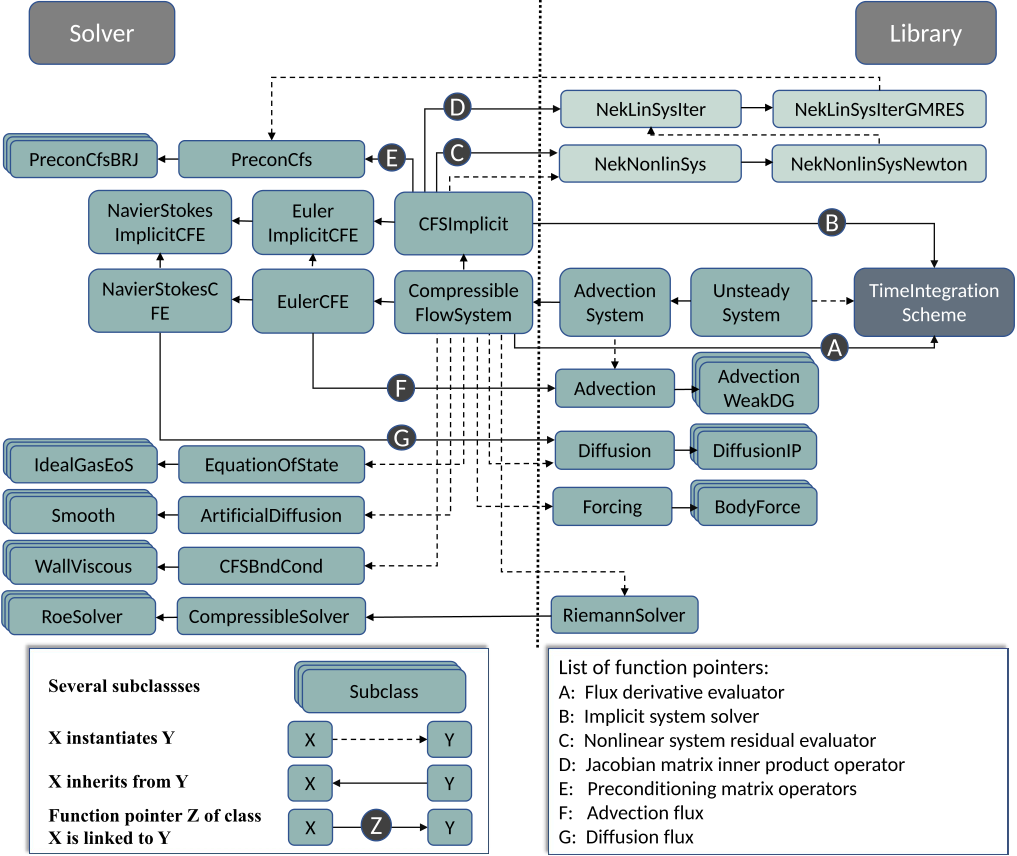
\includegraphics[width=1\textwidth]{./img/DataStructureFinal}
        \par\end{centering}
    \centering{}\caption{Class structure of the explicit and implicit solvers. The equation system classes ($\texttt{ EulerCFE}$ or $\texttt{ NavierStokesCFE}$) contain access to the main functionalities of the solver, such as time integration, and the solution fields. They make use of numerical methods from the libraries, such as $\texttt{ AdvectionWeakDG}$, and equations system related functions, such as the advection flux ($\texttt{ F}$) and diffusion flux ($\texttt{ G}$), to form the spatial discretization operator $\texttt{ A}$. The spatial operator $\texttt{ A}$ and the time integration method form the explicit solver using the method of lines. For the implicit solver, additional classes like the Newton solver ($\texttt{ NekNonlinSysNewton}$), GMRES solver ($\texttt{ NekLinSysIterGMRES}$) and linear algebra solver of preconditioners (e.g. $\texttt{ PrecondCfsBRJ}$) are instantiated. Together with operators related to the nonlinear system ($\texttt{ C}$), the Jacobian matrix ($\texttt{ D}$) and preconditioning matrix ($\texttt{ E}$), an implicit system solver ($\texttt{ B}$) is constructed, which is linked to the implicit time integration scheme to form the implicit solver.} \label{fig:Class-structure-of}
  \end{figure}
  

  The main procedures for building a solver are briefly introduced using
  the explicit solver of the NS equations as an example. Besides the main
  solver class ($\texttt{ CompressibleFlowSolver}$) which controls the
  solving procedure, an equation system class is needed. The
  equation system classes ($\texttt{ EulerCFE}$ or $\texttt{ NavierStokesCFE}$)
  are instantiated and initialized dynamically based on user inputs using
  a factory method pattern \cite{Cantwell2015}, which is also extensively
  used for the dynamic object creation of classes in the solver. The equation
  system class inherits instantiations of classes related to geometry
  information, solution approximation, time integration and others from
  equations system classes in the libraries such as $\texttt{ UnsteadySystem}$
  in $\texttt{ SolverUtils}$. Thus the main functionality of the equation system class
  is to offer equation system related functions and to form spatial
  discretization operators using numerical methods from the libraries
  such as, $\texttt{ AdvectionWeakDG}$. Fig.~\ref{fig:Class-structure-of}
  illustrates the class structure of the explicit and implicit solvers.
  The equation of state ($\texttt{ EquationOfState}$), boundary conditions
  ($\texttt{ CFSBndCond}$), Riemann flux ($\texttt{ RiemmanSolver}$), shock
  capturing method ($\texttt{ ArtificialDiffusion}$), forcing term ($\texttt{ Forcing}$),
  advection flux (function pointer $\texttt{ F}$) and diffusion flux (function
  pointer $\texttt{ G}$) are instantiated or implemented in the equation system class.
  Specific numerical schemes like the weak
  DG scheme for advection terms ($\texttt{ AdvectionWeakDG}$) and the interior
  penalty method for diffusion terms ($\texttt{ DiffusionIP}$) are instantiated
  to calculate $\mathbf{\nabla}\cdot\mathbf{F}$
  and $\mathbf{\nabla}\cdot\mathbf{G}$ in Eq. \eqref{eq:NS-Eqs}
  provided with all these equation system related functions ($\texttt{ F}$ and $\texttt{ G}$). Finally
  the spatial discretization operator $\textit{L}_{\delta}\left(\mathbf{u},t\right)$
  is linked to the time integration class using the pointer-to-function
  $\texttt{ A}$ and the explicit solver is complete.

  The main simulation flowchart of the implicit solver is given in Tab. \ref{tab:Cfs-NSFlow-chart}, which also shows the flow between different classes.
  \begin {table}[htbp!]
    \caption {Nassi--Shneiderman diagram of the implicit solver with the corresponding
    class names. Brown: library class ; cyan: solver class.} \label{tab:Cfs-NSFlow-chart} 
  \begin{tabular}{|l|l|l|l|l|l||ll||l||l||l||l||l|}
    \hline 
    \multicolumn{7}{|l}{Initialization} & \multicolumn{6}{l|}{{\footnotesize{}in }\textcolor{cyan}{\footnotesize{}$\texttt{CompressibleFlowSolver}$}}\tabularnewline
    \hline 
    \multicolumn{7}{|l}{Time step loop $n$} & \multicolumn{6}{l|}{{\footnotesize{}in }\textcolor{brown}{\footnotesize{}$\texttt{UnsteadySystem}$}}\tabularnewline
    \cline{2-13} \cline{3-13} \cline{4-13} \cline{5-13} \cline{6-13} \cline{7-13} \cline{8-13} \cline{9-13} \cline{10-13} \cline{11-13} \cline{12-13} \cline{13-13} 
    \multirow{12}{*}{} & \multicolumn{6}{l}{Runge-Kutta loop $m=1,\cdots,M$} & \multicolumn{6}{l|}{{\footnotesize{}in }\textcolor{brown}{\footnotesize{}$\texttt{TimeIntegrationScheme}$}}\tabularnewline
    \cline{3-13} \cline{4-13} \cline{5-13} \cline{6-13} \cline{7-13} \cline{8-13} \cline{9-13} \cline{10-13} \cline{11-13} \cline{12-13} \cline{13-13} 
     & \multirow{10}{*}{} & \multicolumn{5}{l}{Calculate source term $\mathbf{S}_{m}$} & \multicolumn{6}{l|}{{\footnotesize{}in }\textcolor{brown}{\footnotesize{}$\texttt{TimeIntegrationScheme}$}}\tabularnewline
    \cline{3-13} \cline{4-13} \cline{5-13} \cline{6-13} \cline{7-13} \cline{8-13} \cline{9-13} \cline{10-13} \cline{11-13} \cline{12-13} \cline{13-13} 
     &  & \multicolumn{5}{l}{Netwon iteration $l$} & \multicolumn{6}{l|}{{\footnotesize{}in }\textcolor{brown}{\footnotesize{}$\texttt{NewtonSolver}$}}\tabularnewline
    \cline{4-13} \cline{5-13} \cline{6-13} \cline{7-13} \cline{8-13} \cline{9-13} \cline{10-13} \cline{11-13} \cline{12-13} \cline{13-13} 
     &  & \multirow{8}{*}{} & \multicolumn{4}{l}{Calculate residual $\mathbf{N}\left(\bar{\mathbf{u}}^{l}\right)$} & \multicolumn{6}{l|}{{\footnotesize{}in }\textcolor{cyan}{\footnotesize{}$\texttt{CFSImplicit}$}}\tabularnewline
    \cline{4-13} \cline{5-13} \cline{6-13} \cline{7-13} \cline{8-13} \cline{9-13} \cline{10-13} \cline{11-13} \cline{12-13} \cline{13-13} 
     &  &  & \multicolumn{4}{l}{GMRES iteration $k$} & \multicolumn{6}{l|}{{\footnotesize{}in }\textcolor{brown}{\footnotesize{}$\texttt{NekLinSysIterGMRES}$}}\tabularnewline
    \cline{5-13} \cline{6-13} \cline{7-13} \cline{8-13} \cline{9-13} \cline{10-13} \cline{11-13} \cline{12-13} \cline{13-13} 
     &  &  & \multirow{5}{*}{} & \multicolumn{3}{l}{Calculate search vector $\mathbf{q}_{k}$} & \multicolumn{6}{l|}{{\footnotesize{}in }\textcolor{brown}{\footnotesize{}$\texttt{NekLinSysIterGMRES}$}}\tabularnewline
    \cline{5-13} \cline{6-13} \cline{7-13} \cline{8-13} \cline{9-13} \cline{10-13} \cline{11-13} \cline{12-13} \cline{13-13} 
     &  &  &  & \multicolumn{3}{l}{BRJ iteration $j=1,\cdots,J$ } & \multicolumn{6}{l|}{{\footnotesize{}in }\textcolor{brown}{\footnotesize{}$\texttt{PrecondBRJ}$}}\tabularnewline
    \cline{6-13} \cline{7-13} \cline{8-13} \cline{9-13} \cline{10-13} \cline{11-13} \cline{12-13} \cline{13-13} 
     &  &  &  &  & \multicolumn{2}{l}{Calculate {\small{}$\hat{\mathbf{q}}^{j}=\hat{\mathbf{D}}^{-1}\left(\mathbf{q}_{k}-\left(\mathbf{\hat{L}}+\hat{\mathbf{U}}\right)\hat{\mathbf{q}}^{j-1}\right)$}} & \multicolumn{6}{l|}{{\footnotesize{}in }\textcolor{cyan}{\footnotesize{}$\texttt{CFSImplicit}$}}\tabularnewline
    \cline{5-13} \cline{6-13} \cline{7-13} \cline{8-13} \cline{9-13} \cline{10-13} \cline{11-13} \cline{12-13} \cline{13-13} 
     &  &  &  & \multicolumn{3}{l}{Calculate $\partial\mathbf{N}/\partial\mathbf{u}\cdot\hat{\mathbf{q}}^{J}$} & \multicolumn{6}{l|}{{\footnotesize{}in }\textcolor{cyan}{\footnotesize{}$\texttt{CFSImplicit}$}}\tabularnewline
    \cline{5-13} \cline{6-13} \cline{7-13} \cline{8-13} \cline{9-13} \cline{10-13} \cline{11-13} \cline{12-13} \cline{13-13} 
     &  &  &  & \multicolumn{3}{l}{Calculate linear system residual} & \multicolumn{6}{l|}{{\footnotesize{}in }\textcolor{brown}{\footnotesize{}$\texttt{NekLinSysIterGMRES}$}}\tabularnewline
    \cline{4-13} \cline{5-13} \cline{6-13} \cline{7-13} \cline{8-13} \cline{9-13} \cline{10-13} \cline{11-13} \cline{12-13} \cline{13-13} 
     &  &  & \multicolumn{4}{l}{Calculate $\bar{\mathbf{u}}^{l+1}$ by linear combination of $\mathbf{q}_{k}$} & \multicolumn{6}{l|}{{\footnotesize{}in }\textcolor{brown}{\footnotesize{}$\texttt{NekLinSysIterGMRES}$}}\tabularnewline
    \cline{2-13} \cline{3-13} \cline{4-13} \cline{5-13} \cline{6-13} \cline{7-13} \cline{8-13} \cline{9-13} \cline{10-13} \cline{11-13} \cline{12-13} \cline{13-13} 
     & \multicolumn{6}{l}{Calculate $\mathbf{u}^{n+1}$} & \multicolumn{6}{l|}{{\footnotesize{}in }\textcolor{brown}{\footnotesize{}$\texttt{TimeIntegrationScheme}$}}\tabularnewline
    \hline 
    \multicolumn{7}{|l}{Output and finalization} & \multicolumn{6}{l|}{{\footnotesize{}in }\textcolor{cyan}{\footnotesize{}$\texttt{CompressibleFlowSolver}$}}\tabularnewline
    \hline 
    \end{tabular}
  \end{table}

   %% \begin{figure}
   %%        \caption{CompressibleFlowSolver Main Flow Chart}
   %%      \centering
   %%    \begin{tikzpicture}[scale=0.2,node distance=1cm]
   %%    \node (A)
   %%    [rectangle,
   %%    rounded corners,
   %%    minimum width=8cm,
   %%    minimum height=1cm,
   %%    text centered,
   %%    draw=black,
   %%    fill=red!30]
   %%    {CompressibleFlowSolver$.$cpp};
   %%    \node (B_1)
   %%    [rectangle,
   %%    rounded corners,
   %%    minimum width=8cm,
   %%    minimum height=1cm,
   %%    text width=8cm,
   %%    text centered,
   %%    draw=black,
   %%    fill=blue!20,
   %%    below =of A,
   %%    xshift=0cm,
   %%    yshift=0cm]
   %%    {Initialize Objects\\eg. DriverStandard::v$\_$InitObject\\See Figure \ref{fig1}};
   %%    \draw[arrow](A)--(B_1);
   %%    \node (B_2)
   %%    [rectangle,
   %%    rounded corners,
   %%    minimum width=8cm,
   %%    minimum height=1cm,
   %%    text width=8cm,
   %%    text centered,
   %%    draw=black,
   %%    fill=blue!20,
   %%    below =of B_1,
   %%    xshift=0cm,
   %%    yshift=0cm]
   %%    {Execute Solver beginning from driver:\\eg. DriverStandard::v$\_$Execute};
   %%    \draw[arrow](B_1)--(B_2);
   %%    \node (C_1)
   %%    [rectangle,
   %%    rounded corners,
   %%    minimum width=8cm,
   %%    minimum height=1cm,
   %%    text width=8cm,
   %%    text centered,
   %%    draw=black,
   %%    fill=yellow!20,
   %%    right= of B_2,
   %%    xshift=0cm,
   %%    yshift=0cm]
   %%    {Initial conditions: \\m$\_$equ[0]-$>$DoInitialise\\ See Figure \ref{fig2}};
   %%    \draw[arrow](B_2.east)--(C_1);
   %%    \node (C_2)
   %%    [rectangle,
   %%    rounded corners,
   %%    minimum width=8cm,
   %%    minimum height=1cm,
   %%    text width=8cm,
   %%    text centered,
   %%    draw=black,
   %%    fill=yellow!20,
   %%    below = of C_1,
   %%    xshift=0cm,
   %%    yshift=0cm]
   %%    {Main execution of solver:\\m$\_$equ[0]-$>$DoSolve\\ See Figure \ref{fig3} and Figure \ref{fig4}};
   %%    \draw[arrow](B_2.east)--($(B_2.east)+(2cm,0)$)|-(C_2);
   %%    \node (C_3)
   %%    [rectangle,
   %%    rounded corners,
   %%    minimum width=8cm,
   %%    minimum height=1cm,
   %%    text width=8cm,
   %%    text centered,
   %%    draw=black,
   %%    fill=yellow!20,
   %%    below = of C_2,
   %%    xshift=0cm,
   %%    yshift=0cm]
   %%    {Output brief information:\\m$\_$equ[0]-$>$Output};
   %%    \draw[arrow](B_2.east)--($(B_2.east)+(2cm,0)$)|-(C_3);
   %%    \end{tikzpicture}
   %%  \end{figure}
    

%% \clearpage
%%    \begin{figure}
%%           \caption{CompressibleFlowSolver InitObject}\label{fig1}
%%         \centering
%%         \includestandalone[width=1\linewidth]{FlowChart1}
%%     \end{figure}

%% \clearpage
%%    \begin{figure}
%%           \caption{CompressibleFlowSolver Initialize Conditions}\label{fig2}
%%         \centering
%%         \includestandalone[width=1\linewidth]{FlowChart2}
%%     \end{figure}

%% \clearpage
%%    \begin{figure}
%%           \caption{CompressibleFlowSolver Execute Advection}\label{fig3}
%%         \centering
%%         \includestandalone[width=0.5\linewidth]{FlowChart3}
%%    \end{figure}

%% \clearpage
%%    \begin{figure}
%%           \caption{CompressibleFlowSolver Execute Diffusion}\label{fig4}
%%         \centering
%%         \includestandalone[width=0.5\linewidth]{FlowChart4}
%%    \end{figure}


% \section{The Fundamentals Behind the Compressible Flow Solver}

% \subsection{Strong Form of the System}

% \subsection{Variational Form of the System}

% \section{The Fundamentals Behind the Data Structures}

% \subsection{Overview}

% \subsection{Equation System Description}

% \subsection{Advection Components}

% \subsection{Diffusion Components}


% \section{The Fundamental Flow Control of The Solver: Flow Chart}

% \subsection{Top-Down Perspective}

% \subsection{Evaluation of the Explicit Term}

% \subsection{Evaluation of the Implicit Term}

% \section{The Fundamental Algorithms}

% \paragraph{How Would I Change From External Energy Form to Internal Energy Form?}

% \paragraph{How Is De-Aliasing Applied to the Non-Linear Terms?}



%%%%%%%%%%%%%%%%%%%%%%%%%%%%%%%


%%
\part{Utilities} \label{part:utilities}

% Utilities Master File

In this part of the developer's guide, we walk you through development aspects of the various utilities that are available within publicly-available \nek repository.
We encourage you to incorporate these utilities into your science and engineering work flows.  If you find that the current utilities do not meet your needs and consequently you end up building
a new utility based upon our framework, we encourage you to consider submitting this to us for incorporation in the publicly-available master branch.


%%%%%%%%%%%%%%%%%%%%%%%%%%%%%%%
\chapter{FieldConvert}

In this chapter, we walk the reader through FieldConvert.



%%%%%%%%%%%%%%%%%%%%%%%%%%%%%%%
\chapter{NekMesh}

In this chapter, we walk the reader through NekMesh.




\part{NekPy: Python interface to \nek{}} \label{part:nekpy}

\chapter{Introduction}

This part of the guide contains the information on using and developing \texttt{NekPy} 
Python wrappers for the \nek{} spectral/\textit{hp} element framework. 
\emph{As a disclaimer, these wrappings are experimental and incomplete.} 
You should not rely on their current structure and API remaining unchanged.

Currently, representative classes from the \texttt{LibUtilities}, \texttt{StdRegions},
\texttt{SpatialDomains}, \texttt{LocalRegions} and \texttt{MultiRegions} libraries 
have been wrapped in order to show the proof-of-concept.

\section{Features and functionality}

\texttt{NekPy} uses the \texttt{Boost.Python} library to provide a set of high-quality,
hand-written Python bindings for selected functions and classes in Nektar++. 

It is worth noting that Python (CPython, the standard Python implementation written in C, 
in particular) includes C API and that everything in Python is strictly speaking a C 
structure called \texttt{PyObject}. Hence, defining a new class, method etc. in Python 
is in reality creating a new \texttt{PyObject} structure.

Boost.Python is essentially a wrapper for Python C API which conveniently exports C++ 
classes and methods into \texttt{PyObjects}. At compilation time a dynamic library 
is created which is then imported to Python, as shown in Figure \ref{fig:boost_python}. 

\begin{figure}[h!]
	\centering
    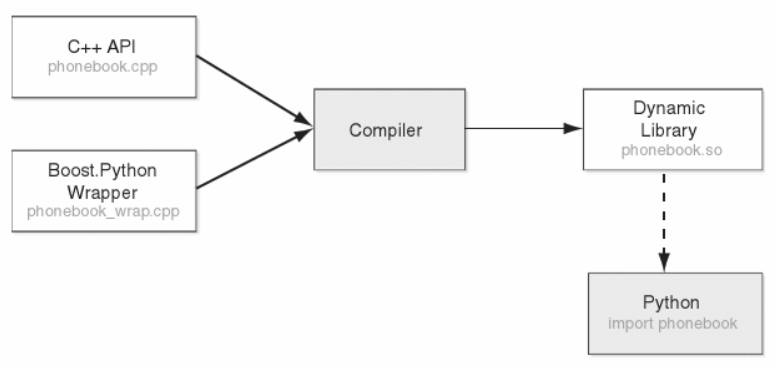
\includegraphics[width=0.9\textwidth]{img/boost_python}
    \caption{A schematic diagram of how C++ code is converted into Python with Boost.Python \cite{C++Api}}
    \label{fig:boost_python}
\end{figure}

A typical snippet could look something like:

\begin{lstlisting}[caption={NekPy sample snippet}, label={lst:nekpy_sample}, language=Python]
from NekPy.LibUtilities import PointsKey, PointsType, BasisKey, BasisType
from NekPy.StdRegions import StdQuadExp
import numpy as np
numModes = 8
numPts   = 9
ptsKey   = PointsKey(numPts, PointsType.GaussLobattoLegendre)
basisKey = BasisKey(BasisType.Modified_A, numModes, ptsKey)
quadExp  = StdQuadExp(basisKey, basisKey)
x, y     = quadExp.GetCoords()
fx       = np.sin(x) * np.cos(y)
proj     = quadExp.FwdTrans(fx)
\end{lstlisting}

\texttt{NekPy} uses the \texttt{Boost.NumPy} library, contained in Boost 1.63+, to
automatically convert C++ \texttt{Array<OneD, >} objects to and from the commonly-used
\texttt{numpy.ndarray} object, which makes the integration more seamless between Python
and C++.
\chapter{Installing NekPy}

NekPy has the following list of requirements:

\begin{itemize}
	\item Boost with Python support
	\item Nektar++ \texttt{master} branch compiled from source (i.e. not from packages)
	\item Python 2.7+ (note that examples rely on Python 2.7)
	\item NumPy
\end{itemize}

Most of these can be installed using package managers on various operating
systems, as we describe below. We also have a requirement on the \texttt{Boost.NumPy}
package, which is available in Boost 1.63 or later. If this isn't found on your
system, it will be automatically downloaded and compiled.

\section{Compiling and installing Nektar++}

Nektar++ should be compiled as per the user guide instructions and installed
into a directory which we will refer to as \texttt{\$NEKDIR}. By default this is the
\texttt{dist} directory inside the Nektar++ build directory.

Note that Nektar++ must, at a minimum, be compiled with \texttt{NEKTAR\_BUILD\_LIBRARY},
\texttt{NEKTAR\_BUILD\_UTILITIES} , \texttt{NEKTAR\_BUILD\_SOLVERS} and \texttt{NEKTAR\_BUILD\_PYTHON}. 
This will automatically download and install \texttt{Boost.NumPy} if required. Note 
that all solvers may be disabled as long as the \texttt{NEKTAR\_BUILD\_SOLVERS} option is set. 

\subsection{macOS}

\subsubsection{Homebrew}

Users of Homebrew should make sure their installation is up-to-date with 
\texttt{brew upgrade}. Then run

\begin{lstlisting}[language=bash]
brew install python boost-python
\end{lstlisting}

To install the NumPy package, use the \texttt{pip} package manager:

\begin{lstlisting}[language=bash]
pip install numpy
\end{lstlisting}

\subsubsection{MacPorts}

Users of MacPorts should sure their installation is up-to-date with 
\texttt{sudo port selfupdate \&\& sudo port upgrade outdated}. Then run

\begin{lstlisting}[language=bash]
sudo port install python27 py27-numpy
sudo port select --set python python27
\end{lstlisting}


\subsection{Linux: Ubuntu/Debian}

Users of Debian and Ubuntu Linux systems should sure their installation is
up-to-date with \texttt{sudo apt-get update \&\& sudo apt-get upgrade}

\begin{lstlisting}[language=bash]
sudo apt-get install libboost-python-dev python-numpy
\end{lstlisting}

\subsection{Compiling the wrappers}

Run the following command in \path{$NEKDIR/build} directory to install the Python package
for the current user:

\begin{lstlisting}[language=bash]
make nekpy-install-user
\end{lstlisting}

Alternatively, the following command can be used to install the package for all users:

\begin{lstlisting}[language=bash]
make nekpy-install-system
\end{lstlisting}


\section{Using the bindings}

By default, the bindings will install into the \texttt{dist} directory, along with a
number of examples that are stored in the 
\path{$NEKDIR/library/Demos/Python} directory. To 
test your installation, you can for example run one of these (e.g. \texttt{python Basis.py}) or
launch an interactive session:

\begin{lstlisting}[language=bash]
$ cd builds
$ python
Python 2.7.13 (default, Apr  4 2017, 08:47:57) 
[GCC 4.2.1 Compatible Apple LLVM 8.1.0 (clang-802.0.38)] on darwin
Type "help", "copyright", "credits" or "license" for more information.
>>> from NekPy.LibUtilities import PointsKey, PointsType
>>> PointsKey(10, PointsType.GaussLobattoLegendre)
<NekPy.LibUtilities._LibUtilities.PointsKey object at 0x11005c310>
\end{lstlisting}

\subsection{Examples}

A number of examples of the wrappers can be found in the 
\path{$NEKDIR/library/Demos/Python}
directory, along with a sample mesh \texttt{newsquare\_2x2.xml}:

\begin{itemize}
	\item \texttt{SessionReader.py} is the simplest example and shows how to construct a
  		session reader object. Run it as \texttt{python SessionReader.py mesh.xml}.
  	\item \texttt{Basis.py} shows functionality of basic \texttt{LibUtilities} points and basis
  		classes. Run this as \texttt{python Basis.py}.
	\item \texttt{StdProject.py} shows how to use some of the \texttt{StdRegions} wrappers and
  		duplicates the functionality of \texttt{Basis.py} using the \texttt{StdExpansion} class. Run
  		this as \texttt{python StdProject.py}.
	\item \texttt{MeshGraph.py} loads a mesh and prints out some basic properties of its
		quadrilateral elements. Run it as \texttt{python MeshGraph.py newsquare\_2x2.xml}.
\end{itemize}

If you want to modify the source files, it's advisable to edit them in the
\path{$NEKDIR/library/Demos/Python} directory and 
re-run \texttt{make install}, otherwise local changes will be overwritten by the next \texttt{make install}.

\chapter{Package structure}

The NekPy wrapper is designed to mimic the library structure of Nektar++, with
directories for the \texttt{LibUtilities}, \texttt{SpatialDomains} and
\texttt{StdRegions} libraries. This is a deliberate design decision, so that
classes and definitions in Nektar++ can be easily located inside NekPy.

There are also some other directories and files:

\begin{itemize}
  \item \path{LibUtilities/Python/NekPyConfig.hpp} is a convenience header that
  all \texttt{.cpp} files should import. It sets appropriate namespaces and
  defines commonly used macros.
  \item \path{cmake/python} contains templates for \texttt{init.py} and
  \texttt{setup.py} files which every Python package should contain,
  \item \path{cmake/ThirdPartyPython.cmake} is a CMake configuration file which
  searches for Python and prepares \texttt{make} targets for installing NekPy.
\end{itemize}

Figure \ref{fig:package_str} shows the location of Python wrapper files within
Nektar++ structure.  Every sub-module of Nektar++ hosts an additional folder for
Python files and the structure of the Python folder mimics the structure of the
sub-module itself, as shown on the left of the figure with \texttt{LibUtilities}
sub-module. Individual \texttt{.cpp} files, such as \texttt{Expansion.cpp}
contain the wrappers for classes and methods from corresponding Nektar++ library
files whereas \texttt{.cpp} files named after sub-modules
(e.g. \texttt{LibUtilities.cpp}) contain \texttt{PYBIND11\_MODULE} definitions
which create package modules (e.g. \texttt{NekPy.LibUtilities}).

\begin{figure}[h!]
  \centering
  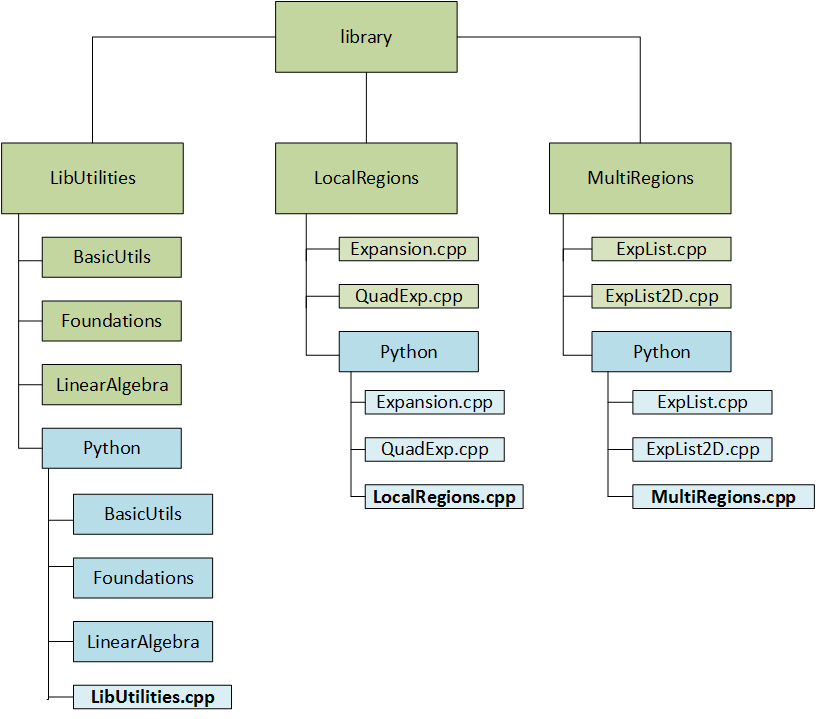
\includegraphics[width=0.9\textwidth]{img/package_str}
  \caption{The location of Python wrapper files within Nektar++ structure.}
  \label{fig:package_str}
\end{figure}

\chapter{NekPy wrapping guide}

This section attempts to outline some of the basic principles of the NekPy
wrapper, which relies entirely on the excellent \texttt{pybind11} library. An
extensive documentation is therefore beyond the scope of this document, but we
highlight aspects that are important for the NekPy wrappers.

In general, note that when things go wrong with \texttt{pybind11}, it'll be
indicated either by an extensive compiler error, or a runtime error in the
Python interpreter when you try to use your wrapper. Judicious use of Google is
therefore recommended to track down these issues!

You may also find the following resources useful:

\begin{itemize}
  \item \href{https://pybind11.readthedocs.io/en/stable/basics.html}{The \texttt{pybind11} tutorial};
  \item \href{https://pybind11.readthedocs.io/en/stable/index.html}{The \texttt{pybind11} documentation}.
\end{itemize}

To demonstrate how to wrap classes, we'll refer to a number of existing parts of
the code below.

\section{Defining a library}

First consider \texttt{LibUtilities}. An abbreviated version of the base file,
\texttt{LibUtilities.cpp} has the following structure:

\begin{lstlisting}[caption={Defining a library with pybind11}, label={lst:defining_a_library}, language=C++]
#include <LibUtilities/Python/NekPyConfig.hpp>

void export_Basis(py::module &);
void export_SessionReader(py::module &);

// Define the LibUtilities module within the pybind11 module `m`.
PYBIND11_MODULE(_LibUtilities, m)
{
    // Export classes.
    export_Basis(m);
    export_SessionReader(m);
}
\end{lstlisting}

The \texttt{PYBIND11\_MODULE(name, m)} macro allows us to define a Python module
inside C++. Note that in this case, the leading underscore in the name
(i.e. \texttt{\_LibUtilities}) is deliberate. To define the contents of the module,
we call a number of functions that are prefixed by \texttt{export\_}, which will
define one or more Python classes that live in this module. These Python classes
correspond with our Nektar++ classes. We adopt this approach simply so that we
can split up the different classes into different files, because it is not
possible to call \texttt{PYBIND11\_MODULE} more than once.

These functions are defined in appropriately named files, for example
\texttt{export\_Basis()} lives in the file
\path{LibUtilities/Python/Foundations/Basis.cpp}. This corresponds to the
Nektar++ file \path{LibUtilities/Foundations/Basis.cpp} and the classes defined
therein.

\section{Basic class wrapping}

As a very basic example of wrapping a class, let's consider a minimal wrapper
for \texttt{SessionReader}:

\begin{lstlisting}[caption={Basic class wrapping with \texttt{pybind11}}, label={lst:basic_class_wrapping}, language=C++]
void export_SessionReader(py::module &m)
{
  py::class_<SessionReader, std::shared_ptr<SessionReader>>(
      m, "SessionReader")

    .def_static("CreateInstance", SessionReader_CreateInstance)

    .def("GetSessionName", &SessionReader::GetSessionName,
         py::return_value_policy::copy)

    .def("InitSession", &SessionReader::InitSession,
         py::arg("filenames") = py::list())

    .def("Finalise", &SessionReader::Finalise)
    ;
}
\end{lstlisting}

\subsection{\texttt{py::class\_<>}}

This \texttt{pybind11} object defines a Python class in C++. It is templated,
and in this case we have the following template arguments:

\begin{itemize}
  \item \texttt{SessionReader} is the class that will be wrapped;
  \item \texttt{std::shared\_ptr<SessionReader>} indicates that this object
  should be stored inside a shared (or smart) pointer, which we frequently use
  throughout the library, as can be seen by the frequent use of
  \texttt{SessionReaderSharedPtr}.
\end{itemize}

We then have two arguments:

\begin{itemize}
  \item \texttt{m} is the module we are going to define the class within.
  \item \texttt{"SessionReader"} is the name of the class in Python.
\end{itemize}

\subsection{Wrapping member functions}

We then call the \texttt{.def} function on the \texttt{class\_<>}, which allows
us to define member functions on our class. This is equivalent to
\texttt{def}-ing a function in Python. \texttt{.def} has two required
parameters, and one optional parameter:

\begin{itemize}
  \item The function name as a string, e.g. \texttt{"GetSessionName"}
  \item A function pointer that defines the C++ function that will be called
  \item An optional return policy, which we need to define when the C++ function
  returns a reference.
\end{itemize}

\texttt{pybind11} is very smart and can convert many Python objects to their
equivalent C++ function arguments, and C++ return types of the function to their
respective Python object. Many times therefore, one only needs to define the
\texttt{.def()} call.

However, there are some instances where we need to do some additional
conversion, mask some C++ complexity from the Python interface, or deal with
functions that return references. We describe ways to deal with this below.

\subsubsection{Thin wrappers}

Instead of defining a function pointer to a member of the C++ class, we can
define a function pointer to a separate function that defines some extra
functionality. This is called a \emph{thin wrapper}.

As an example, consider the \texttt{CreateInstance} function. In C++ we pass
this function the command line arguments in the usual \texttt{argc},
\texttt{argv} format. In Python, command line arguments are defined as a list of
strings inside \texttt{sys.argv}. However, \texttt{pybind11} does not know how to
convert this list to \texttt{argc, argv}, so we need some additional code.

\begin{lstlisting}[caption={Thin wrapper example}, label={lst:thin_wrapper}, language=C++]
SessionReaderSharedPtr SessionReader_CreateInstance(py::list &ns)
{
    // ... some code here that converts a Python list to the standard
    // c/c++ (int argc, char **argv) format for command line arguments.
    // Then use this to construct a SessionReader and return it.
    SessionReaderSharedPtr sr = SessionReader::CreateInstance(argc, argv);
    return sr;
}
\end{lstlisting}

In Python, we can then simply call \texttt{session = SessionReader.CreateInstance(sys.argv)}.

\subsubsection{Dealing with references}

When dealing with functions in C++ that return references, e.g. \texttt{const
  NekDouble \&GetFactor()} we need to supply an additional argument to
\texttt{.def()}, since Python immutable types such as strings and integers
cannot be passed by reference. There are also lifetime implications; i.e. if the
C++ object being referenced is destroyed whilst still being used in Python, this
would cause the program to abort.

To address this, we can define a \emph{return value policy} which allows
\texttt{pybind11} to take various actions based on the intent of the
function. For a full list of options, consult the \texttt{pybind11]} guide on
\href{https://pybind11.readthedocs.io/en/stable/advanced/functions.html#return-value-policies}{return
  value policies}. However in this case we opt to use \texttt{copy} as
highlighted above, which will create a copy of the const reference and return
this to Python, thereby avoiding any lifetime issues.

\subsubsection{Dealing with \texttt{Array<OneD, >}}

The \path{LibUtilities/Python/BasicUtils/SharedArray.cpp} file contains a number
of functions that allow for the automatic conversion of Nektar++
\texttt{Array<OneD, >} storage to and from NumPy \texttt{ndarray} objects. This
means that you can wrap functions that take these as parameters and return
arrays very easily. However bear in mind the following caveats:

\begin{itemize}
  \item Any NumPy \texttt{ndarray} created from an \texttt{Array<OneD, >} (and
  vice versa) will share their memory. Although this avoids expensive memory
  copies, it means that changing the C++ array changes the contents of the NumPy
  array (and vice versa).
  \item Many functions in Nektar++ return Arrays through argument parameters. In
  Python this is a very unnatural way to write functions. For example:
  \begin{lstlisting}[language=Python]
    # This is good
    x, y, z = exp.GetCoords()
    # This is bad
    x, y, z = np.zeros(10), np.zeros(10), np.zeros(10)
    exp.GetCoords(x,y,z)
    # After this point x, y and z are updated as a result of GetCoords().
  \end{lstlisting}
  Use thin wrappers to overcome this problem. For examples of how to do this,
  particularly in returning tuples, consult the
  \texttt{StdRegions/StdExpansion.cpp} wrapper which contains numerous examples.
  \item \texttt{TwoD} and \texttt{ThreeD} arrays are not supported.
\end{itemize}

More information on the memory management and how the memory is shared can be
found in Section~\ref{sec:nekpy:memory}.

\subsection{Inheritance}

Nektar++ makes heavy use of inheritance, which can be translated to Python quite
easily using \texttt{pybind11}. For a good example of how to do this, you can
examine the \texttt{StdRegions} wrapper for \texttt{StdExpansion} and its
elements such as \texttt{StdQuadExp}. In a cut-down form, these look like the
following:

\begin{lstlisting}[caption={Inheritance with pybind11}, label={lst:inheritance}, language=C++]
void export_StdExpansion(py::module &m)
{
    py::class_<StdExpansion, std::shared_ptr<StdExpansion>>(m, "StdExpansion");
}
void export_StdQuadExp(py::module &m)
{
    py::class_<StdQuadExp, StdExpansion, std::shared_ptr<StdQuadExp>>(
        m, "StdQuadExp", py::multiple_inheritance())
        .def(py::init<const LibUtilities::BasisKey &,
                      const LibUtilities::BasisKey &>());
}
\end{lstlisting}

Note the following:

\begin{itemize}
  \item \texttt{StdExpansion} is an abstract class, so it has no initialiser and
  is non-copyable.
  \item We write the parent classes of \texttt{StdQuadExp} in the call to
  \texttt{class\_}. Note that this does not necessarily need to include the full
  hierarchy of C++ inheritance: in \texttt{StdRegions} the inheritance graph for
  \texttt{StdQuadExp} looks like \texttt{StdExpansion -> StdExpansion2D ->
    StdQuadExp}. In the above wrapper, we omit the \texttt{StdExpansion2D}
  reference entirely. However, in order to do skip classes in the inheritance
  tree, we need to tell \texttt{pybind11} about this by passing the
  \texttt{py::multiple\_inheritance} argument to the object.
  \item \texttt{py::init<>} is used to show how to wrap a C++ constructor. This
  can accept any arguments for which you have either written explicit wrappers
  or \texttt{pybind11} already knows how to convert.
\end{itemize}

\subsection{Wrapping enums}

Most Nektar++ enumerators come in the form:

\begin{lstlisting}[language=C++]
enum MyEnum {
    eItemOne,
    eItemTwo,
    SIZE_MyEnum
};
static const char *MyEnumMap[] = {
    "ItemOne"
    "ItemTwo"
    "ItemThree"
};
\end{lstlisting}

To wrap this, you can use the \texttt{NEKPY\_WRAP\_ENUM} macro defined in
\texttt{NekPyConfig.hpp}, which in this case can be used as
\texttt{NEKPY\_WRAP\_ENUM(m, MyEnum, MyEnumMap)}. Note that if instead of
\texttt{const char *} the map is defined as a \texttt{const std::string}, you
can use the \texttt{NEKPY\_WRAP\_ENUM\_STRING} macro.

\chapter{Documentation}

The NekPy package certainly had to be documented in order to provide an easily
accessible information about the wrapped classes to both users and
developers. Ideally, the documentation should be:
\begin{itemize}
  \item easily readable by humans,
  \item accessible using Python's inbuilt \texttt{help} method,
  \item compatible with the existing Nektar++ doxygen-based documentation.
\end{itemize}

Traditionally, Python classes and functions are documented using a docstring --
a string occurring as the very first statement after the function or class is
defined. This string is then accessible as the \texttt{\_\_doc\_\_} attribute of
the function or class. The conventions associated with Python docstrings are
described in PEP 257 document \cite{PEP257}.

\texttt{pybind11} provides an easy way to include docstrings in the wrapped methods
and classes as shown in Listing \ref{lst:doc_example}. The included docstrings
will appear when Python \texttt{help} method is used.

\begin{lstlisting}[caption={Example of class and method documentation in pybind11}, label={lst:doc_example}, language=C++]
void export_Points(py::module &m)
{
	py::class_<PointsKey>(m, "PointsKey", 
        "Create a PointsKey which uniquely defines quadrature points.\n"
        "\n"
        "Args:\n"
        "\tnQuadPoints (integer): The number of quadrature points.\n"
        "\tpointsType (PointsType object): The type of quadrature points.")
            .def(py::init<const int, const PointsType&>())
            .def("GetNumPoints", &PointsKey::GetNumPoints,
            "Get the number of quadrature points in PointsKey.\n"
            "\n"
            "Args:\n"
            "\tNone\n"
            "Returns:\n"
            "\tInteger defining the number of quadrature points in PointsKey.")
}
\end{lstlisting}

In order to fully document the existing bindings a number of enumeration type
classes such as \texttt{PointsType} had to have docstrings included which proved
to be a challenge since \texttt{pybind11} does not provide a way to do
this. Instead a direct call to Python C API has to be made and the method
adapted from \cite{PythonEnumDocstring} was used, as shown in Listing
\ref{lst:enum_doc}. A downside of this solution is that it does requires the
developer to manually update the Python documentation if the enumeration type is
ever changed (e.g.  adding a new type of point) as the code does not
automatically gather information from the C++ class. In theory it could be
possible to create a Python script which would generate Python docstrings based
on the existing C++ documentation using regular expressions; however it would be
difficult to integrate this solution into the existing framework.

\begin{lstlisting}[caption={Code used to include dosctings in enumetation type classes - part of \texttt{NekPyConfig.hpp}}, label={lst:enum_doc}, language=C++]
#define NEKPY_WRAP_ENUM_STRING_DOCS(ENUMNAME,MAPNAME,DOCSTRING)    \
    {                                                              \
        py::enum_<ENUMNAME> tmp(#ENUMNAME);                        \
        for (int a = 0; a < (int)SIZENAME(ENUMNAME); ++a)          \
        {                                                          \
            tmp.value(MAPNAME[a].c_str(), (ENUMNAME)a);            \
        }                                                          \
        tmp.export_values();                                       \
        PyTypeObject * pto =                                       \
            reinterpret_cast<PyTypeObject*>(tmp.ptr());            \
        PyDict_SetItemString(pto->tp_dict, "__doc__",              \
            PyString_FromString(DOCSTRING));                       \
    }
\end{lstlisting}

There are many docstrings conventions that are popular in Python such as
Epytext, reST and Google therefore a choice had to be made as to which docstring
style to use. After considering the criteria which the documentation had to
fulfill it was decided to use Google Python Style \cite{PythonGoogle} as it is
highly readable by humans (and hence an excellent choice for documentation which
will be primarily accessible by Python \texttt{help} method) and can be used to
generate automated documentation pages with Sphinx (a tool for creating Python
documentation).

Unfortunately, it proved to be difficult to include the documentation of NumPy
package in the existing doxygen-based documentation due to the fact that the
docstrings are generated by \texttt{pybind11}.  It was decided that if the time
constraints of the project permit this problem could be resolved at a later date
and the possibility of accessing the documentation though inbuilt \texttt{help}
method was deemed sufficient.

\chapter{Memory management in NekPy}

One of the biggest technical challenges of the NekPy project was to ensure the appropriate 
memory management between Python and C++. The computations carried out in \nek{} are 
usually highly demanding on the machines they are run on, therefore any unnecessary data 
duplication or memory leaks would be detrimental to software performance.

This section outlines the basics of memory management in C++ and Python as well as the 
solutions devised to effectively use the resources when passing data between the different 
layers of the bindings.

\section{Memory management in C++ and Python}

\subsection{C++}

In C++ the memory used by the application is divided into five containers \cite{C++Memory}:
\begin{itemize}
    \item text segment -- containing the set of instructions for the program to execute;
    \item data segment -- containing static and global variables initialised with values, 
    e.g. \texttt{float pi = 3.14;} -- the size of the data segment is pre-determined at 
    the time of the compilation of the program and depends on the size of the variables 
    in the source code;
    \item bss (block started by symbol) segment -- containing static and global variables 
    not explicitly initialised with any value, e.g. \texttt{int n;} -- the size of the 
    data segment is pre-determined at the time of the compilation of the program and 
    depends on the size of the variables in the source code;
    \item stack -- a LIFO (last in, first out) structure containing the function calls 
    and variables intialised in the functions -- the size of the stack is pre-determined 
    at the time of compilation of the program and depends on the operating system and 
    development environment;
    \item heap -- containing all dynamically allocated memory (e.g. using instruction 
    \texttt{new} in C++).
\end{itemize}

The access to data on the heap is maintained by pointers which store the memory address of 
said data. If the pointer ceases to exist (e.g. because the function which contained it 
finished running and hence was taken off the stack) the programmer has no way of referencing 
the data on the heap again. The unused, inaccessible data will stay in the memory, consuming 
valuable resources if not properly deallocated using \texttt{delete} instruction. Issues may 
arise if the same memory address is held by two different pointers -- the deallocation of 
memory can render one of the pointers empty and possibly lead to errors.

In order to facilitate memory management, C++11 standard introduced shared pointers 
(\texttt{shared\_ptr}) \cite{C++SharedPtr}. Shared pointers maintain a reference counter 
which is increased when another shared pointer refers to the same memory address. The memory 
will only be deallocated when all shared pointers referencing the memory are destroyed, as shown 
in Figure \ref{fig:shared_ptr}.

\begin{figure}[h!]
    \centering
    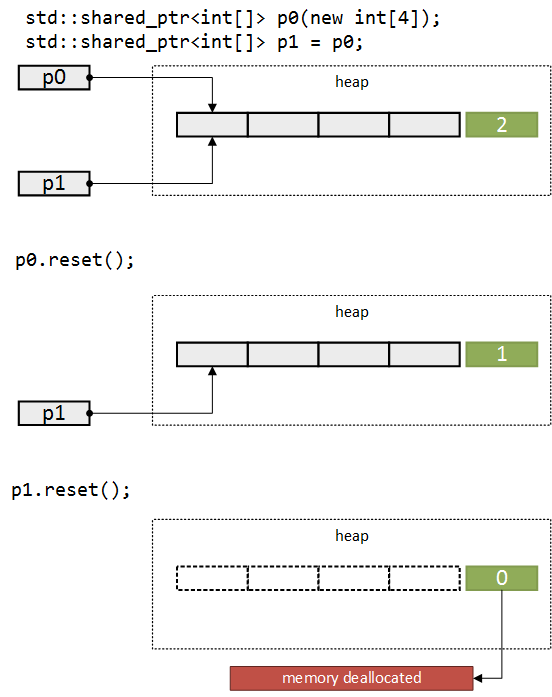
\includegraphics[width=0.6\textwidth]{img/shared_ptr}
    \caption{Memory management with C++11 \texttt{shared\_ptr}. The two declared shared pointers 
    reference an array of 4 integers. Reference counter shown in green.}
    \label{fig:shared_ptr}
\end{figure}

\subsubsection{Python}

Python manages memory though a private heap containing all Python objects \cite{PythonMemory}. 
An internal memory manager is used to ensure the memory is properly allocated and dealocated 
while the script runs. In contrast to C++, Python Memory Manager tries to optimise the memory 
usage as much as possible. For example, the same object reference is allocated to a new variable 
if the object already exists in memory. Another important feature of Python Memory Manager is 
the use of garbage collector based on reference counting. When the object is no longer referenced 
by any variable the reference counter is set to zero which triggers the garbage collector to free 
the memory. A disadvantage of this solution is slower execution time, since the garbage collector 
routines have to be called frequently. Features of Python Memory Manager are schematically shown 
in Figure \ref{fig:python_gc}

\begin{figure}[h!]
    \centering
    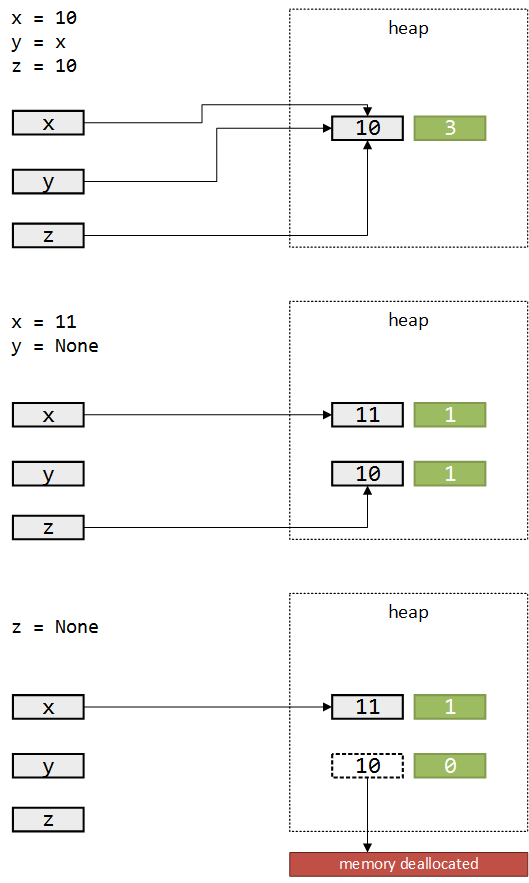
\includegraphics[width=0.6\textwidth]{img/python_gc}
    \caption{Memory management in Python. Memory is optimised as much as possible and garbage 
    collector deallocates the memory if the reference counter (shown in green) reaches 0.}
    \label{fig:python_gc}
\end{figure}

It is unusual for the Python programmer to manually modify the way Python uses memory resources 
-- however it is sometimes necessary, as is the case with this project. In particular, 
Python enables the programmer to increase or decrease the reference counter of the object 
using \texttt{Py\_XINCREF} and \texttt{Py\_XDECREF} respectively \cite{PythonManualMemory}.

\section{Passing C++ arrays to Python \footnote{The file implementing the below procedure: \texttt{LibUtilities\/Python\/LinearAlgebra\/NekMatrix.cpp}} }

In many situations arrays created by Nektar++ (usually a \texttt{shared\_ptr} of 
\texttt{NekMatrix<D, StandardMatrixTag>} type) in C++ need to be passed to Python - 
for instance, when preforming differentiation using e.g. Gauss quadrature rules a 
differentiation matrix must be obtained. In order to keep the program memory efficient 
the data should not be copied into a NumPy array but rather be referenced by the Python 
interface. This, however, complicates the issue of memory management.

Consider a situation, where C++ program no longer needs to work with the generated array 
and the memory dedicated to it is deallocated. Meanwhile, Python interface might still require 
the data contained within the array, only to be faced with an error as the data no longer 
exists in memory. To prevent such situations a solution employing reference counting must be used.

\subsubsection{Converter method}

Boost.Python provides the methods to do both convert a C++ type element to one recognised by 
Python as well as to maintain appropriate reference counting. Listing \ref{lst:c_to_python} 
shows an abridged version of the converter method (for Python 2 only) with comments on 
individual parameters. The object requiring conversion is a \texttt{shared\_ptr} of 
\texttt{NekMatrix<D, StandardMatrixTag>} type (named \texttt{mat}).

\begin{lstlisting}[caption={Converter method for converting the C++ arrays into Python NumPy arrays.}, label={lst:c_to_python}, language=C++]
#include <LibUtilities/LinearAlgebra/NekMatrix.hpp>
#include <LibUtilities/LinearAlgebra/MatrixStorageType.h>
#include <NekPyConfig.hpp>

using namespace Nektar;
using namespace Nektar::LibUtilities;

template<typename T, typename F>
void NekMatrixCapsuleDestructor(void *ptr) // destructor for the shared_ptr to data
{
    std::shared_ptr<NekMatrix<T, F>> *mat =
        (std::shared_ptr<NekMatrix<T, F>> *)ptr;
    delete mat;
}

template<typename T>
struct NekMatrixToPython
{
    static PyObject *convert(
        std::shared_ptr<NekMatrix<T, StandardMatrixTag>> const &mat)
    {
    py::object capsule(
            py::handle<>(PyCObject_FromVoidPtr(
                             new std::shared_ptr<NekMatrix<T, StandardMatrixTag>>(mat), // new shared_ptr to the data
                             NekMatrixCapsuleDestructor<T, StandardMatrixTag>))); // destructor method
                             
    int nRows = mat->GetRows(), nCols = mat->GetColumns();
    
    return py::incref( // increments Python reference counter
            np::from_data(
                mat->GetRawPtr(), // pointer to data
                np::dtype::get_builtin<T>(), // data type
                py::make_tuple(nRows, nCols), // shape of the array
                py::make_tuple(sizeof(T), nRows * sizeof(T)), // stride of the array
                capsule).ptr()); // capsule - contains the object owning the data (preventing it from being prematurely deallocated)
\end{lstlisting}

First, a new Python object is created, holding a shared pointer (\texttt{PyCObject\_FromVoidPtr}) 
to the array held in memory, increasing its reference counter and preventing it from being 
prematurely deallocated, as shown in Figure \ref{fig:c_to_python}, as well as destructor which 
contains instructions on what is to be done when the object is no longer needed (in this case, 
the \texttt{shared\_ptr} is to be deleted). It is worth noting that the steps (c) and (d) can 
be reversed and the \texttt{shared\_ptr} created by the Python binding can be removed first. 
In this case the memory will be deallocated only when the \texttt{shared\_ptr} created by C++ 
is also removed.

\begin{figure}[h!]
    \centering
    \begin{subfigure}{0.6\textwidth}
        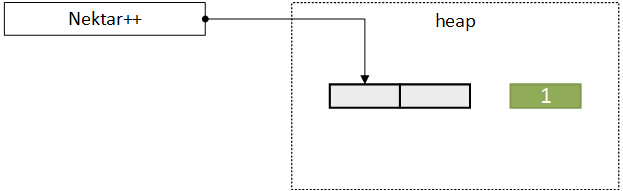
\includegraphics[width=0.99\textwidth]{c_to_python_a}
        \caption{Nektar++ creates a data array referenced by a \texttt{shared\_ptr}}
        \label{fig:c_to_python_a}
    \end{subfigure}
    \begin{subfigure}{0.6\textwidth}
        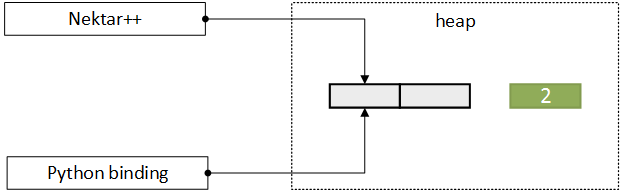
\includegraphics[width=0.99\textwidth]{c_to_python_b}
        \caption{Array is passed to Python binding which creates a new \texttt{shared\_ptr} 
        to the data}
        \label{fig:c_to_python_b}
    \end{subfigure}
    \begin{subfigure}{0.6\textwidth}
        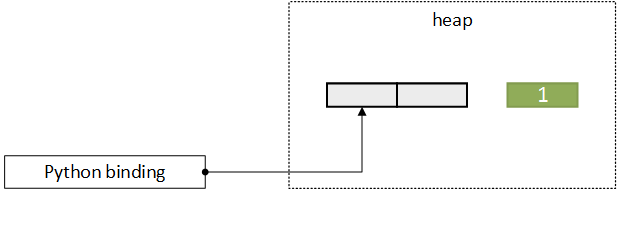
\includegraphics[width=0.99\textwidth]{c_to_python_c}
        \caption{Nektar++ no longer needs the data - its \texttt{shared\_ptr} is removed but 
        the memory is not deallocated}
        \label{fig:c_to_python_c}
    \end{subfigure}
    \begin{subfigure}{0.6\textwidth}
        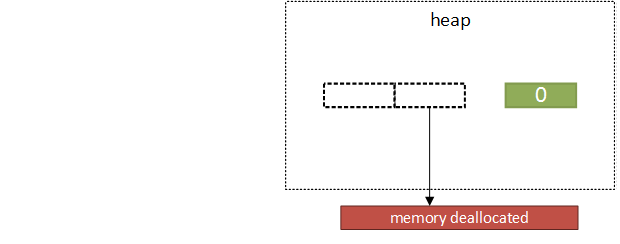
\includegraphics[width=0.99\textwidth]{c_to_python_d}
        \caption{When the data is no longer needed in the Python interface the destructor is 
        called and \texttt{shared\_ptr} is removed.}
        \label{fig:c_to_python_d}
    \end{subfigure}
    \caption{Memory management of data created in C++ using \texttt{shared\_ptr} and passed 
    to Python. Reference counter shown in green.}
    \label{fig:c_to_python}
\end{figure}

Then, a Boost.Python handle is created around the object, allowing Boost.Python to manage references 
correctly. Finally, a Boost.Python object named \texttt{capsule} is created from the handle.

The converter method returns a NumPy array -- this was chosen as it is a well-known datatype used 
in Python's popular \texttt{numpy} package. Additionally, Boost.Python allows the programmer to 
create a NumPy array from a generic C++ data container and to specify the owner of said container 
using the \texttt{np::from\_data} method. 

Care had to be taken to ensure that the array is presented in the correct order, especially as 
Nektar++ stores data in column major order whereas NumPy arrays are traditionally row major. 
The stride of the array has to be passed into the \texttt{np::from\_data} in a form of 
\texttt{(a, b)} tuple, where \texttt{a} is the number of bytes needed to skip to get to the 
same position in the next row and \texttt{b} is the number of bytes needed to skip to get to the 
same position in the next column. Hence, the tuple passed was \texttt{(sizeof(T), nRows * sizeof(T))}, 
where \texttt{T} is the datatype of the array.

In order to stop Python from immediately destroying the resulting NumPy array, its reference counter 
is manually increased before the array is passed on to Boost.Python and eventually returned to the user.

\subsubsection{Testing}

The process outlined above requires little manual intervention from the programmer. There are no almost 
no explicit calls to Python C API (aside from creating a \texttt{PyObject} -- \texttt{PyCObject\_FromVoidPtr}) 
as all operations are carried out by Boost.Python. Therefore, the testing focused mostly on correctness 
of returned data, in particular the order of the array.

To this end, the \emph{Differentiation} tutorials were used as tests. In order to correctly run the 
tutorials the Python wrapper needs to retrieve the differentiation matrix which, as mentioned before, 
has to be converted to a datatype Python recognises. The test runs the differentiation tutorials and 
compares the final result to the fixed expected value. The test is automatically run as a part of 
\texttt{ctest} command if both the Python wrapper and the tutorials have been built.

\subsection{Passing Python data to C++ 
\footnote{The files implementing the below procedure are: \texttt{LibUtilities/Python/BasicUtils/SharedArray.cpp} and \texttt{LibUtilities/BasicUtils/SharedArray.hpp}} }

Conversely, a similar problem exists when data is created in Python and has to be passed to 
the C++ program. In this case, as the data is managed by Python, the main reference counter 
should be maintained by the Python object and incremented or decremented as appropriate 
using \texttt{Py\_XINCREF} and \texttt{Py\_XDECREF} methods respectively.

When the array is no longer needed by the C++ program the reference counter on the Python 
side should be decremented in order for Python garbage collection to work appropriately 
-- however this should only happen when the array was created by Python in the first place. 

\subsubsection{Modifications to \texttt{Array<OneD, const DataType>} class template}

In order to perform the operations described above, the C++ array structure should contain 
information on whether or not it was created from data managed by Python. To this end, 
two new attributes were added to C++ \texttt{Array<OneD, const DataType>} class template:

\begin{itemize}
    \item \texttt{m\_memory\_pointer} - holding the pointer to the 
        \texttt{PyObject} containing the data,
    \item \texttt{m\_python\_decrement} - holding the pointer to the 
        callback function decrementing the reference counter of the \texttt{PyObject}.
\end{itemize}

If the two new attributes are not set to \texttt{nullptr} the array has been constructed 
throught the Python to C++ converter. The already existing \texttt{m\_count} attribute 
was retained in order to keep track of how many C++ references to the array there are.

Adding new attributes to the arrays might cause a significantly increased memory usage. 
Therefore a preprocessor directive has been added to only include the additional arguments 
if \texttt{NekPy} had been built (using the option \texttt{NEKTAR\_BUILD\_PYTHON}).

A new constructor has been added to the class template, as seen in Listing \ref{lst:new_const}. 
\texttt{m\_memory\_pointer} and \texttt{m\_python\_decrement} have been set to 
\texttt{nullptr} in the pre-existing constructors. A similar constructor was added for 
\texttt{const} arrays to ensure that these can also be passed between the languages. Note that 
no calls to Nektar++ array initialisation policies are made in this constructor, unlike in 
the pre-existing ones, as there is no need for the new array to copy the data.

\begin{lstlisting}[caption={New constructor for initialising arrays created through the Python to C++ converter method.}, label={lst:new_const}, language=C++]
Array(unsigned int dim1Size, DataType* data, void* memory_pointer, void (*python_decrement)(void *)) :
                m_size( dim1Size ),
                m_capacity( dim1Size ),
                m_data( data ),
                m_count( nullptr ),
                m_offset( 0 ),
                m_memory_pointer( memory_pointer ),
                m_python_decrement( python_decrement )
            {
                m_count = new unsigned int(); 
                *m_count = 1;
            }
\end{lstlisting}

Changes have also been made to the destructor, as shown in Listing \ref{lst:destructor}, 
in order to ensure that if the data was initially created in Python the callback function 
would decrement the reference counter of the NekPy array object. The detailed procedure 
for deleting arrays is described further in this section.

\begin{lstlisting}[caption={The modified destructor for C++ arrays.}, label={lst:destructor}, language=C++]
~~Array()
            {
                if( m_count == nullptr )
                {
                    return;
                }

                *m_count -= 1;
                if( *m_count == 0 )
                {
                    #ifdef WITH_PYTHON
                    if (m_memory_pointer == nullptr)
                    {
                        ArrayDestructionPolicy<DataType>::Destroy( m_data, m_capacity );
                        MemoryManager<DataType>::RawDeallocate( m_data, m_capacity );
                    }
                    else
                    {
                        m_python_decrement(m_data);
                    }
                    #else
                    ArrayDestructionPolicy<DataType>::Destroy( m_data, m_capacity );
                    MemoryManager<DataType>::RawDeallocate( m_data, m_capacity );
                    #endif
                  
                    delete m_count; // Clean up the memory used for the reference count.
                }
            }
\end{lstlisting}

\subsubsection{Creation of new arrays}

The following algorithm has been proposed to create new arrays in Python and allow the 
C++ code to access their contents:

\begin{enumerate}
    \item A new NumPy array object is created in Python.
    \item The NumPy array object is passed as an argument to a C++ method available in 
        the Python wrapper.
    \item The converter method is called to convert a Python NumPy array into C++ 
        \texttt{Array<OneD, const DataType>} object.
    \item The converter creates a new \texttt{Array<OneD, const DataType>} object with the 
        following attribute values:
    \begin{itemize}
        \item \texttt{m\_data} points to the data contained by the NumPy array,
        \item \texttt{m\_memory\_pointer} points to the NumPy array object,
        \item \texttt{m\_python\_decrement} points to the function decrementing the 
            reference counter of the \texttt{PyObject},
        \item \texttt{m\_count} is equal to 1.
    \end{itemize}
    \item The Python reference counter of the NumPy array object is increased.
    \item If any new references to the array are created in C++ the \texttt{m\_count} 
        attribute is increased accordingly. Likewise, if new references to NumPy array 
        object are made in Python the reference counter increases.
\end{enumerate}

The process is schematically shown in Figure \ref{fig:array_creation_deletion_a} 
and \ref{fig:array_creation_deletion_b}.

\subsubsection{Array deletion}

The array deletion process relies on decrementing two reference counters: one 
on the Python side of the program (Python reference counter) and the other one 
on C++ side of the program. The former registers how many Python references to 
the data there are and if there is a C++ reference to the array. The latter 
(represented by \texttt{m\_count} attribute) counts only the number of references 
on the C++ side and as soon as it reaches zero the callback function is triggered to 
decrement the Python reference counter so that registers that the data is no longer 
referred to in C++. Figure \ref{fig:array_deletion} presents the overview of the 
procedure used to delete the data.

In short, the fact that C++ uses the array is represented to Python as just an 
increment to the object reference counter. Even if the Python object goes out 
of scope or is explicitly deleted, the reference counter will always be non-zero 
until the callback function to decrement it is executed, as shown in Figure 
\ref{fig:array_creation_deletion_c}. Similarly, if the C++ array is deleted first, 
the Python object will still exist as the reference counter will be non-zero 
(see Figure \ref{fig:array_creation_deletion_d}).

\subsubsection{Converter method}

As with conversion from C++ to Python, a converter method was registered 
to make Ptyhon NumPy arrays available in C++ with Boost.Python. 
Listing \ref{lst:python_to_c} shows the converter methods with comments on its contents.

In essence, Boost.Python provides the used with a memory segment (all expressions 
containing \linebreak \texttt{rvalue\_from\_python} are to do with doing that). The 
data has to be extracted from PyObject in order to be presented in a format C++ knows 
how to read -- the \texttt{get\_data} method allows the programmer to do it for 
NumPy arrays. Finally, care must be taken to manage memory correctly, thus the 
use of borrowed references when creating Boost.Python object and the incrementation 
of PyObject reference counter at the end of the method.

The callback decrement method is shown below in Listing \ref{lst:callback}. 
When provided with a pointer to PyObject it decrements it reference counter.

\begin{lstlisting}[caption={The decrement method called when the \texttt{m\_count} of C++ array reaches 0.}, label={lst:callback}, language=C++]
static void decrement(void *objPtr) 
    {
        PyObject *pyObjPtr = (PyObject *)objPtr;
        Py_XDECREF(pyObjPtr);
    }
\end{lstlisting}

\begin{figure}[h!]
    \centering
    \begin{subfigure}{0.9\textwidth}
        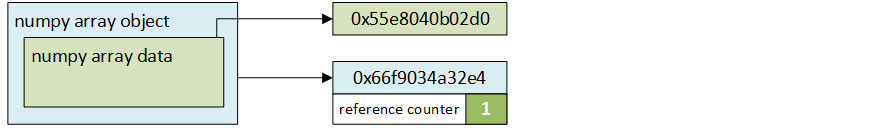
\includegraphics[width=0.99\textwidth]{img/array_creation_deletion_a}
        \caption{The NumPy array is created in Python. Note that the NumPy 
        object and the data it contains are represented by two separate memory addresses.}
        \label{fig:array_creation_deletion_a}
    \end{subfigure}
    \begin{subfigure}{0.9\textwidth}
        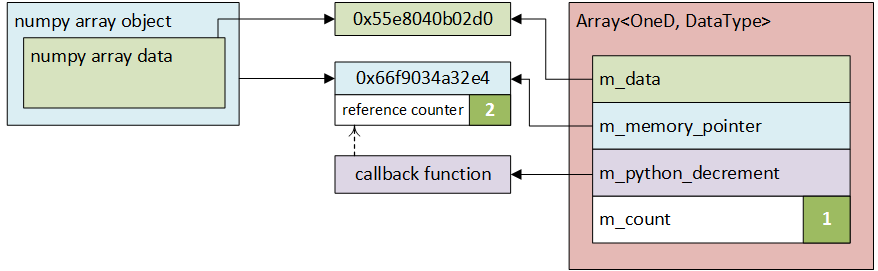
\includegraphics[width=0.99\textwidth]{img/array_creation_deletion_b}
        \caption{The C++ array is created through the converter method: its attributes 
        point to the appropriate memory addresses and the reference counter of the 
        memory address of NumPy array object is incremented.}
        \label{fig:array_creation_deletion_b}
    \end{subfigure}
    \begin{subfigure}{0.9\textwidth}
        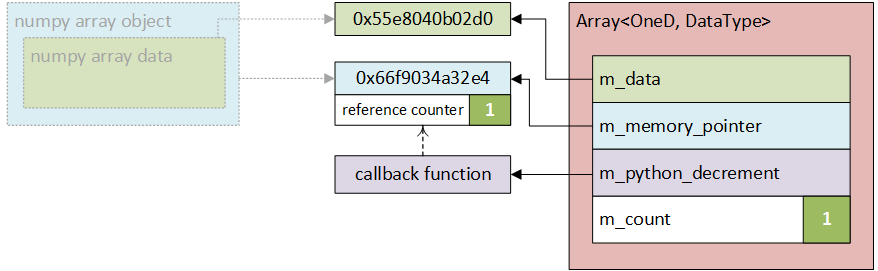
\includegraphics[width=0.99\textwidth]{img/array_creation_deletion_c}
        \caption{If the NumPy object is deleted first, the reference counter is 
        decremented, but the data still exists in memory.}
        \label{fig:array_creation_deletion_c}
    \end{subfigure}
    \begin{subfigure}{0.9\textwidth}
        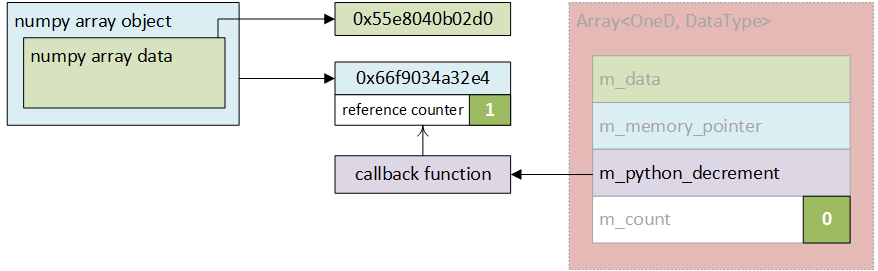
\includegraphics[width=0.99\textwidth]{img/array_creation_deletion_d}
        \caption{If the C++ array is deleted first, the callback function decrements 
        the reference counter of the NumPy object but the data still exists in memory.}
        \label{fig:array_creation_deletion_d}
    \end{subfigure}
    \caption{Diagram showing the process of creation and deletion of arrays. Reference 
    counters shown in green.}
    \label{fig:array_creation_deletion}
\end{figure}

\clearpage

\begin{figure}[h!]
    \centering
    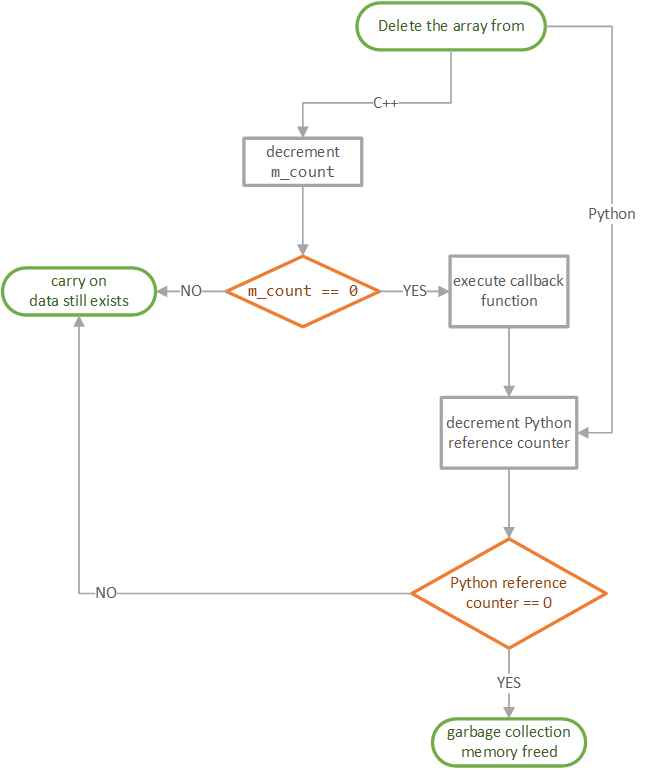
\includegraphics{img/deletion_flowchart}
    \caption{Flowchart describing the procedure for array deletion from either side of 
    the code.}
    \label{fig:array_deletion}
\end{figure}

\clearpage

\begin{lstlisting}[caption={Converter method for converting the Python NumPy arrays into C++ arrays.}, label={lst:python_to_c}, language=C++]
static void construct(
        PyObject *objPtr,
        py::converter::rvalue_from_python_stage1_data* data)
    {
        // Extract data from the PyObject.
        // This has to be a _borrowed_ reference, otherwise at the end of this
        // scope it seems memory gets deallocated
        py::object obj((py::handle<>(py::borrowed(objPtr))));
        np::ndarray array = py::extract<np::ndarray>(obj);
        
        // Get pointer to the memory into which the C++ type will be constructed
        void *storage = (
            (py::converter::rvalue_from_python_storage<Array<OneD, T> >*)data)
            ->storage.bytes;
        data->convertible = storage;
        
        // Grab the address of PyObject for C++ to use.
        void *memory_pointer = objPtr;
        
        // Remedies issues with using const datatypes.
        using nonconst_t = typename std::remove_const<T>::type;
        
        // Construct OneD array from numpy array.        
        new (storage) Array<OneD, T>(array.shape(0), // array size
            (nonconst_t *)array.get_data(), // pointer to the data readable by C++
            memory_pointer, // memory address of the PyObject
            &decrement); // pointer to the callback decrement function
        // Increment the Python reference counter.
        Py_XINCREF(objPtr);
    }
\end{lstlisting}

\subsubsection{Testing}

As the process of converting arrays from Python to C++ required making direct calls to 
C API and relying on custom-written methods, more detailed testing was deemed necessary. 
In order to thoroughly check if the conversion works as expected, three tests were 
conducted to determine whether the array is:

\begin{enumerate}
\item referenced (not copied) between the C++ program and the Python wrapper,
\item accessible to C++ program after being deleted in Python code,
\item accessible in Python script after being deleted from C++ objects.
\end{enumerate}

Python files containing test scripts are currently located in 
\path{library\Demos\Python\tests}. They should be converted into unit tests 
that should be run when Python components are built.

\chapter{FieldConvert in NekPy}

This chapter describes how to emulate the functionality of the
FieldConvert utility in Python using the bindings and wrappers
created for the \verb+FieldUtils+ library.

\section{Idea and motivation}

The primary objective is to allow the user to execute a sequence of
commands from a Python script that implement the functionality of
FieldConvert, thereby giving freedom to customise the order in which
modules are used and which command lines options are passed to them.
One problem with FieldConvert is when the user wishes to perform the same
task on many files; for example converting a number of .chk files to VTK
format. To achieve this using FieldConvert, one must run a command like
the following $n$ times for each individual file.

\begin{lstlisting}[style=BashInputStyle]
FieldConvert -m session.xml field_n.chk field_n.vtu
\end{lstlisting}

These .chk files represent the same fields, only at different moments in
time, and so the mesh described in the session file is the same. For each
file, an instance of \verb+Field+ is initialised and its member variables
populated by the modules \verb+InputFld+, \verb+ProcessCreateExp+, and
\verb+OutputVtk+. This is clearly computationally inefficient. In the Python
implementation, we are able to initialise instances of these classes only
once, and then for each file populate and clear the variables that differ.

\section{User workflow}

The design of the Python interface is to allow the user to instantiate
modules by calling the static \verb+Create+ method of the
\verb+InputModule+,\verb+ProcessModule+, and \verb+OutputModule+,
register configuration options, and run them. For example, consider the command:

\begin{lstlisting}[style=BashInputStyle]
FieldConvert -n 10 -m wss:bnd=0 session.xml field.fld  field_wss.fld
\end{lstlisting}


A Python script performing the same task is given below.

\begin{lstlisting}[style=C++Style, language=Python]
import sys
from NekPy.FieldUtils import *

field = Field(sys.argv, output_points=10)

InputModule.Create("xml",   field, "session.xml").Run()
InputModule.Create("fld",   field, "field.fld").Run()
ProcessModule.Create("wss", field,  bnd="0").Run()
OutputModule.Create("fld" , field, "field_wss.fld").Run()
\end{lstlisting}

The key points are that the FieldConvert command line options, in this
case \inltt{output-points}, are passed to the constructor of \verb+Field+.
The configuration options for a given module are passed to the static
\verb+Create+ method of the \verb+InputModule+,\verb+ProcessModule+, and
\verb+OutputModule+. This creates the corresponding module and the
modules can be run immediately after instantiation. Note that the first
parameter of the \verb+Create+ method has to be the key for a given module,
the second is the field variable and for input and output modules the remaining
arguments may identify the input and output files for a given module.
Optionally we can explicitly specify the file type of an input module
using the "infile" keyword and the "outfile" keyword for output modules.


\begin{lstlisting}[style=C++Style, language=Python]
import sys
from NekPy.FieldUtils import *

field = Field(sys.argv, output_points=10)

InputModule.Create("xml",   field, infile={"xml": "session.xml"}).Run()
InputModule.Create("fld",   field, infile={"fld": "field.fld"}).Run()
ProcessModule.Create("wss", field, bnd="0").Run()
OutputModule.Create("fld" , field, outfile="field_wss.fld").Run()
\end{lstlisting}

Or can also emulate the functionality of FieldConvert when using the
\inltt{nparts} option in the following way. Here \verb+session_xml+ is a
directory containing the mesh partitioned into 2.

\begin{lstlisting}[style=C++Style, language=Python]
import sys
from NekPy.FieldUtils import *

field = Field(sys.argv, nparts=2, forceoutput=True, error=True)

inputxml   = InputModule.Create("xml",   field, "session_xml")
inputfld   = InputModule.Create("fld",   field, "field.fld")
processwss = ProcessModule.Create("wss", field,  bnd="2")
outputfld  = OutputModule.Create("fld",  field, "field_wss.fld")

for part in range(2):
	field.NewPartition(sys.argv, part)
	inputxml.Run()
	inputfld.Run()
	processwss.Run()
	outputfld.Run()

OutputModule.Create("info", field, "field_wss_b0.fld", nparts=2).Run()
\end{lstlisting}

The number of partitions is looped over, with \verb+NewPartition+ called at
the start of each. When using \verb+OutputModule+, the \verb+info+ module
must be used in order to obtain the correct result.

\subsection{Bindings}

\paragraph{Directory structure}


The bindings are stored within a directory named 'Python' in the
\texttt{FieldUtils} directory.

\begin{itemize}
    \item \inlsh{FieldUtils.cpp} is responsible for
		  exporting the \verb+FieldUtils+ Python library.
    \item \inlsh{Field.cpp} contains bindings for the \verb+Field+ struct.
    \item \inlsh{Module.cpp} contains bindings for \verb+Module+,
	      \verb+InputModule+, and \verb+OutputModule+.
\end{itemize}



\bibliographystyle{plain}
\bibliography{developers-guide} 

\printindex

\end{document}
